% * * * * * * * * * * * * * * * * * * * * * * * * * * * * * * * * * * *
% *                             Thesis                                *
% *                 https://github.com/Jacopx/Thesis                  *
% * * * * * * * * * * * * * * * * * * * * * * * * * * * * * * * * * * *

\documentclass[%
    corpo=12pt,
    twoside,
%    stile=classica,
    oldstyle,
    autoretitolo,
    greek,
    evenboxes,
%    tipotesi,
]{toptesi}
%%%%%%%%%%%%%%%%%%%%%%%%%%%%%%%%%%%%%%%%%%%%%%%%%%%%

\usepackage[utf8]{inputenc}
\usepackage[T1]{fontenc}
\usepackage{lmodern}
\usepackage{hyperref}
\usepackage{graphicx}
\usepackage{subfigure}
\usepackage{booktabs}
\usepackage{amsfonts}
\usepackage{amsmath}
\usepackage{amssymb}
\usepackage{bm}
\usepackage{listings}

\hypersetup{%
    pdfpagemode={UseOutlines},
    bookmarksopen,
    pdfstartview={FitH},
    colorlinks,
    linkcolor={blue},
    citecolor={blue},
    urlcolor={blue}
  }

%%%%%%% Definizioni locali

\interlinea{1.5} 


\begin{document}

\ateneo{Politecnico di Torino}

\titolo{Predizione di difettosità nello sviluppo software attraverso machine learning}
\sottotitolo{Apprendimento automatico applicato all'ingegneria del software}

%
%%%%%%% Corso degli studi
\corsodilaurea{Ingegneria Informatica}% per la laurea

\renewcommand*\IDlabel{}
%
\candidato{Jacopo \textsc{Nasi} [255320]}

%%%%%%% Relatori o supervisori
\relatore{prof.~Maurizio \textsc{Morisio}}

%%%%%%% Tutore
\tutoreaziendale{dott.\ Davide \textsc{Piagneri}}

\sedutadilaurea{\textsc{Aprile} 2020}


%%%%%%% Logo della sede
\logosede{polito}


\frontespizio
\summary
Ogni giorno migliaia di commit vengono eseguiti, ognuno di loro contiene molte informazioni: file modificati, modifiche, commenti, registri di test e molto altro. Una strutturata e corretta gestione delle piattaforme di controllo sorgente permette l'estrazione di dati utili analizzabili utilizzando modelli statistici di intelligenza artificiale.\\
Al fine di poter correttamente utilizzare questi dati sono necessari alcuni step preliminari: la prima fase riguarda l'analisi della struttura dati al fine di permettere l'estrazione di tutte le possibili informazioni, successivamente la pre-elaborazione per rimuovere informazioni di inutili e di disturbo, con i dati puliti è possibile procedere con l'estrazione di dati combinati, come la seniority degli sviluppatori, una lista di parole dei componenti modificati, la versione ed altre informazioni di carattere più matematico. L'ultima fase prevede la sostituzione dell'etichetta testuale relativa alla priorità con un valore numerico corrispondente al valor medio della distribuzione della durata di quella etichetta, questo valore prenderà il nome di severity. I dati verranno poi aggregati per settimana.
Una volta generati i dati verranno utilizzati per allenare tre differenti modelli: foresta casuale, aumento di gradiente e rete neurale. L'allenamento sarà gestito in tre differenti modalità: la prima allena e predice utilizzando lo stesso filone di dati, la seconda, cross-version, prevede che il modello venga allenato su dati relativi ad alcune versione del progetto per poi effettuare la predizione sulle successive, la terza, cross-project, allena il modello con dati relativi ad un progetto per poi prevedere l'andamento di uno differente.\\
Tutti le tipologie ottengono dei buoni risultati, il migliore è quello cross-project che riesce ad ottenere una precisione del 90\% fino a quattro settimane e comunque maggiore del 70\% fino a 20 settimane.


\acknowledgements
Un ringraziamento speciale a Smirnuff ed i suoi cavalieri, luce della mia battaglia.

\renewcommand{\baselinestretch}{1.1}\normalsize
\indici
\renewcommand{\baselinestretch}{1.5}\normalsize

\mainmatter

% #######################################
% #            Introduction             #
% #######################################

\chapter{Introduzione}
\label{chap:intro}
\section{Problema Generale}
Lo sviluppo software non si presenta molto differente dallo sviluppo di qualsiasi altro prodotto, dopo una fase iniziale di progettazione lo sviluppo del codice può avere inizio, durante esso emergeranno sistematicamente dei problemi che dovranno essere risolti prima della consegna della versione finale.\\
Ogni progetto software è costituito da diversi commit per giorno, ognugno di essi contiene innumerevoli informazioni le quali possono essere utilizzate per analisi statistiche. La predizione della difettosità può migliorare enormemente il processo di sviluppo, allocando un corretto numero di sviluppatori per risolvere le problematiche e riducendo quindi le tempistiche per la correzione. Anche il machine learning può essere utilizzato per la predizione dei difetti.\\
La predizione è uno strumento sempre più utilizzato a livello industriale, un corretto utilizzo può generare enormi benifici a livello produttivo, permettendo la riduzione di sprechi, l'ottimizzazione delle vendite e tante altri vantaggi. Lo sviluppo di progetti di natura informatica è sempre di più centrale all'interno della nostra società attuale, anche questo processo potrebbe trarre beneficio dai vantaggi della predizione. L'implementazione di tecniche statistiche viene in supporto, vista la natura intellettuale della programmazione, nello generazione di predizioni utili.

\section{Lavori correlati}
L'utilizzo del software ha avuto un vertiginoso aumento negli ultimi anni, il modo dell'informatica si è insediato ormai in tutti i settori della nostra società. L'aumento della richiesta di sviluppo software porta senza dubbio ad una crescente necessità di ottimizzazione nello sviluppo, la riduzione dei costi e l'aumento di efficenza nello sviluppo permette alle aziende di ridurre enormemente i costi. L'ingegneria del software si occupa proprio di studiare queste tecniche. Lungo gli anni sono state sviluppate una moltitudine di tecniche per l'analisi della difettosità nello sviluppo software, le prime, come quelle sviluppate da Akiyama per Fujitsu \cite{Akiyama1971AnEO} si basavano su calcoli matematici basati sulle linee di codice (LoC) per supporre il numero di errori, altre tecniche sfruttavano valori direttamente correlati con il linguaggio, come lo studio di Halstead \cite{halstead1977elements}. In generale tutti questi studi cercavano la difettosità all'interno del codice vero e prorio. I primi studi basati sul livello funzionale,sfruttando tecniche statiche di regressione lineare, fuorono condotti da Graves \cite{graves_se}, Rathore e Kumar \cite{santosh_se} hanno sperimentato l'ultilizzo degli alberi decisionali, più recentemente hanno anche trattato altri algortimi d'insieme \cite{rathore}. In maniera molto simile a come verrà trattato in questo elaborato, Chen \cite{Chen} ha valutato sei differenti modelli tra cui l'albero decisionale, applicando tecniche cross-version e cross-project. Anche \cite{super_unsuper} hanno applicato le medisime tecniche\\
Al momento della stesura di questo elaborato non esiste ulteriore letteratura riguardo al database utilizzato. Alcuni dei modelli che verranno utilizzati sono stati trattati, come citato, non vi è alcuna letteratura sull'applicazione di reti neurali a questa tipologia di problematica.

\section{Strumenti utilizzati}
Lo sviluppo di questo progetto a richiesto l'utilizzo di diversi strumenti, di seguito una lista degli stessi:

\paragraph{\href{https://www.python.org/}{Python}} Il linguaggio di programmazione principale, utilizzato per la gestione dei dati, l'estrazione di informazioni, l'applicazione di algoritmi matematici e l'interazione con altri software. Nello specificio la versione utilizzata è stata la v3.7.0

\paragraph{\href{https://pandas.pydata.org/}{Pandas}} Libreria open source ad alte prestazioni, con semplici strutture e strumenti adatti all'analisi dati attraverso Python.

\paragraph{\href{https://numpy.org/}{NumPy}} Libreria per il calcolo scientifico attraverso Python.

\paragraph{\href{https://matplotlib.org/}{Matplotlib}} Libreria per il disegno di grafici 2D in Python.

\paragraph{\href{https://seaborn.pydata.org/}{Seaborn}} Libreria avanzata per il disegno 2D in Python.

\paragraph{\href{https://www.tensorflow.org/}{Tensorflow}} Piattaforma per machine learning.

\paragraph{\href{https://keras.io/}{Keras}} API di alto livello per reti neurali.

\paragraph{\href{https://scikit-learn.org/stable/}{SciKit-Learn}} Strumenti e librerie per machine learning.

\paragraph{\href{https://gitlab.com}{GitLab}} Piattaforma di sourcing basata su Git. Utilizzata per il codice sorgente del progetto.
% \url{https://gitlab.com/EiS-Projects/analytics/temp/thesisProjectJN}.

\paragraph{\href{https://github.com}{GitHub}} Piattaforma di sourcing basata su Git. Utilizzata per il calendario e elaborato testuale:
\begin{itemize}
  \item Tesi: \url{https://github.com/Jacopx/Thesis}
  \item Calendario: \url{https://github.com/Jacopx/ThesisCalendar}
\end{itemize}

\paragraph{\href{https://www.jetbrains.com/}{JetBrains IDEs}} IDE per lo sviluppo di diversi linguaggi di programmazione, gratuita per gli studenti:
\begin{itemize}
  \item PyCharm: \url{https://www.jetbrains.com/pycharm/}
  \item DataGrip: \url{https://www.jetbrains.com/datagrip/}
\end{itemize}


% #######################################
% #              Datasets               #
% #######################################

\chapter{Dati}
\label{chap:dataset}
Le seguenti sezioni analizzeranno le basi di dati utilizzate in questo progetto.
\section{SEOSS33}
SEOSS33\cite{SEOSS33} è una \href{https://doi.org/10.7910/DVN/PDDZ4Q}{base dati} collezionante errori, issue e tante altre informazioni a proposito di 33 progetti open source. I dati sono stati tutti collezionati estraendo le informazioni dalle piattaforme di controllo del codice sorgente, Version Control System (VCS), come GitHub e dalle piattaforme per la gestione dello sviluppo, Issue Tracking System (ITS), come Jira di Atlassian.\\
Ad oggi nessun altro progetto di ricerca, su questi dati, è stato effettuato.\\
Ogni progetto prevede una propria linea durante la fase di sviluppo, tutte le metodologie e linee guida sono alla base degli studi di ingegneria del software. Tuttavia è possibile unificare ed accorpare secondo una categorizzazione standar molte delle differenze specifiche. Lo svilluppo della base dati SEOSS33 mira proprio alla creazione di un serie di dati generalizzati e fruibili attraverso medesime procedure senza la necessità di adattarsi alle specifiche caratteristiche di ogni singolo progetto.\\
Il mondo open source presenta una quantità pressochè infinita di differenti software, parte del progetto in questione è stata dedicata alla selezione dei software da analizzare per l'inserimento nella base dati condivisa, per questo motivo sono state definite alcune carattestiche che accomunassero i vari progetti in modo da costituire una base: discretamente omogenea a livello di dimensionalità, ma con differenze struttuali utili per successive analisi come quella relativa a questo progetto. Il requisito principiale riguardava il linguaggio di programmazione, considerare progetti sviluppati per la maggior parte in un singolo linguaggio di programmazione permette di ridurre la variabilità interna ad ogni singolo progetto. Vista la natura di analisi attraverso il machine learning, un'altra importante carattestica riguardava il numero di issue, il quale doveva essere sufficientemente elevato. I progetti, oltre a dover essere attualmente in sviluppo, dovevano presentare un età di almeno 3 anni. La definizione di tutti questi parametri a permesso di generare una base dati contenente 33 progetti simili come struttura ma con caratteristiche differenti.\\
Lo sviluppo del presente progetto di tesi si è concentrato solamente su cinque di questi schemi, sono stati scelti i progetti più grossi e quelli in sviluppo dal maggior tempo, nello specificio i selezionati sono riportati in tabella \ref{tab:seoss33_selected}:
\begin{center}
  \captionof{table}{Distribuzione dati} \label{tab:seoss33_selected}
  \begin{tabular}{ |c|c|c| }
     \hline
     \textbf{Progetto} & \textbf{Mesi} & \textbf{Issue} \\
     \hline
     \hline
     Hadoop & 150 & $39086$ \\
     Hbase & 131 & $19247$ \\
     Maven & 183 & $18025$ \\
     Cassandra & 106 & $13965$ \\
     Hive & 113 & $18025$ \\
     \hline
  \end{tabular}
\end{center}

Al fine di generalizzare le specifiche differenze, le varie issue: \textit{New Feature}, \textit{Bug Report}, ecc... Sono state mappate su cinque categorie:
\begin{itemize}
  \item Bug: Un problema che previene il funzionamento del prodotto
  \item Feature: Una nuova funzionalità del prodotto
  \item Improvement: Un miglioramento di una funzionalità già esistente
  \item Task: Un compito necessario
  \item Other: Vario
\end{itemize}

La figure \ref{fig:prior} visualizza la distribuzione, rispetto le varie categorie, del numero di issue per ogni progetto.
\begin{figure}[!ht]
  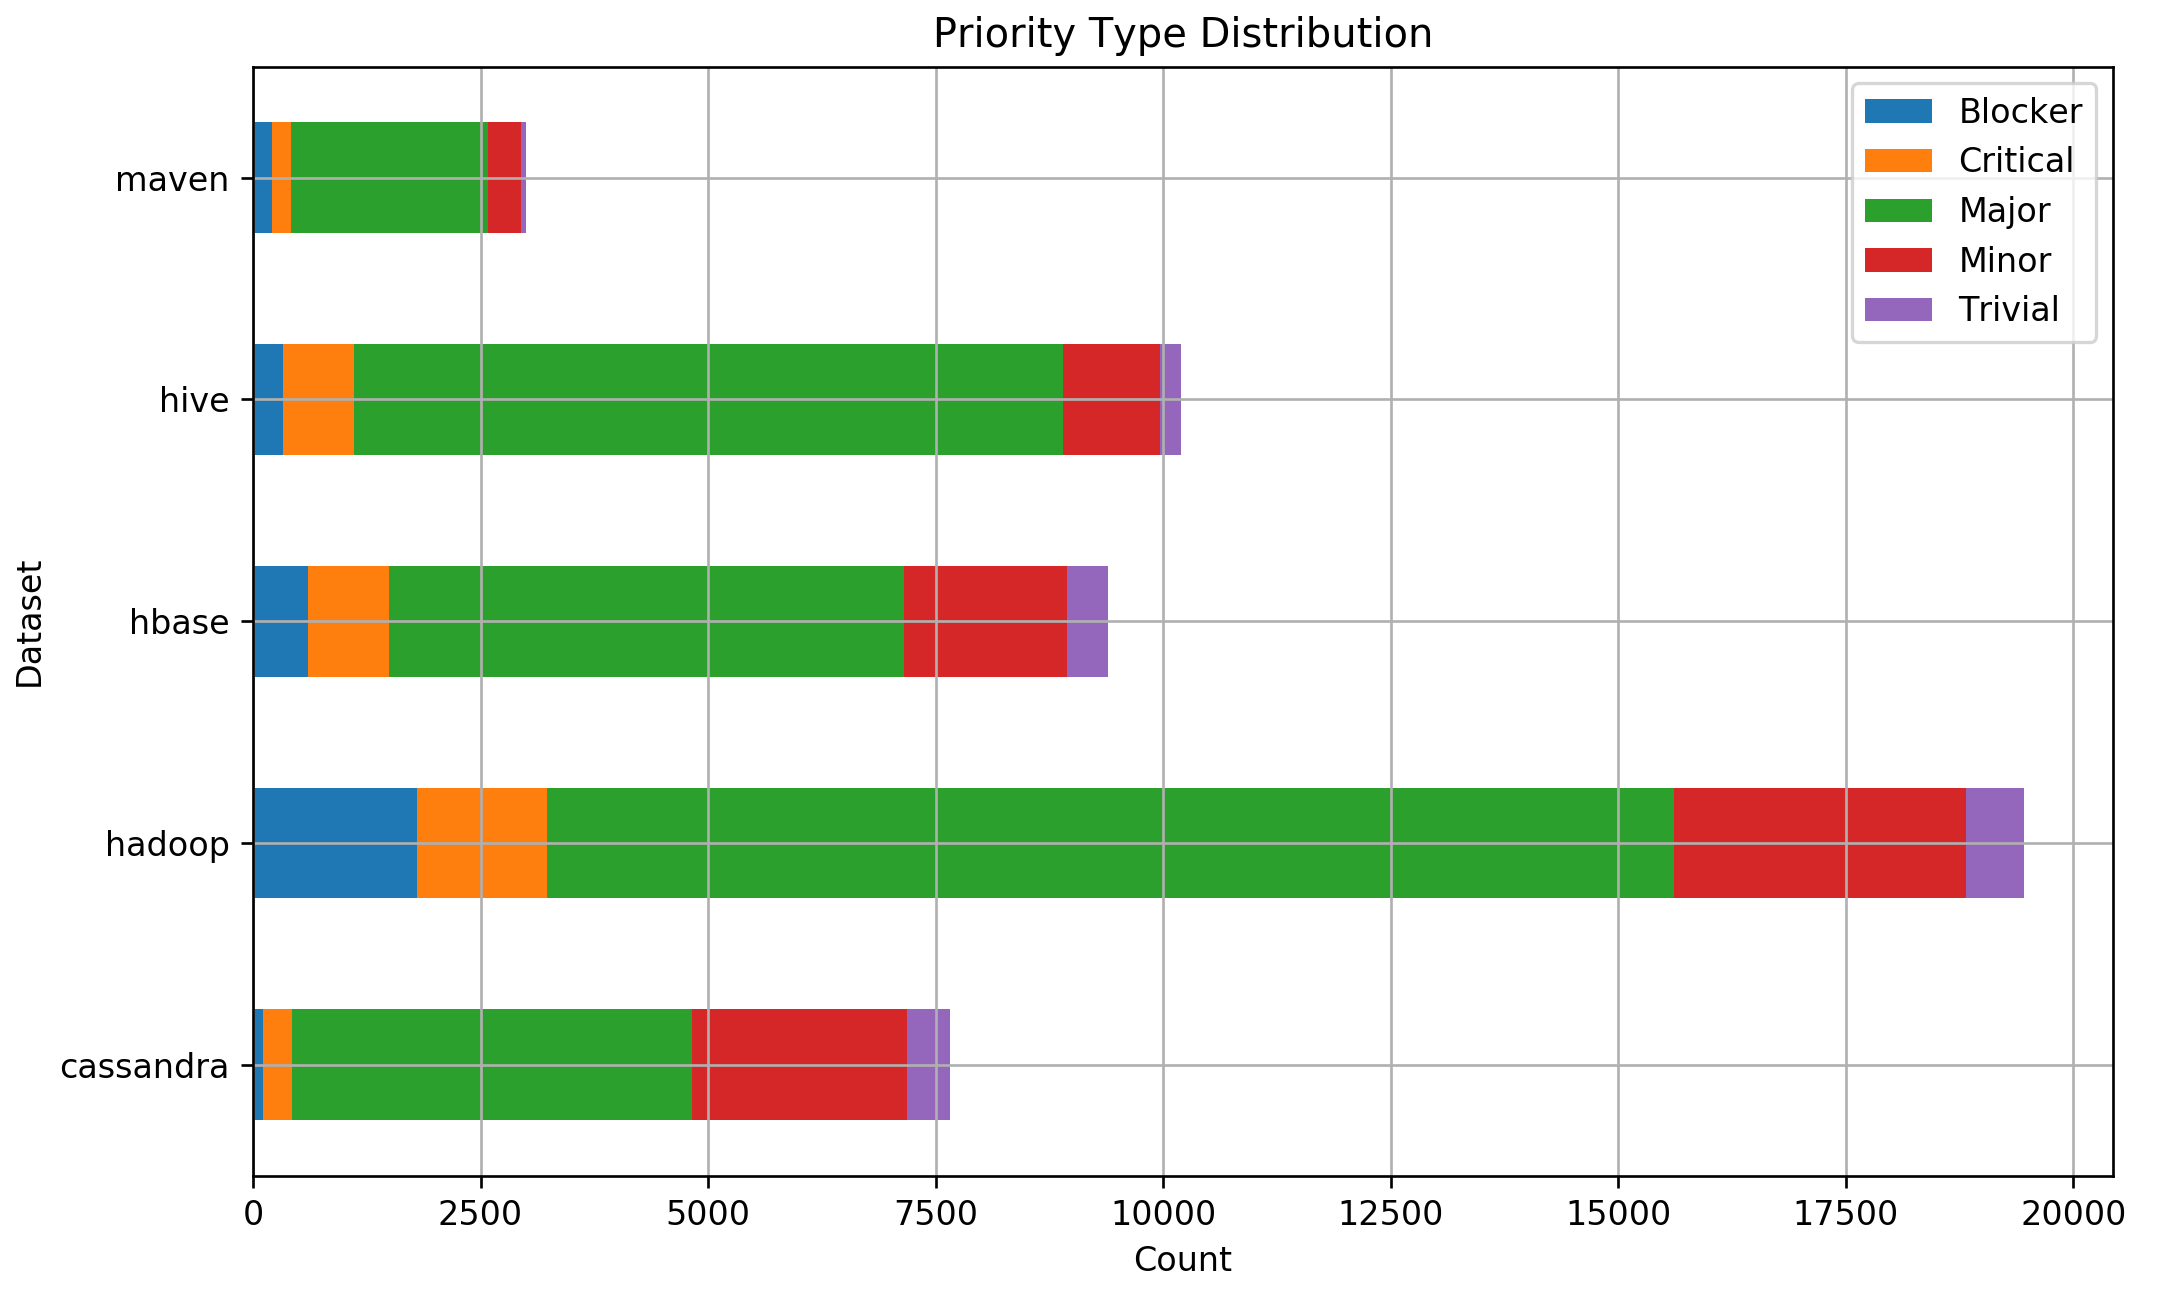
\includegraphics[width=\linewidth]{figure/prior.png}
  \caption{Distribuzione issue per progetto}
  \label{fig:prior}
\end{figure}
Per poter estrarre ed utilizzare al meglio i dati è necessario conoscere al meglio la struttura contenitore.
I dati relativi ad ogni software sono salvati in un file SQLITE, un database SQL offline che permette l'accesso sfruttando le potenzialità delle query, senza la necessità di un server vero e proprio. La figura \ref{fig:seoss33_db} riporta lo schema integrale della struttura.\\
Tutto il modello si basa sulla sua entità centrale, la issue, ovvero l'attività di segnalazione che è stata creata da uno sviluppatore per gestire una problematica. Ognugna di queste issue è caratterizzata dal proprio \textit{issue\_id} il quale ne rappresenta la chiave primaria ed univoca, normalmente è strutturata con il nome del progetto seguito da un numero progressivo. La tabella relativa alle issue contiene ulteriori informazioni direttamente correlate, la tipologia, la priorità, le informazioni temporali di apertura, aggiornamento e chiusura della stessa, un breve riassunto della problematica, lo stato e le informazioni relative allo sviluppatore che l'ha aperta. Direttamentamente collegate, tramite la chiave primaria, vi sono le tabelle contenenti i commenti \textit{issue\_comment}, la versione \textit{issue\_fix\_version}, il componente modificato \textit{issue\_component} ed la tabella \textit{change\_set\_link} la quale collega i vari commit alle issue. Durante l'estrazione delle varie informazioni sono state utilizzate tute le tabelle ad esclusione di \textit{issue\_link} la quale viene utilizzare per correlare le differenti issue tra di loro.

\begin{figure}[!ht]
  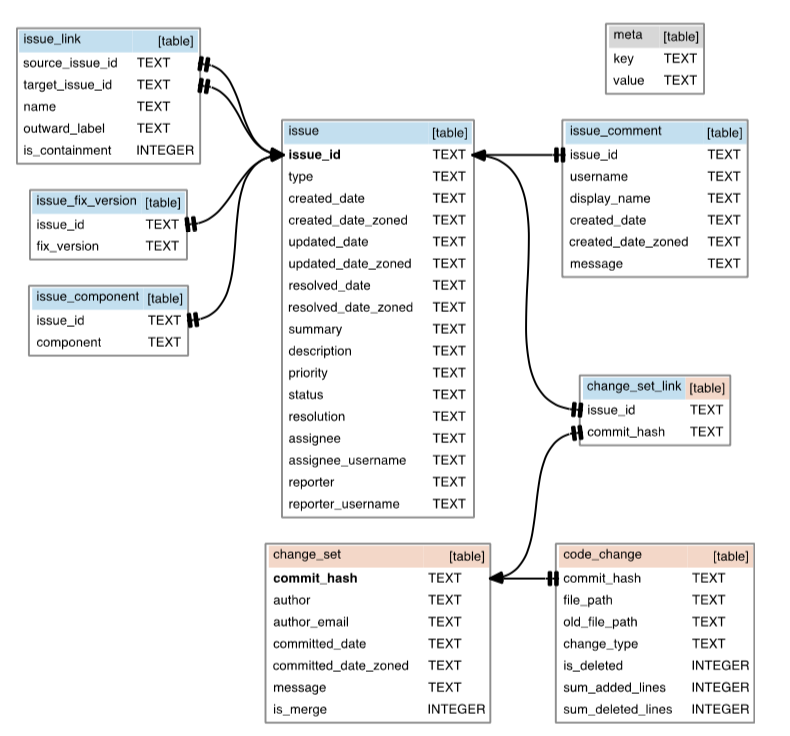
\includegraphics[width=\linewidth]{figure/seoss33_db_schema.png}
  \caption{Struttura dati di SEOSS33}
  \label{fig:seoss33_db}
\end{figure}

% NOTE: Possibile aggiunger parte relativa all'interfacciamento con questo DB. Informazioni di distribuzione temporale.

% #######################################
% #          Machine Learning           #
% #######################################

\chapter{Apprendimento Automatico}
\label{chap:ml}
\section{Introduzione}
L'apprendimento automatico, meglio conosciuto come Machine Learning (ML), è una branca dell'intelligenza artificiale basata sullo studio di algoritmi e modelli statistici utilizzabili dai calcolatori per svolgere determinati compiti senza essere esplicitamente istruiti per farlo. Questa settore è ormai diventato di dominio pubblico, solo negli ultimi decenni l'ultilizzo di queste tecniche è cresciuto enormemente nonostante la maggior parte di esse furono teorizzate già molti anni prima. La motivazione principale di questo ritardo è da ricercare nella natura stesso di queste strategie, la capacità computazione diventa rilevante e fondamentale all'applicazione degli stessi, grazie alla crescita di essa è ora possibile sfruttare questi algorirmi anche nei computer di casa.\\
Tutti gli algoritmi possono essere catalogati in una delle seguenti categorie:
\begin{itemize}
  \item Knowledge-based: Acquisizione e modellazione di leggi conosciute (dalle regole ai fatti)
  \item Learning: Estrazione della conoscenza e delle regole attraverso esempi ed esperienza (dai fatti alle regole)
\end{itemize}
Tutti gli algoritmi in ambito ML fanno parte della seconda categoria. A loro volta questi algoritmi possono essere divisi in tre principali sotto-categorie: apprendimento supervisionato, apprendimento non supervisionato e apprendimento per rinforzo. Nel primo vengono forniti modelli di dati in ingresso e i dati desiderati in uscita e lo scopo è quello di definire una regola che associ i due parametri. Nel modello non superivisionato il modello ha il compito di trovare una struttura ai dati in ingresso, senza che essi siano precedentemente etichettati in alcun modo. L'ultimo invece viene allenato per un compito, senza che gli venga insegnato come fare ma solamente conoscendo il risultato finale delle proprie azioni.\\
Esisto una varietà enorme di modelli di questa tipologia, i successivi paragrafi tratteranno quelli utilizzati in questo progetto.

\paragraph{Apprendimento Supervisionato}
è una tecnica che prevede di processamento dei dati in ingresso con associati i valori desiderati in uscita, lo scopo del modello è quindi quello di sviluppare una correzione matematica tra tutte le informazioni che riceve in ingresso ed i valori desiderati in uscita. Un volta terminata la fase di allenamento il modello potrà essere utilizzato per prevedere il valore di uscita dati i valori in ingresso. Questa metodologia può essere applicata nella risoluzione di problemi di due differenti categorie, quelli della classificazione e quelli della regressione lineare. Lo scopo del primo è quello di assegnare una etichetta ai dati per classificarli in diverse categorie, per esempio le transazioni sane o fraudolente di una banca. L'assegnazione può essere binaria, quindi solo due etichette, o multi-etichetta. La regressione invece ha l'obbiettivo di predirre un valore continuo di uscita, cercare di sviluppare una relazione matematica tra tute le variabili in ingresso, cercando di prevedere, con il miglior livello di approssimazione il valore finale. Nel nostro progetto verranno solo impiegati questi ultimi, la classificazione non verrà ulteriormente trattata.

\section{Apprendimento d'insieme}
L'apprendimento d'insieme raggruppa unsa serie di tecniche sviluppate al fine di migliorare i risultati dei singoli prendittori. Invece che utilizzare un singolo modello, nella fase di apprendimento, vengono simultaneamente allenate diverse copie dello stesso modelo con parametri differenti, ciò porterà ad una differenziazione delle risultato di previsione. L'aggregazione, attraverso techinche come bagging, boosting o stacking, permetterà di produrre un risultato più accurato e meno dipendente dalla rumorosità dei dati.

\paragraph{Foresta casuale}
conosciuta anche come Random Forest (RF) è un algoritmo di apprendimento supervisionato, basato sulle metodologie d'insieme, per la classificazione e la regressione. È costituito combinando la predizione di diversi alberi, ognungno allenato separatamente, tramite media \cite{RF_theory}. In figura \ref{fig:rf} una visualizzazione del modello.

\begin{figure}[!ht]
  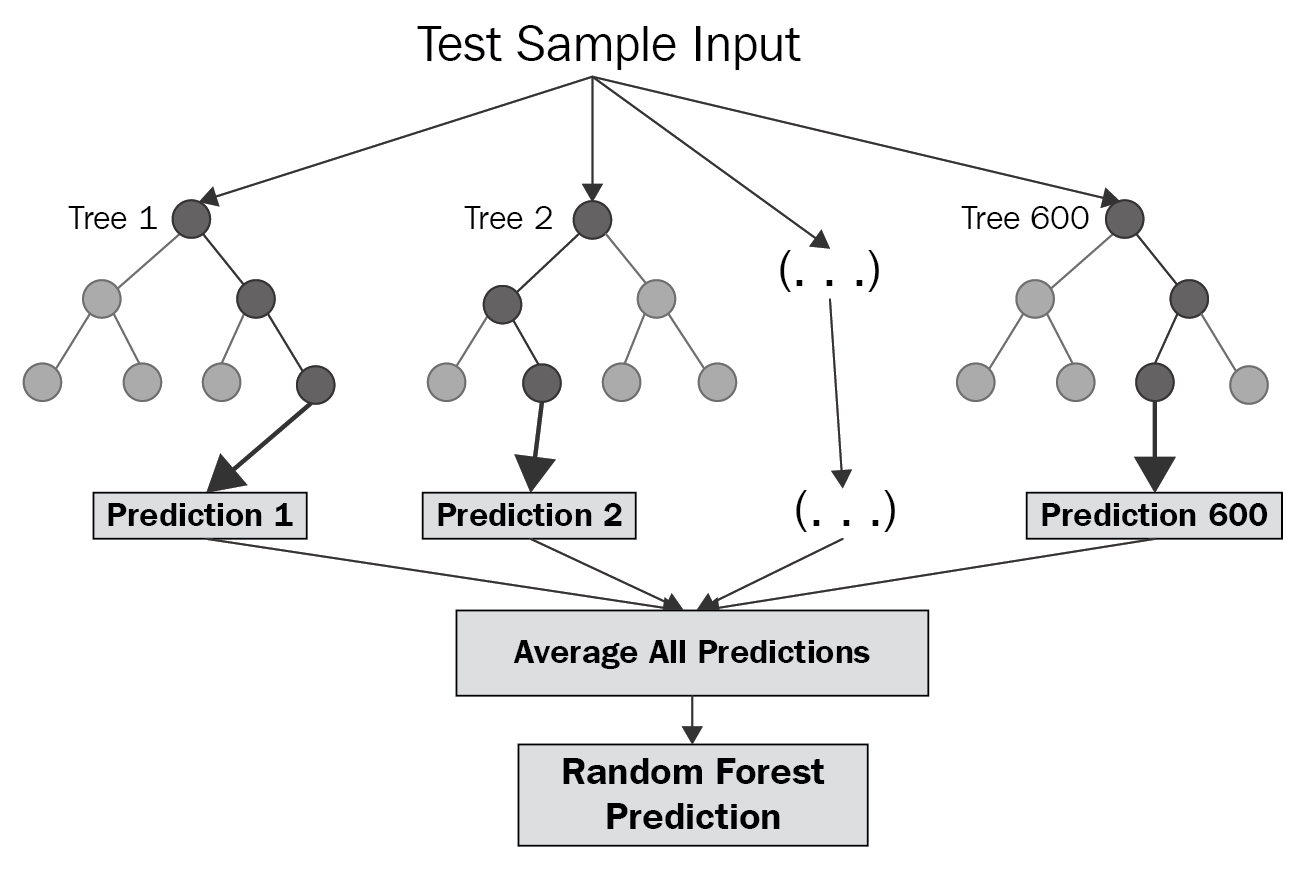
\includegraphics[width=\linewidth]{figure/rf.png}
  \caption{Schema semplificato di foresta casuale \cite{rf}}
  \label{fig:rf}
\end{figure}

La definzione di una foresta richiede tre parametri principali: (1) la metodologia per la divisione in foglie, (2) il tipo di predittore da usare in ciascuna foglia e (3) il metodo per garantire la randomicità.
La divisione in foglia richiede la selezione della forma e metodologia per la valutazione di ogni candidato. Una tipica scelta è quella chiamata axis-aligned, dove i dati vengono diretti nei vari sotto alberi in base al passaggio o meno di un valore soglia, il quale viene scelto casualmente o dalla funzione di ottimizzazione della foglia. Al fine di dividere una foglia vengono generati diversi candidati e viene definito un criterio per scegliere tra essi. Un primo approccio potrebbe essere quello della selezione causuale uniforme, altrimenti la scelta può essere guidata da una funzione di purezza, cercandone la massimizzazione.\\
Possono essere utilizzate diverse techniche per generare casualità nella foresta, attraverso la definizione di soglie senza l'utilizzo di funzioni oppure effettuando con l'allenamento di ogni albero su una selezione di dati ristretta in modo da diversificare direttamente il risultato a livello di insieme.\\
La fase di training viene gestita indipendentemente da ogni alberto attraverso punteggi di struttura e stima, i primi permettono la variazione della forma dello stesso, mentre i secondi guidano le funzioni di ottimizzazione delle singole foglie.\\
Un volta effettuato l'allenamento della rete è possibile utilizzare il modello per la predizione dei valori. Nella fase di stima, ogni singolo albero, generera indipendemente un proprio valore, la scelta finale avverrà calcolando la media aritmetica di tutti questi valori generati, il contributo è equamente ripartito tra tutti.\\
La nostra implementazione sfrutta le API per la Random Forest di SciKit-Learn v0.21:
\begin{lstlisting}[language=python, frame=single]
  from sklearn.ensemble import RandomForestRegressor
\end{lstlisting}
Gli specifici parametri utilizzati verranno illustrati durante il capitolo \ref{chap:forecasting} sulla predizione.

\paragraph{Macchine ad aumento di gradiente}
conosciute anche come Gradient Boosting Machines (GBM), sono una famiglia di potenti modelli statistici di apprendimento automatico in grado di ottenere ottimi risultati in una grande varietà di applicazioni. Una delle loro principali caratteristiche è la possibilità di personalizzare il modello in base alle caratteristiche dell'applicazione \cite{gbm}. Tecniche come la foresta casuale, appena trattata, sono basate sulla semplice media dei risultati prodotti da ogni singolo componente. La famiglia dei metodi di aumento è basata su una differente strategia di unione dei pezzi per la formazione della modello finale. Il boosting aggiunge, sequenziamente, nuovi parti all'insieme; durante la fase di allenamento vengono via via sviluppati nuovi piccoli modelli da aggiungere al fine di migliorare l'accuratezza nella previsione. Idealmente vengono costruiti nuovi modelli di base, come per esempio l'albero decisionale, per poter massimizzare la correlazione con il gradiente negativo della funzione di perdita (\textit{loss}).\\
Vista l'alta flessibilità del modello, l'adattamento dello stesso a differenti ambienti non risulta difficoltoso, molte differenti sperimentazioni possono essere fatte.\\
Nel nostro progetto si è deciso di implementare il modello di Gradient Boosting Decision Tree (GBDT) sempre utilizzando la libreria SciKit-Learn v0.21:
\begin{lstlisting}[language=Python, frame=single]
  from sklearn.ensemble import GradientBoostingRegressor
\end{lstlisting}


\section{Reti Neurali}
Le reti neurali, in inglese Neural Networks (NN), sono modelli di apprendimento automatico con diretta ispirazione al cervello umano e come esso procede alla fase di apprensione di un concetto, la rete è costituita dala basilare unità di calcolo, il neurone (neuron), collegata ad altri neuroni attraverso le sinapsi (synapses). La conoscenza è data alla rete, enlla fare di allenamento, attraverso esempi, la forza delle connessione inter neurali è la base per acquisire e mantenere al conoscenza.\\
La fase di apprendimento può essere sia supervisionata che non supervisionata. La modalità supervisionata viene utilizzata per il riconoscimento di schemi (pattern recognition) e regressione e viene effettuata sempre con i dati di input ed i desiderati dati di output. Invece, la modalità non supervisionata, è maggiormente utilizzata per sviluppare modelli adatti al raggruppamento (clustering) e l'allenamento viene effettuato senza il valore desiderato. Il nostro progetto farò uso di reti neurali per la regressione.\\
Questa tipologia di reti può essere di tre tipologie:
\begin{itemize}
  \item Singolo livello flusso in avanti
  \item Multi livello flusso in avanti
  \item Ricorsiva
\end{itemize}
L'architettura standard è composta di tre diversi livelli, figura \ref{fig:mlff}, lo strato di ingresso, le unità nascoste e il livello di uscita; tutti questi livelli sono correlati tra loro tramite le connessioni sviluppate durante la fase di apprendimento.
\begin{figure}[!ht]
  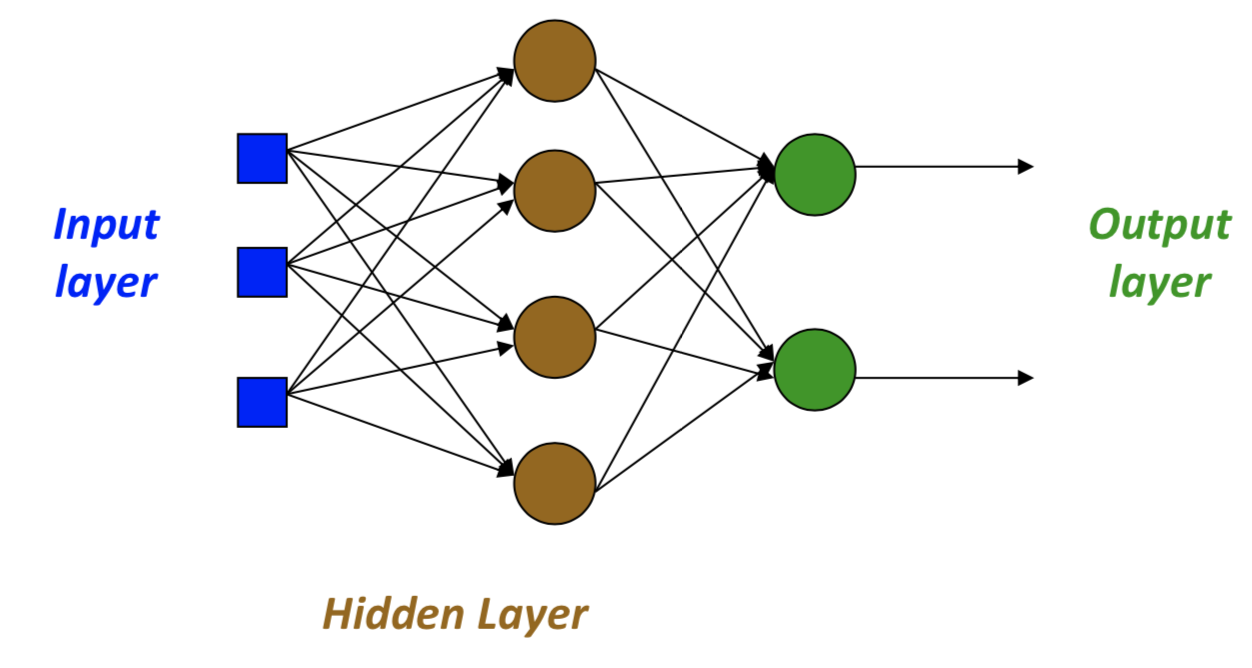
\includegraphics[width=\linewidth]{figure/feed_foward.png}
  \caption{Rete a flusso avanti multi livello}
  \label{fig:mlff}
\end{figure}
Il neurone è l'unità basilare per il processamento all'interno della rete, si occupa di riceve i dati in ingresso, gestirli e poi passarli ai successivi livelli. Ogni ingresso combina i dati con il proprio stato interno e la funzione di attivazione per poi procedere a passare il valore come ingresso del livello successivo. L'importanta che ognugno di questi valori in ingresso avrà sarà determinata dal peso assegnato alla connessione durante la fase di allenamento della rete stessa. Ogni nodo ha la possibilità di ricevere più in un ingresso, per questo motivo, tutti i valori verranno aggregati in modo da consegnare un solo valore come ingresso del successivo strato, la formula per il calcolo della somma è:
\begin{center}
  \begin{equation}
    u = \sum^{m}_{j=1} w_{j}x_{j}
  \end{equation}
\end{center}
Il valore calcolato viene scalato tramite una functione di attivazione $\varphi$ al fine di limitarne l'ampiezza:
\begin{center}
  \begin{equation}
    y = \varphi(u + b)
  \end{equation}
\end{center}
La precedente funzione riporta il parametro $b$ il quale rappresenta il bias, un parametro esterno del neurone. $y$ rappresenta invece il valore di uscita dopo la computazione, il quale rappresenta il valore di ingresso del successivo livello gerarchico. Un esempio della struttura in questione si può trovare in figura \ref{fig:neuron}.
\begin{figure}[!ht]
  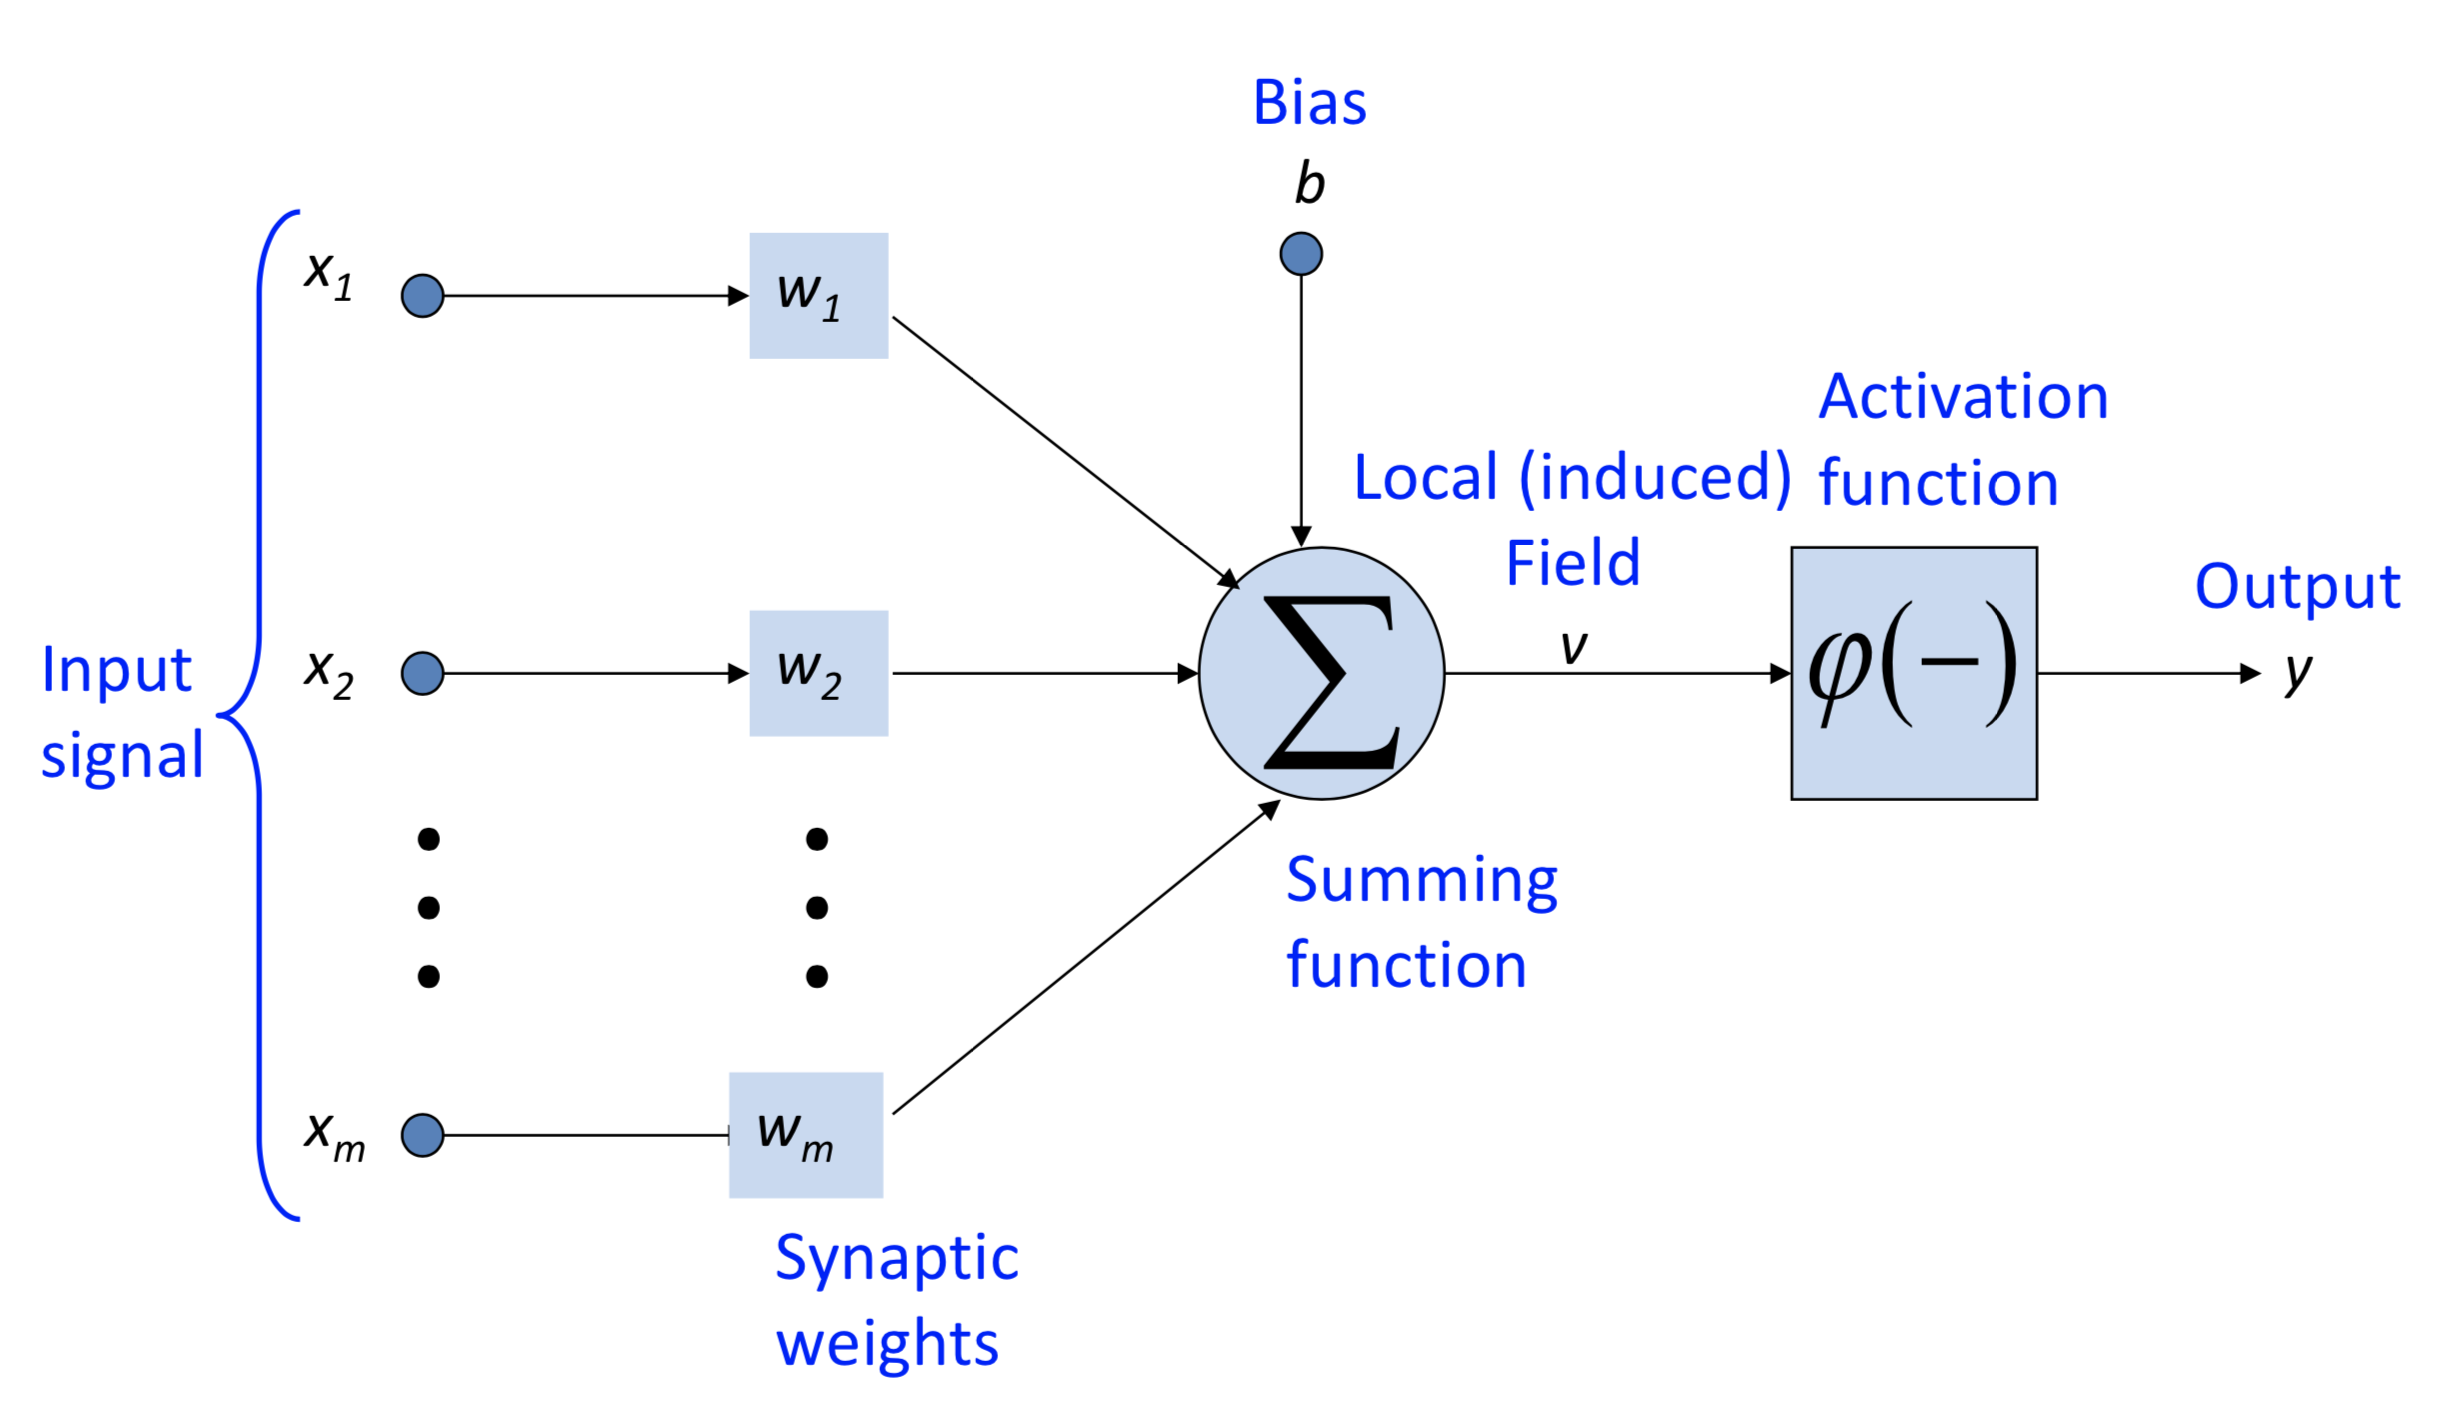
\includegraphics[width=\linewidth]{figure/neuron.png}
  \caption{Visualizzazione di neurone}
  \label{fig:neuron}
\end{figure}

Diverse funzioni di attivazione possono essere applicate al neurone, il loro compito è quello di emulare la tipica risposta biologica del sistema nervoso umano e le sue differenti metodologie di attivazione. Nel corso degli anni sono state definite numerose differenti funzioni, più o meno adatte a differenti contesti, con proprie peculiarità, problematiche e carattestiche. Possono essere classificate in due categorie, lineari e non lineari, le più comuni sono: lineare, gradino, relu e sigmoide.

\paragraph{Gradino} è una delle più comuni funzioni di attivazione, binaria, lineare e basata su soglia, in figura \ref{fig:step} la sua definizione. Quando il valore in ingresso è sopra o sotto la soglia definita, il neurone viene attivano e passa il valore in ingresso al successivo livello. La principale problematica correlata a questa funzione è la sua impossibilità di gestire valori multipli in uscita.

\paragraph{Lineare} è una funzione di attivazione lineare della forma:
\begin{center}
  \begin{equation}
    f(x) = x
  \end{equation}
\end{center}
La funzione, dato il valore in ingresso e moltiplicandolo per il peso del neurone, calcola il valore di uscita. Rispetto alla funzione gradito possono essere generati output multi valore, presenta comunque due problematiche: non sarà possibile utilizzare la retropropagazione (trattata successivamente) per allenare la rete, vista la funzione derivata costante; l'altro problema riguarda il collasso di tutto i diversi livelli in uno solo, vista la sua natura lineare, il valore di uscita finale sarà in ogni caso la combinazione lineare tutti i livelli precedenti. La figura \ref{fig:linear} visualizza la curva in questione.

\begin{figure}
  \centering
  \begin{minipage}{.5\textwidth}
    \centering
    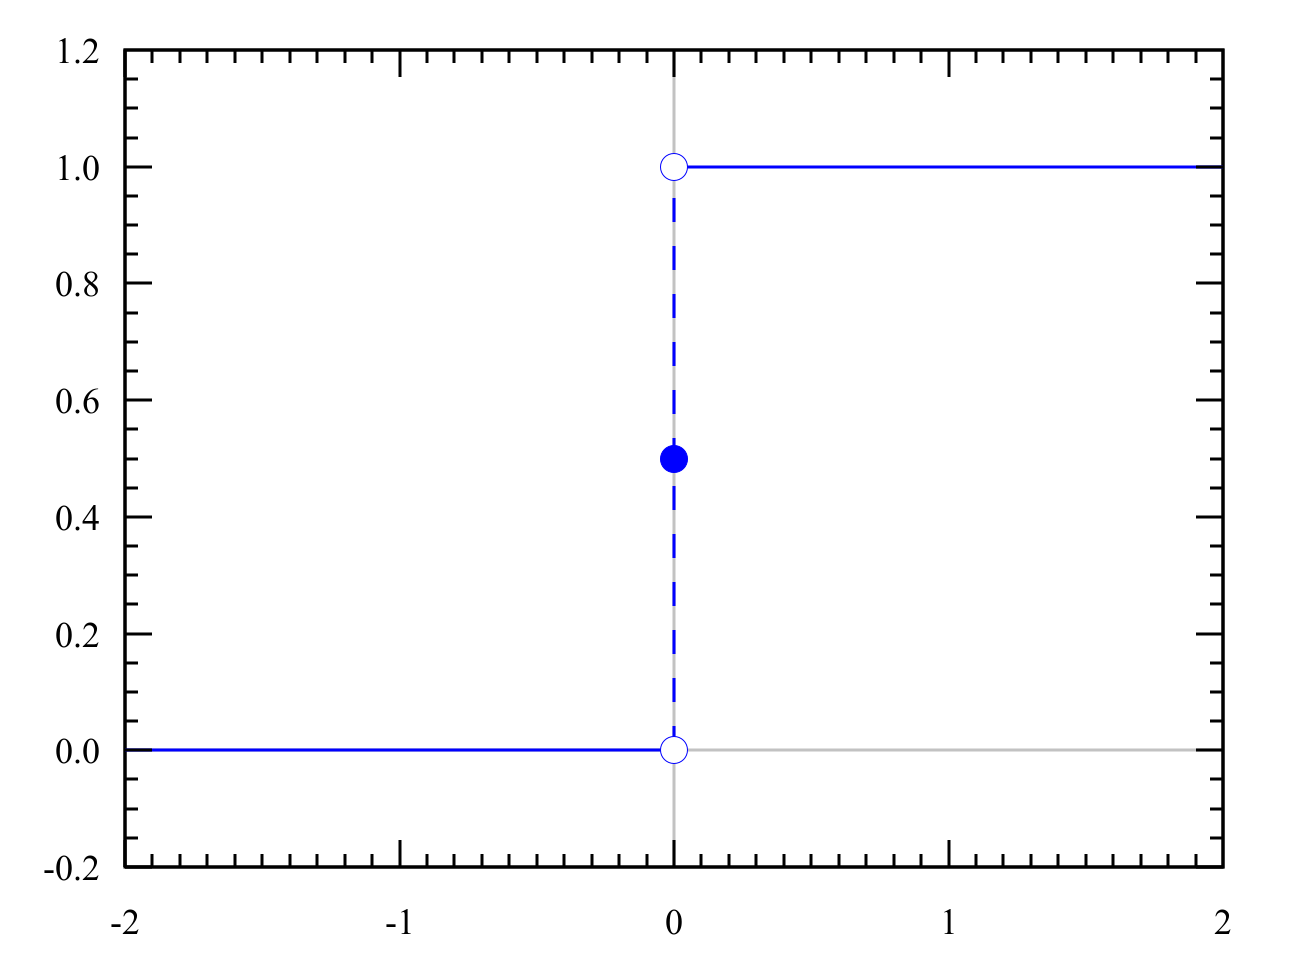
\includegraphics[width=0.85\linewidth]{figure/step.png}
    \caption{Funzione a gradino}
    \label{fig:step}
  \end{minipage}%
  \begin{minipage}{.5\textwidth}
    \centering
    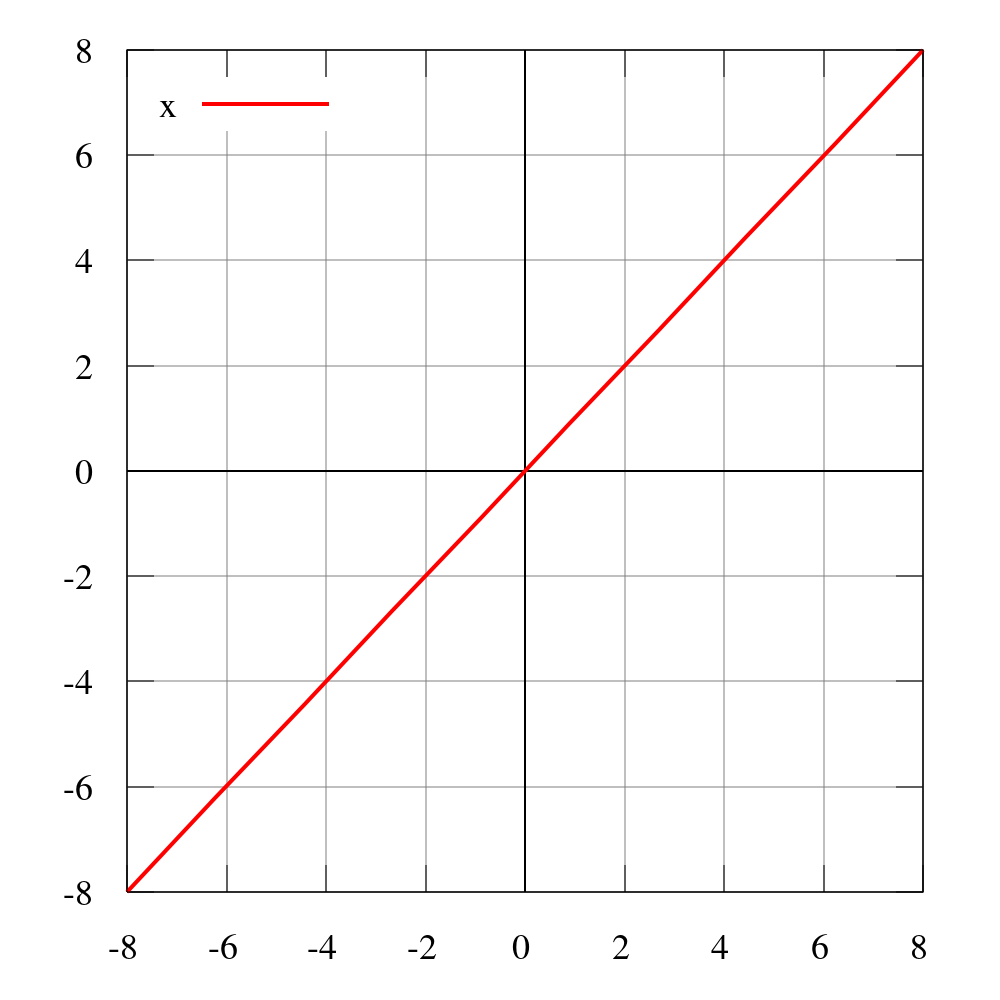
\includegraphics[width=0.75\linewidth]{figure/linear.png}
    \caption{Funzione lineare}
    \label{fig:linear}
  \end{minipage}
\end{figure}

\paragraph{Sigmoide} è la prima funzione di attivazione non lineare trattata, nello specifico è caratterizzata dalla seguente equazione:
\begin{center}
  \begin{equation}
    f(x) = \frac{1}{1+e^{x}}
  \end{equation}
\end{center}
La peculiare caratteristica di non linearità permette un più morbido gradiente in modo da prevenire valori vuori scala, normalizzando il valore tra $[0, +1]$ si ottengono anche benifici a livello di pulizia dei dati in ingresso utilizzati successivamente per le previsioni. La funzione non si presenta esente da problematiche, la principale riguarda la vanificazione del gradiente, se da un lato permette di smorzare i valori fuori scala, si tramuta in collo di bottiglia in altri casi, in caso di valori in ingresso molto elevati o molto bassi non vi sarà differenziazione nel valore di uscita. Inoltre l'applicazione del calcolo stesso è decisamente più impegnativa a livello computazione. La figure \ref{fig:sigmoid} descrive la curva in questione.

\paragraph{ReLU} il quale acronimo sta per Rectified Linear Unit, unità lineare rettificata, è definita nella seguente maniera:
\begin{center}
  \begin{equation}
    f(x)= max(0, x)
  \end{equation}
\end{center}
Nonostante assomigli molto alla funzione di attivazione lineare, presenta una funzione derivate che permette la retropropagazione e si presenta molto efficiente a livello computazione. Le problematiche si presentano in caso di valori in ingresso prossimi allo zero o addirittura negativi, il gradiente della funzione diventa nullo e la rete non potra effettuare la retropropagazione e conseguentemente non potrà portare avanti il processo di apprendimento.

\begin{figure}
  \centering
  \begin{minipage}{.5\textwidth}
    \centering
    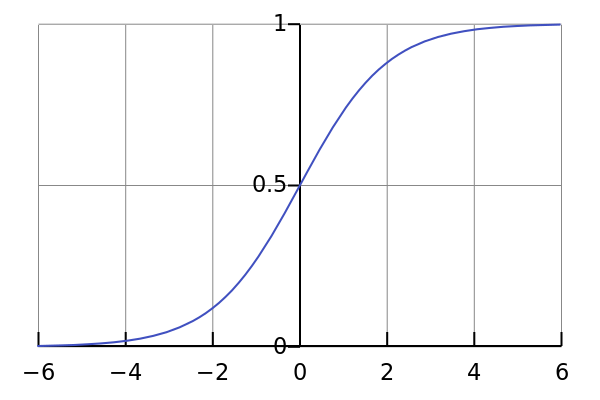
\includegraphics[width=0.8\linewidth]{figure/sigmoid.png}
    \caption{Sigmoide}
    \label{fig:sigmoid}
  \end{minipage}%
  \begin{minipage}{.5\textwidth}
    \centering
    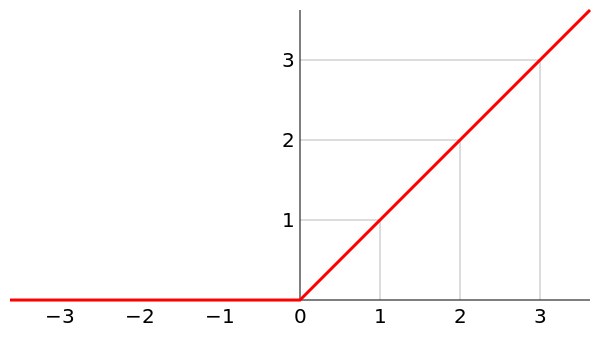
\includegraphics[width=0.8\linewidth]{figure/relu.png}
    \caption{ReLU}
    \label{fig:relu}
  \end{minipage}
\end{figure}

\paragraph{Regola di apprendimento delta} è basata sulla differenza tra il valore in uscita di riferimento e quello ottenuto dal modello e viene utilizzata per guidare la fase di apprendimento del modello stesso. Ogni volta che il valore in uscita viene calcolato il valore the peso del neurone viene corretto basandosi su una funzione di errore con l'obbiettivo di ridurre la differenza tra i due valori in esame. 

\paragraph{Retropropagazione dell'errore} conosciuta in inglese come backpropagation, è un algortimo per l'apprendimento supervisionato delle reti neurali artificiali basando sul gradiente discendente. Data una rete neurale ed una funzione di errore, il metodo calcola il gradiente della funzione riguardante i pesi della rete. È una generalizzazione della regola delta per i percetroni di reti multi livello a flusso avanti \cite{bp}.\\
La principale caratteristica di questa technica è che il gradiente procede all'indietro attraverso la rete, con il gradiente del livello finale calcolato prima di quello del primo livello. Questa soluzione permette un calcolo efficiente del gradiente per ciascuno dei differenti strati. L'algoritmo è strutturato nella seguente maniera:
\begin{enumerate}
  \item Calcolo errore per le unità di uscita
  \item Dal livello ppiù profondo, finchè il primo livello non viene raggiunto:
  \begin{enumerate}
    \item Propagazione dell'errore al precedente livello
    \item Aggiornamento dei pesi tra i due livelli
  \end{enumerate}
\end{enumerate}
La retropropagazione soffre del problema della vanificazione del gradiente, maggiore è il numero di livelli incorporati della rete maggiore sarà la difficoltà per l'allenamento della stessa. Per via della natura della retropropagazione, quando il valore in uscita viene generato, il peso dei neuroni viene aggiornato in accordo alla regola, mano a mano che l'algoritmo procede indietro il potere correttivo diminuisce, il relazione alla derivata della funzione di attivazione; in caso di reti superficiali il problema non si rivela così determinante, il processo avviene senza limitarne gli effetti. In caso di reti più profonde la problematica potrebbe diventare determinante. Una delle possibili soluzioni a questa problematica è l'impiego di funzioni di attivazione adatte, come la ReLU, la quale permette di alleggerire la problematica. Ulteriore soluzione è rappresentata dalla normalizzazione dei dati in ingresso, riscalando opportunamente i dati in entrata tra $[-1, 1]$ è possibile migliorare l'efficacia della procedura, questo perchè i dati verranno tenuti più lontani dagli estremi della funzione di attivazione. Esiste inoltre una tipologia di rete, memorie a lungo-corto termine, in inglese Long Short Term Memory (LSTM), sviluppata appositamente per mitigare il problema della vanificazione del gradiente nelle reti più profonde.

\paragraph{Reti neurali ricorsive} sono una classe di reti neurali che mantiene una connessione tra nodi e sequenze temporali. La principale differenza, rispetto le classiche reti neurali, sono connessioni di feedback, le quali permettono di mantenere traccia di dinamiche temporali. Questa tipologia di reti può processare singoli punti o intere sequenze di dati, come video e discorsi verbali, fondamentale la possibilità per gli step intermedi di mantenere informazioni di input precedenti senza definirne il numero a priori.\\
Questo tipo di strutture viene sfruttato per numerose applicazioni: classificazione di immagini, analisi sentimentale, traduzione macchina, classificazione video, ecc\dots

\paragraph{Memorie a lungo corto termine} le normali reti neurali possono correlare eventi a breve termine con il presente, in alcuni casi può essere sufficiente, in alcuni contesti invece può essere necessaria una connessione con margini più ampi, questo tipo di problematica viene tranquillamente gestito da questo tipo di reti. Cercando di effettuare una previsione sull'ultima parola di una frase tipo: "Il sole splende alto in \textit{cielo}" le parole precedenti all'ultima possono essere sufficienti a determinare un corretto suggerimento da parte della rete. In caso di frasi più complesse potrebbe essere necessaria una maggiore quantità di informazioni, per la frase: "Sono nato in Italia e parlo \textit{italiano}" il contesto si rivela fondamentale al fine di risolvere correttamente la problematica. In questa tipologia di situazione le reti LSTM possono essere di grande supporto.\\
Le reti a memorie a lungo e corto termine sono una tipologia speciale di reti ricorsive, introdotte da Hochreiter \& Schmidhuber (1997) \cite{lstm}, si sono rivelate sempre più utili in ambito previsionale, per la ricerca di schemi ricorrenti a livello temporale. Sono in grado di lavorare su una grandissima varietà di problemi differenti. Normalmente le reti ricorsive si prensentano su un singolo livello, in questo caso la struttura è più complessa ed è costituita da quattro diversi livelli, come visualizzato in figura \ref{fig:lstm}.

\begin{figure}[!ht]
  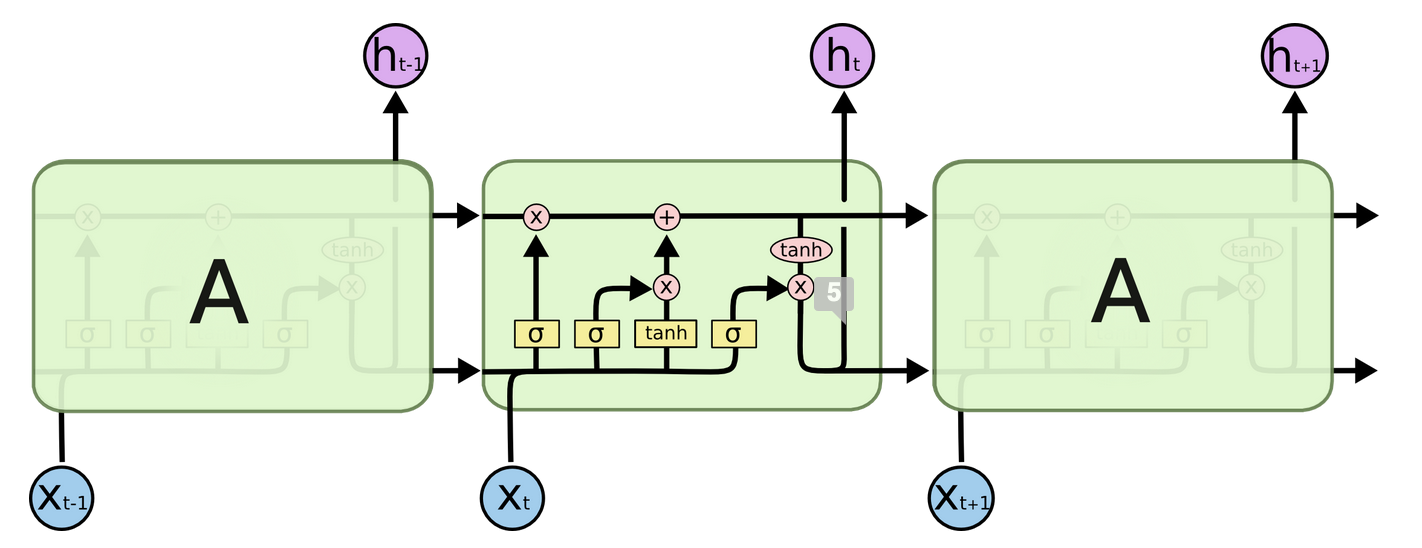
\includegraphics[width=\linewidth]{figure/lstm.png}
  \caption{Struttura rete LSTM \cite{lstm_image}}
  \label{fig:lstm}
\end{figure}

Il primo livello della rete ha il compito di filtrare i dati in input e selezionare cosa mantenere o meno, il secondo passaggio gestirà quali informazioni mantenere nello stato della cella. Il terzo livello invece ha il compito di aggiornare lo stato del nodo in base agli step precedenti. Lultimo livello si occupa invece della scelta del valore di uscita.

\section{Metriche di valutazione}
Ogni modello sviluppato necessità di essere valutato, ci sono innumerevoli modalità per valutare la bontà di un modello, ognuna con proprie caratteristiche. Ovviamente il parere più oggettivo si ottiene sfruttando espressione matematiche, sfortunatamente quest'ultime non sempre sono di facile e rapida comprensione da parte del l'uomo, alcuni errori come quello assoluto, quello relativo possono essere facilmente letti ed interpretati senza alcun tipo di problema; metriche come R2 o l'errore quadratico richiedono una valutazione più approfondita. Dopo attente valutazioni sono state definite alcune metriche che verranno utilizzate nella valutazione dei modelli, di seguito una breve trattazione matematica degli stessi.\\
La maggior parte degli errori deriva dal calcolo di errori più semplici, l'errore assoluto viene calcolato computanto la differenza tra l'obbiettivo $y$ ed il risultato ottenuto $x$:
\begin{center}
  \begin{equation}
    \epsilon = |y - x|
  \end{equation}
\end{center}
Oltre ad essere uno dei più semplici da calcolare risulta anche uno dei più semplici da comprendere in quanto permette di visualizzare direttamente lo scostamento rispetto al valore desiderato.\\
Una prima metrica derivata dall'errore assoluto è l'errore relativo, calcolato dividendo l'errore assoluto per il valore desiderato:
\begin{center}
  \begin{equation}
    \eta = \frac{\epsilon}{|x|} = \frac{|y - x|}{|x|}
  \end{equation}
\end{center}
Questo calcolo riscala direttamente il risultato tra [0, 1], ciò permette una migliore comprensione della differenza. Per esempio, con un valore desiderato di 530 ed un valore stimato di 570 i due errori vengono calcolati come segue:
\begin{center}
  \begin{equation}
      \epsilon = |520-570| = 50
  \end{equation}
  \begin{equation}
      \eta = \frac{50}{|520|} = 0.09
  \end{equation}
\end{center}
la differenza era di 50 un valore che potrebbe essere considerato elevato magari ma, rispetto al valore desiderato, l'errore è in realtà molto basso, circa 9\%. Gli errori presentati fino ad ora fungono da base per molti altri, esse infatti possono essere applicati solamente ad una coppia alla volta, i successivi, quelli realmente implementati invece possono essere applicati su un numero indefinito di valori.\\
L'errore medio assoluto (Mean Absolute Error, MAE) è il più semplice di quelli utilizzati ed è calcolato come la media di tutti gli errori assoluti:
\begin{center}
  \begin{equation}
    MAE = \frac{\sum_{i=1}^{n}{|y_{i} - x_{i}|}}{n} = \frac{\epsilon}{n}
  \end{equation}
\end{center}
Un altro utile metrica è derivata dall'applicazione dell'errore relativo alle misurazioni multiple, il calcolo dell'errore medio relativo, calcolato come la media di tutti gli errori relativi:
\begin{center}
  \begin{equation}
    REL = \frac{\sum_{i=1}^{n}{\frac{|y - x|}{|x|}}}{n}
  \end{equation}
\end{center}
L'impatto e l'immediatezza di questo valore permetto rapide valutazioni del comportamento generale del sistema. Per rendendere ancora più semplice la precisione del modello è si è deciso di definire il calcolo della precisione come:
\begin{center}
  \begin{equation}
    ACC = 1 - REL
  \end{equation}
\end{center}
L'ultimo errore calcolato è rappresentato da R2, conosciuto anche come coefficiente di determinazione, un dato molto più complesso da comprendere, utilizzato nella valutazione della bontà della curva nella regressione lineare, calcola una proporzione tra la variabilità dei dati e la precisione del modello statistico applicato, più nello specifico calcola la frazione della varianza della variabile dipendente espressa dalla regressione.\\
La formulazione del coefficiente è la seguente:
\begin{center}
  \begin{equation}
    R^2 = \frac{ESS}{TSS} = 1 - \frac{RSS}{TSS}
  \end{equation}
\end{center}
dove, con $y_i$ i dati osservati, $\bar{y}$ la loro media e $\hat{y_i}$ i dati ottenuti dal modello:
\begin{center}
  \begin{equation}
    ESS = \sum_{i=1}^{n}(\hat{y_i} - \bar{y})^2
  \end{equation}
\end{center}
rappresenta la devianza spiegata dal modello. Mentre:
\begin{center}
  \begin{equation}
    TSS = \sum_{i=1}^{n}(y_i - \bar{y})^2
  \end{equation}
\end{center}
è la devianza totale, e:
\begin{center}
  \begin{equation}
    RSS = \sum_{i=1}^{n}e_i^2 = \sum_{i=1}^{n}(y_i - \hat{y_i})^2
  \end{equation}
\end{center}
la varianza residua.\\
In generale il valore di R2 è compreso tra [0, 1], tanto più il valore è prossimo a 1, tanto meglio il modello segue i dati e viceversa se tende a zero.

% #######################################
% #           Pre-processing            #
% #######################################

\chapter{Pre-elaborazione}
\label{chap:preprocessing}
La fase di pre-elaborazione dei dati è fondamentale nell'applicazione di algoritmi statistici. L'utilizzo di dati non attentamente valutati può generare inutile rumore all'interno del modello sviluppato. Questa fase non si occupa solamente di rimuovere i dati inutili o sporchi, ma si occupa anche di estrarre informazioni derivate, ovvero non direttamente presenti nella base dati, e di aggregarli in maniere efficiente in modo da guidare più correttamente il sistema. 

\section{Pulizia}
Il primo step di questa importante fase riguarda l'estrazioni dei dati dalla loro sorgente. Come anticipato nel capitolo \ref{chap:dataset} i dati sono salvati all'interno di un file SQLITE, una gestore SQL offline. Ogni singolo progetto: hadoop, cassandra, ecc... È salvato all'interno di uno specifico file con il nome del progetto seguito da .sqlite. La logica di interazione con questa sorgente è basata su SQL e segue tutte le classiche procedure ad esso correlate. Al fine di automatizzare questa procedura verranno sfruttate le librerie open source sviluppate per l'interfacciamento tra Python ed i sistemi SQLITE.\\
L'estrazione di informazioni e l'aggregazione verranno gestite principalmente all'interno dello script Python, esclusi pochi casi le query applicate saranno sufficientemente semplici. L'elaborazione di tutti questi dati è stata demandata a Pandas, di conseguenza, i risultati di ogni query verranno caricati all'interno di DataFrame di Pandas per una rapida ed efficiente gestione successiva.\\
Rispetto al repository di GitHub, questa fase, viene gestita dal sotto-progetto DataAnalysis\_Issue, tramite lo script:
\begin{lstlisting}[language=Python, frame=single]
  thesisProjectJN/DataAnalysis_Issue/main.py
\end{lstlisting}
Prima di poter procedere direttamente con l'estrazione delle informazioni è stata necessaria una analisi dei dati. La natura open source di questi progetti prevede il mantenimento e lo sviluppo da parte della communità pubblica, questo comporta potenzialmente un numero di sviluppatori infinito, chiunque infatti potrebbe partecipare allo sviluppo del progetto. Vista la rilevanza del progetti in questione, lo sviluppo, nonostante sia stato mantenuto open, viene regolarmente sostenuto da società e fondazione che ne fanno utilizzo nei loro software interni, hadoop, per esempio, viene regolarmente mantenuto e sponsorizzato da Google. Questo contributo è chiaramente fondamentale per l'avanzamento del progetto, una disponibilità economica permette di allocare sviluppatori direttamente al progetto, senza che però esso venga privatizzato. I progetti in esame fanno tutti parte di questo caso, la motivazione principale di questa scelta ricade sulla differente gestione dello sviluppo, una costante e regolare progettazione permette di generare una reportistica più precisa e fruibile dai sistemi di statistica. L'origine open di questi progetti porta un ulteriore vantaggio, essendo fruibili da tutti, una maggiore quantità di interessati ne potranno fruire, essendo una comunità specifica, chi farà utilizzo di tale progetti facilmente si impegnerà anche nel segnalare errori e malfunzionamenti dello stesso permettendo una efficiente gestione delle problematiche. Chiaramente la segnalazione di questa anomalie sarà gestita in maniera prefissata con la compilazione di appositi form, griglie di valutazione e tante altre informazioni strutturare le quali andranno a fare della nostra analisi. Tutte queste caratteristiche si rivela di gran supporto alla causa, sfortunatamente però sono anche fonte di problematiche che, in progetti privati, non emergerebbero. Un utente che non si occupa direttamente dello sviluppo di un progetto potrebbe andare a riportare una problematica in modo erroneo, per esempio, ciò che un utilizzatore potrebbe riportare come un errore del sistema in realtà si potrebbe rivelare un errore nell'utilizzo dello dello stesso, tutto ciò andrebbe ad aggiungere disturbo alla nostra analisi. Valutando per esempio la durata in giorni delle issue, riporta in figura \ref{fig:day_duration}, si può facilmente evincere come i valori siano mal distribuiti, il numero di issue aperte e chiuse nel giro di 48 ore è elevatissimo, circa il 20\% del totale, questo per quanto riportato sopra.
\begin{figure}[!ht]
  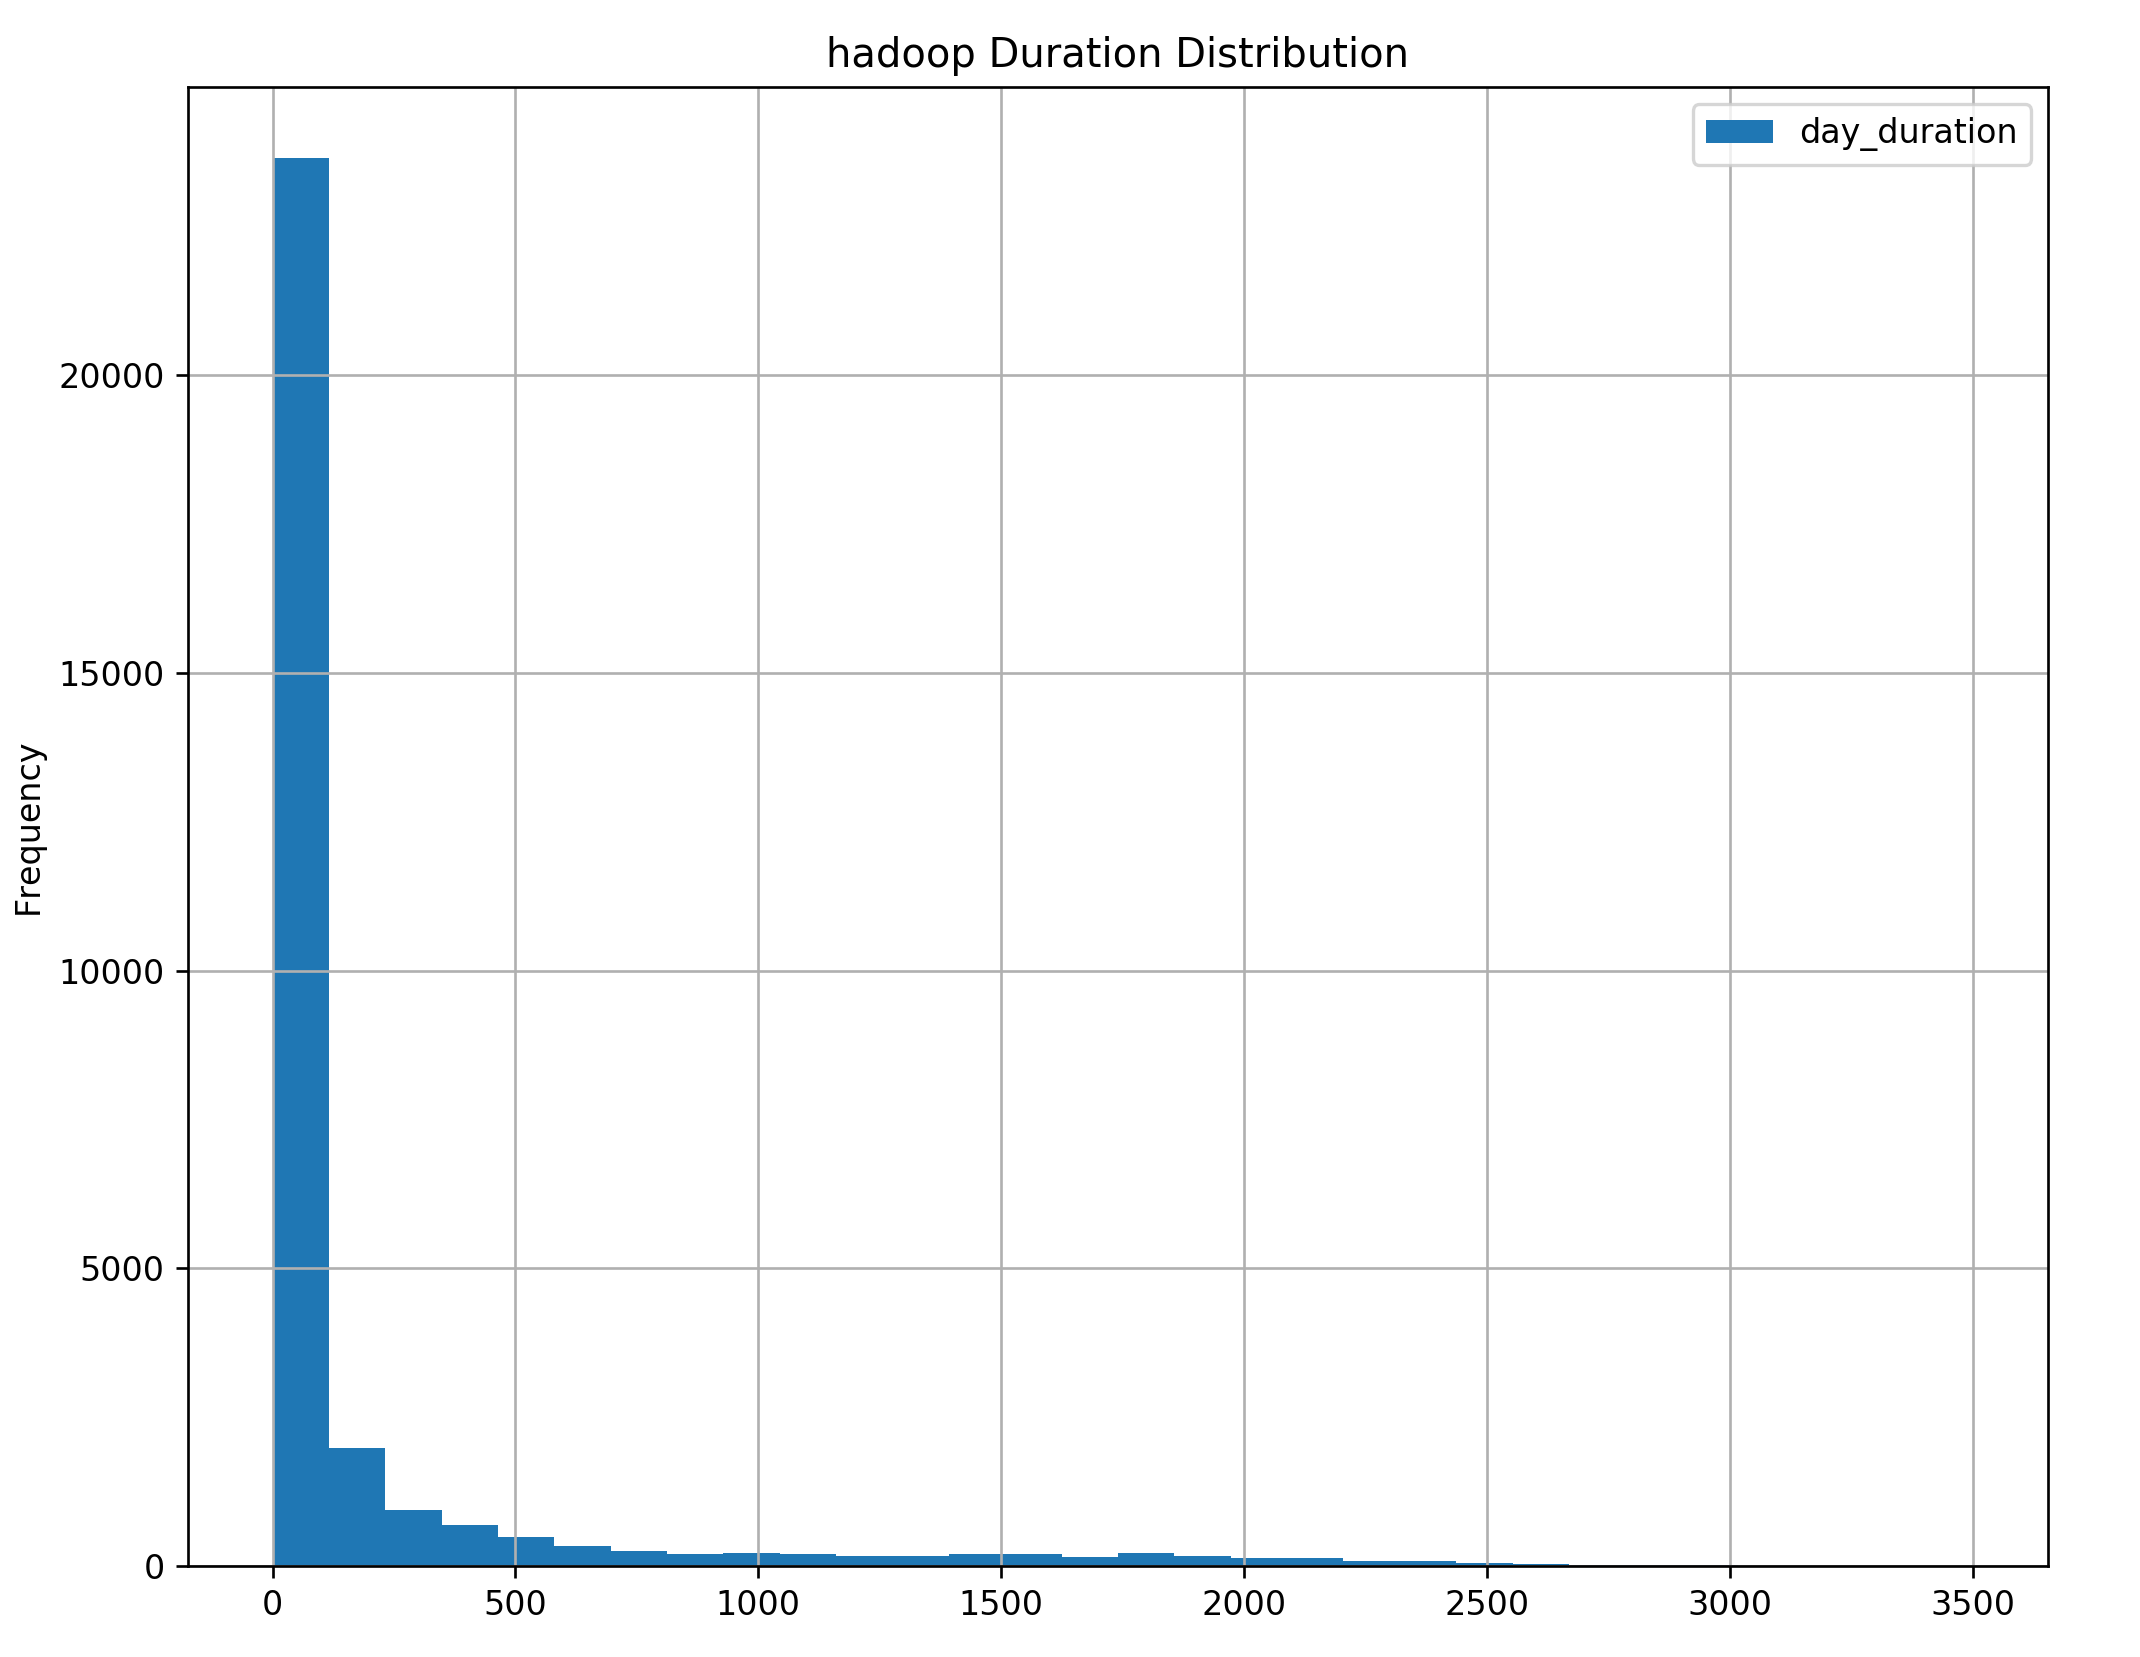
\includegraphics[width=\linewidth]{figure/day_duration.png}
  \caption{Distribuzione della durata in giorni delle issue}
  \label{fig:day_duration}
\end{figure}
La figura \ref{fig:d48h_duration} visualizza le circa 8000 di 39000 issue aperte risolte nelle prime 48 ore dalla loro apertura.
\begin{figure}[!ht]
  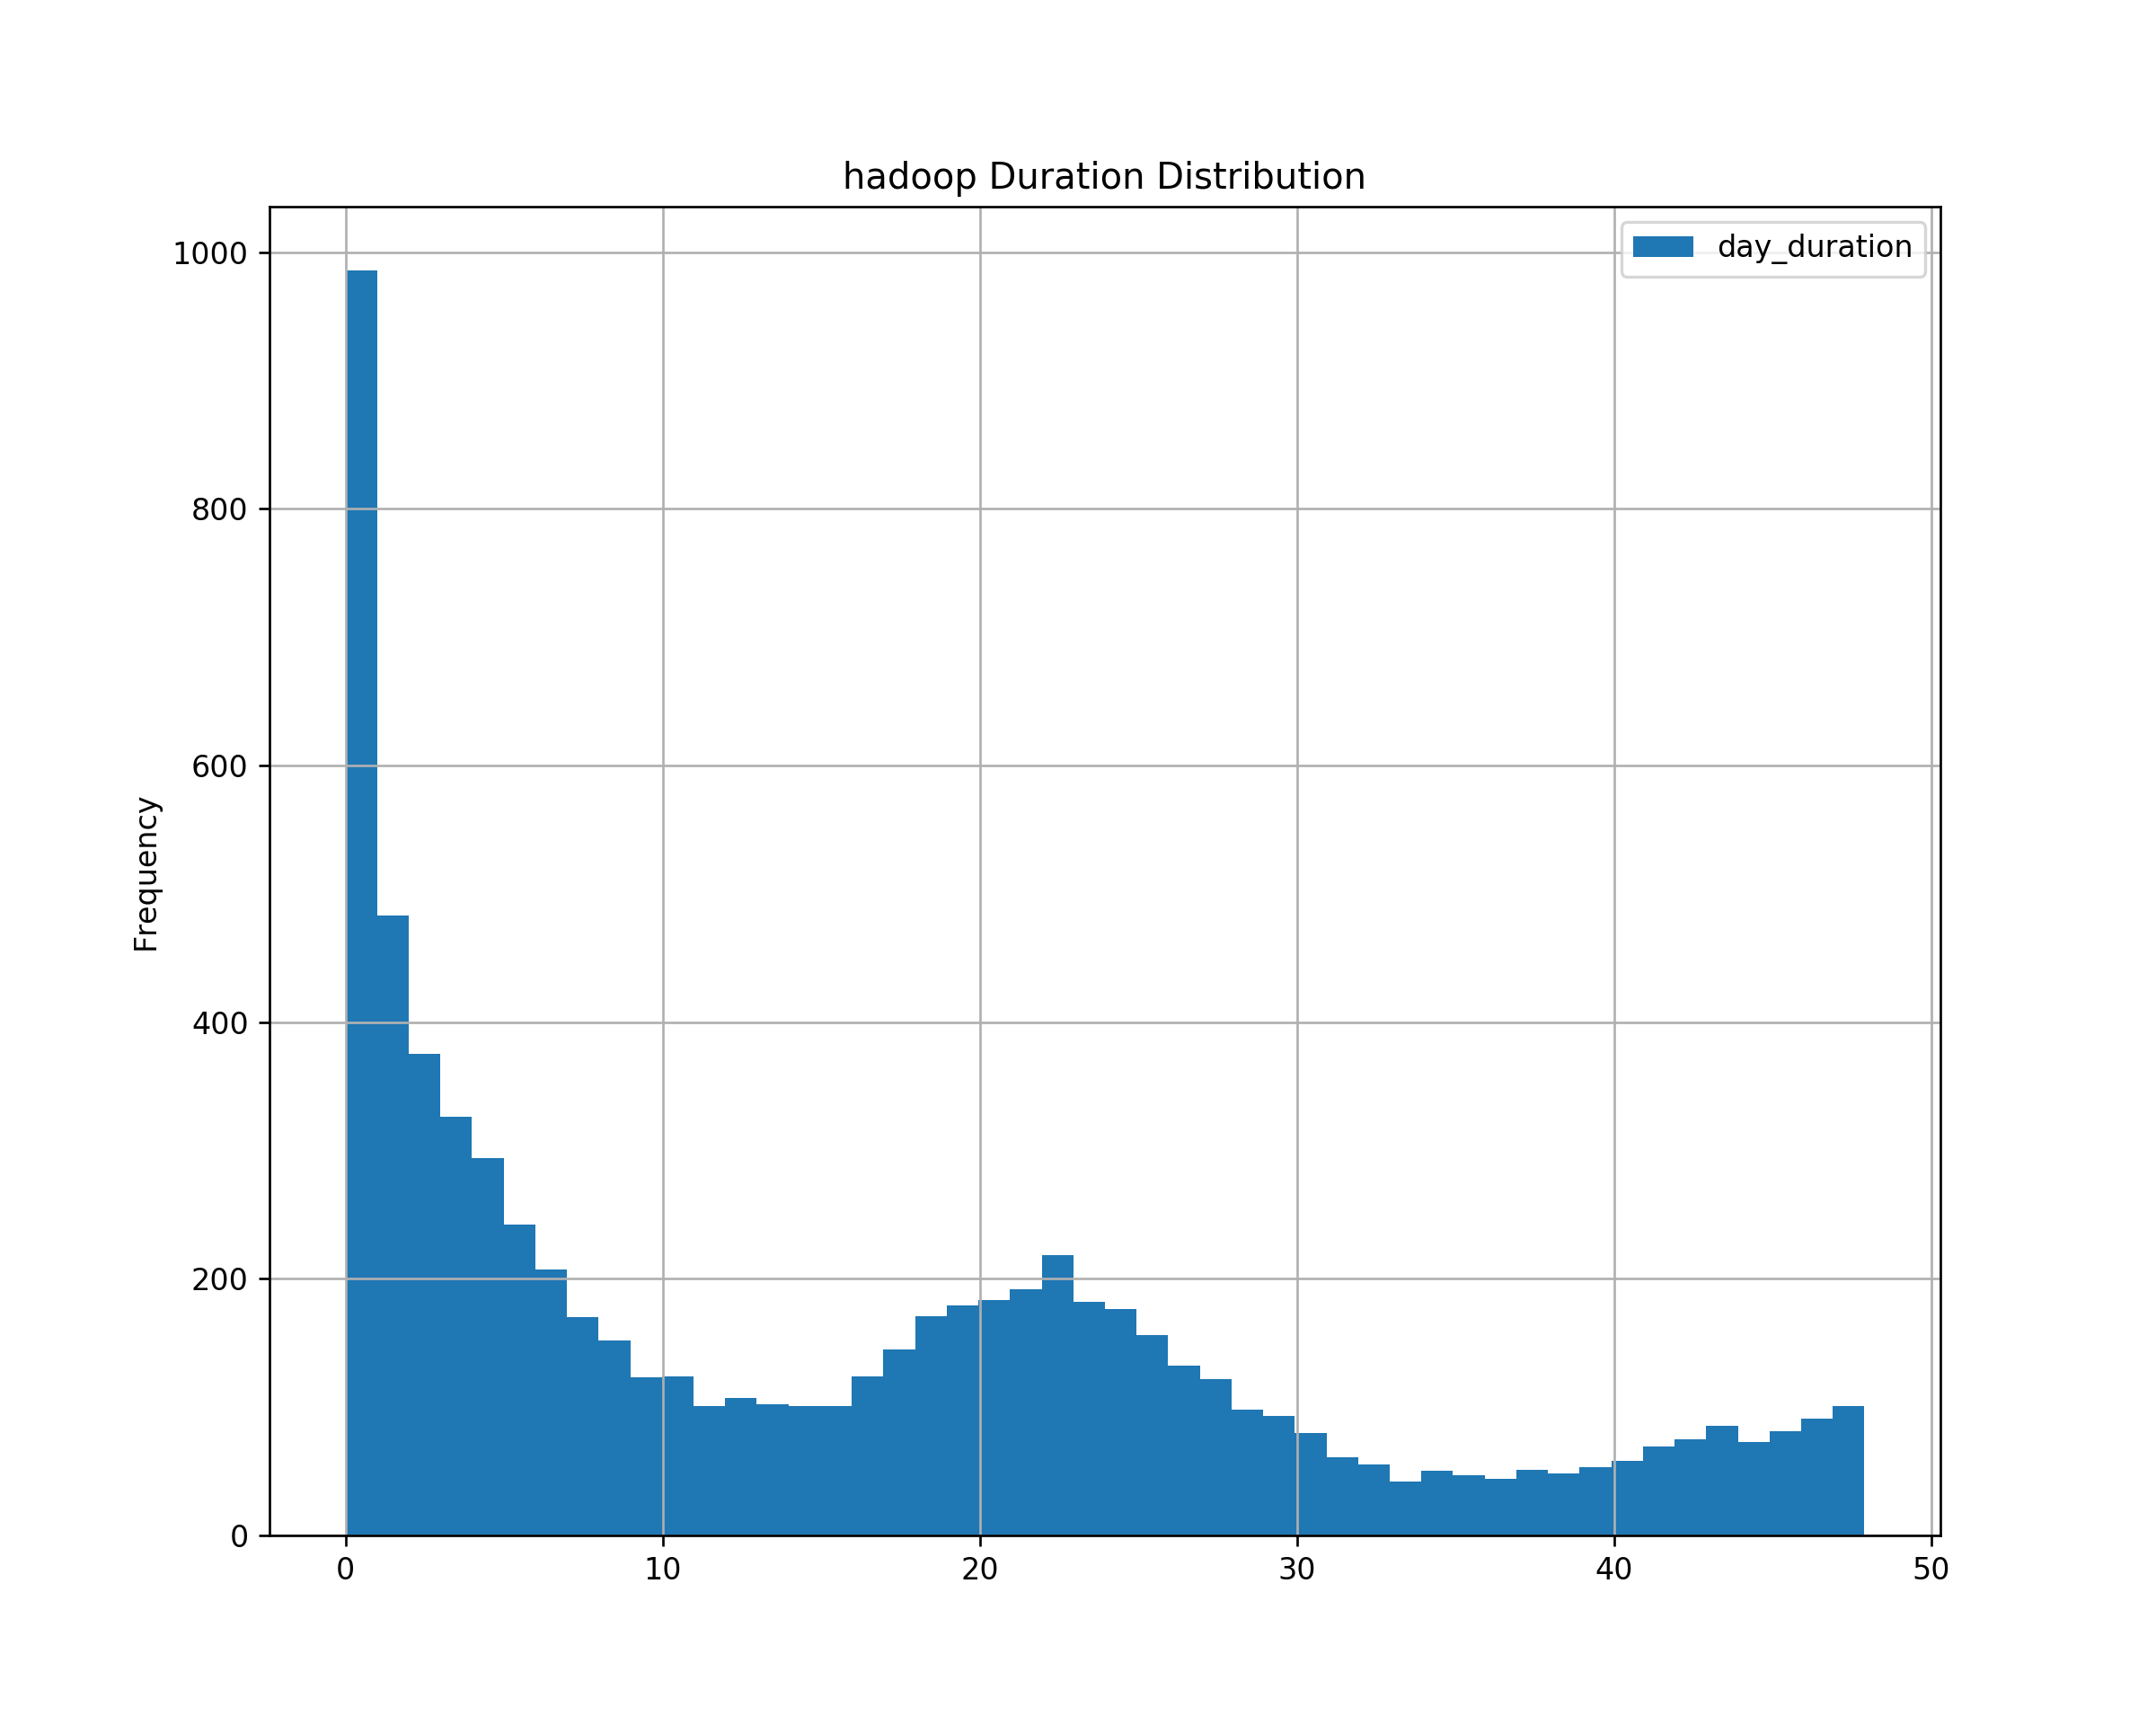
\includegraphics[width=\linewidth]{figure/48h_duration.png}
  \caption{Distribuzione della durata in ore nelle prime 48h}
  \label{fig:d48h_duration}
\end{figure}
Altra grande problematica è costituita da issue che non hanno avuto nessuna data di chiusura, non sempre è possibile risolvere una issue, ma spesso non è un problema di risoluzione quanto un problema di comprensione del problema. I canoni dello sviluppo richiedono che ogni problematica venga risolta prima della consegna della versione definitiva, questo significa che tutte le issue vanno risolte. Per evitare quindi di aggiungere rumore ai nostri dati si è deciso di considerare solamente le problematiche risolte perchè le uniche realmente di valore all'interno del processo di sviluppo. Sono stato considerati quindi solo in casi in cui il campo status è stato marcato con \textit{closed} o \textit{Resolved} e il campo resolution a \textit{fixed}.
Ulteriore filtro è stato posto sulla tipologia di problematica riportata, sono stati considerati solamente le issue marcate con il type \textit{Bug}, si è analizzato come molte delle altre etichette vengano spesso posticipate portando a tempi di risoluzione veramente poco sensati. Tutti questi filtri, riassunti nel seguente pezzo di codice:
\begin{lstlisting}[language=Python, frame=single, basicstyle=\small]
  def filter2(df_init):
    df = df_init.copy()
    df = df[(df['type'] == 'Bug')]
    df = df[(df['close_dt'].isna() == False)]
    df = df[((df['status'] == 'Closed') 
                & (df['resolution'] == 'Fixed')) 
              | ((df['status'] == 'Resolved') 
                & (df['resolution'] == 'Fixed'))]
    return df
\end{lstlisting}
hanno portato una riduzione del circa 60\% del numero di issue, passando quindi da 30000 a circa 10000. Questa riduzione non ha portato sbilanciamenti tra gli altri parametri.\\
Il rilascio di un progetto è normalmente strutturato in versioni, solitamente catalogato tra major e minor, nella preparazione di questi dati si è optato per la divisione in versioni dei singoli file, ciò permetterà successivamente di gestire la fase di allenamento in diverse mdalità, come vedremo nel capitolo \ref{chap:forecasting}. In figura \ref{fig:hadoop_release_split} è possibile visualizzare il conteggio di issue attive, ovvero ancora da risolvere quindi aperte, lungo il periodo di tutte le versioni con la loro differente allocazione temporale lungo tutto il periodo dello sviluppo.\\
\begin{figure}[!ht]
  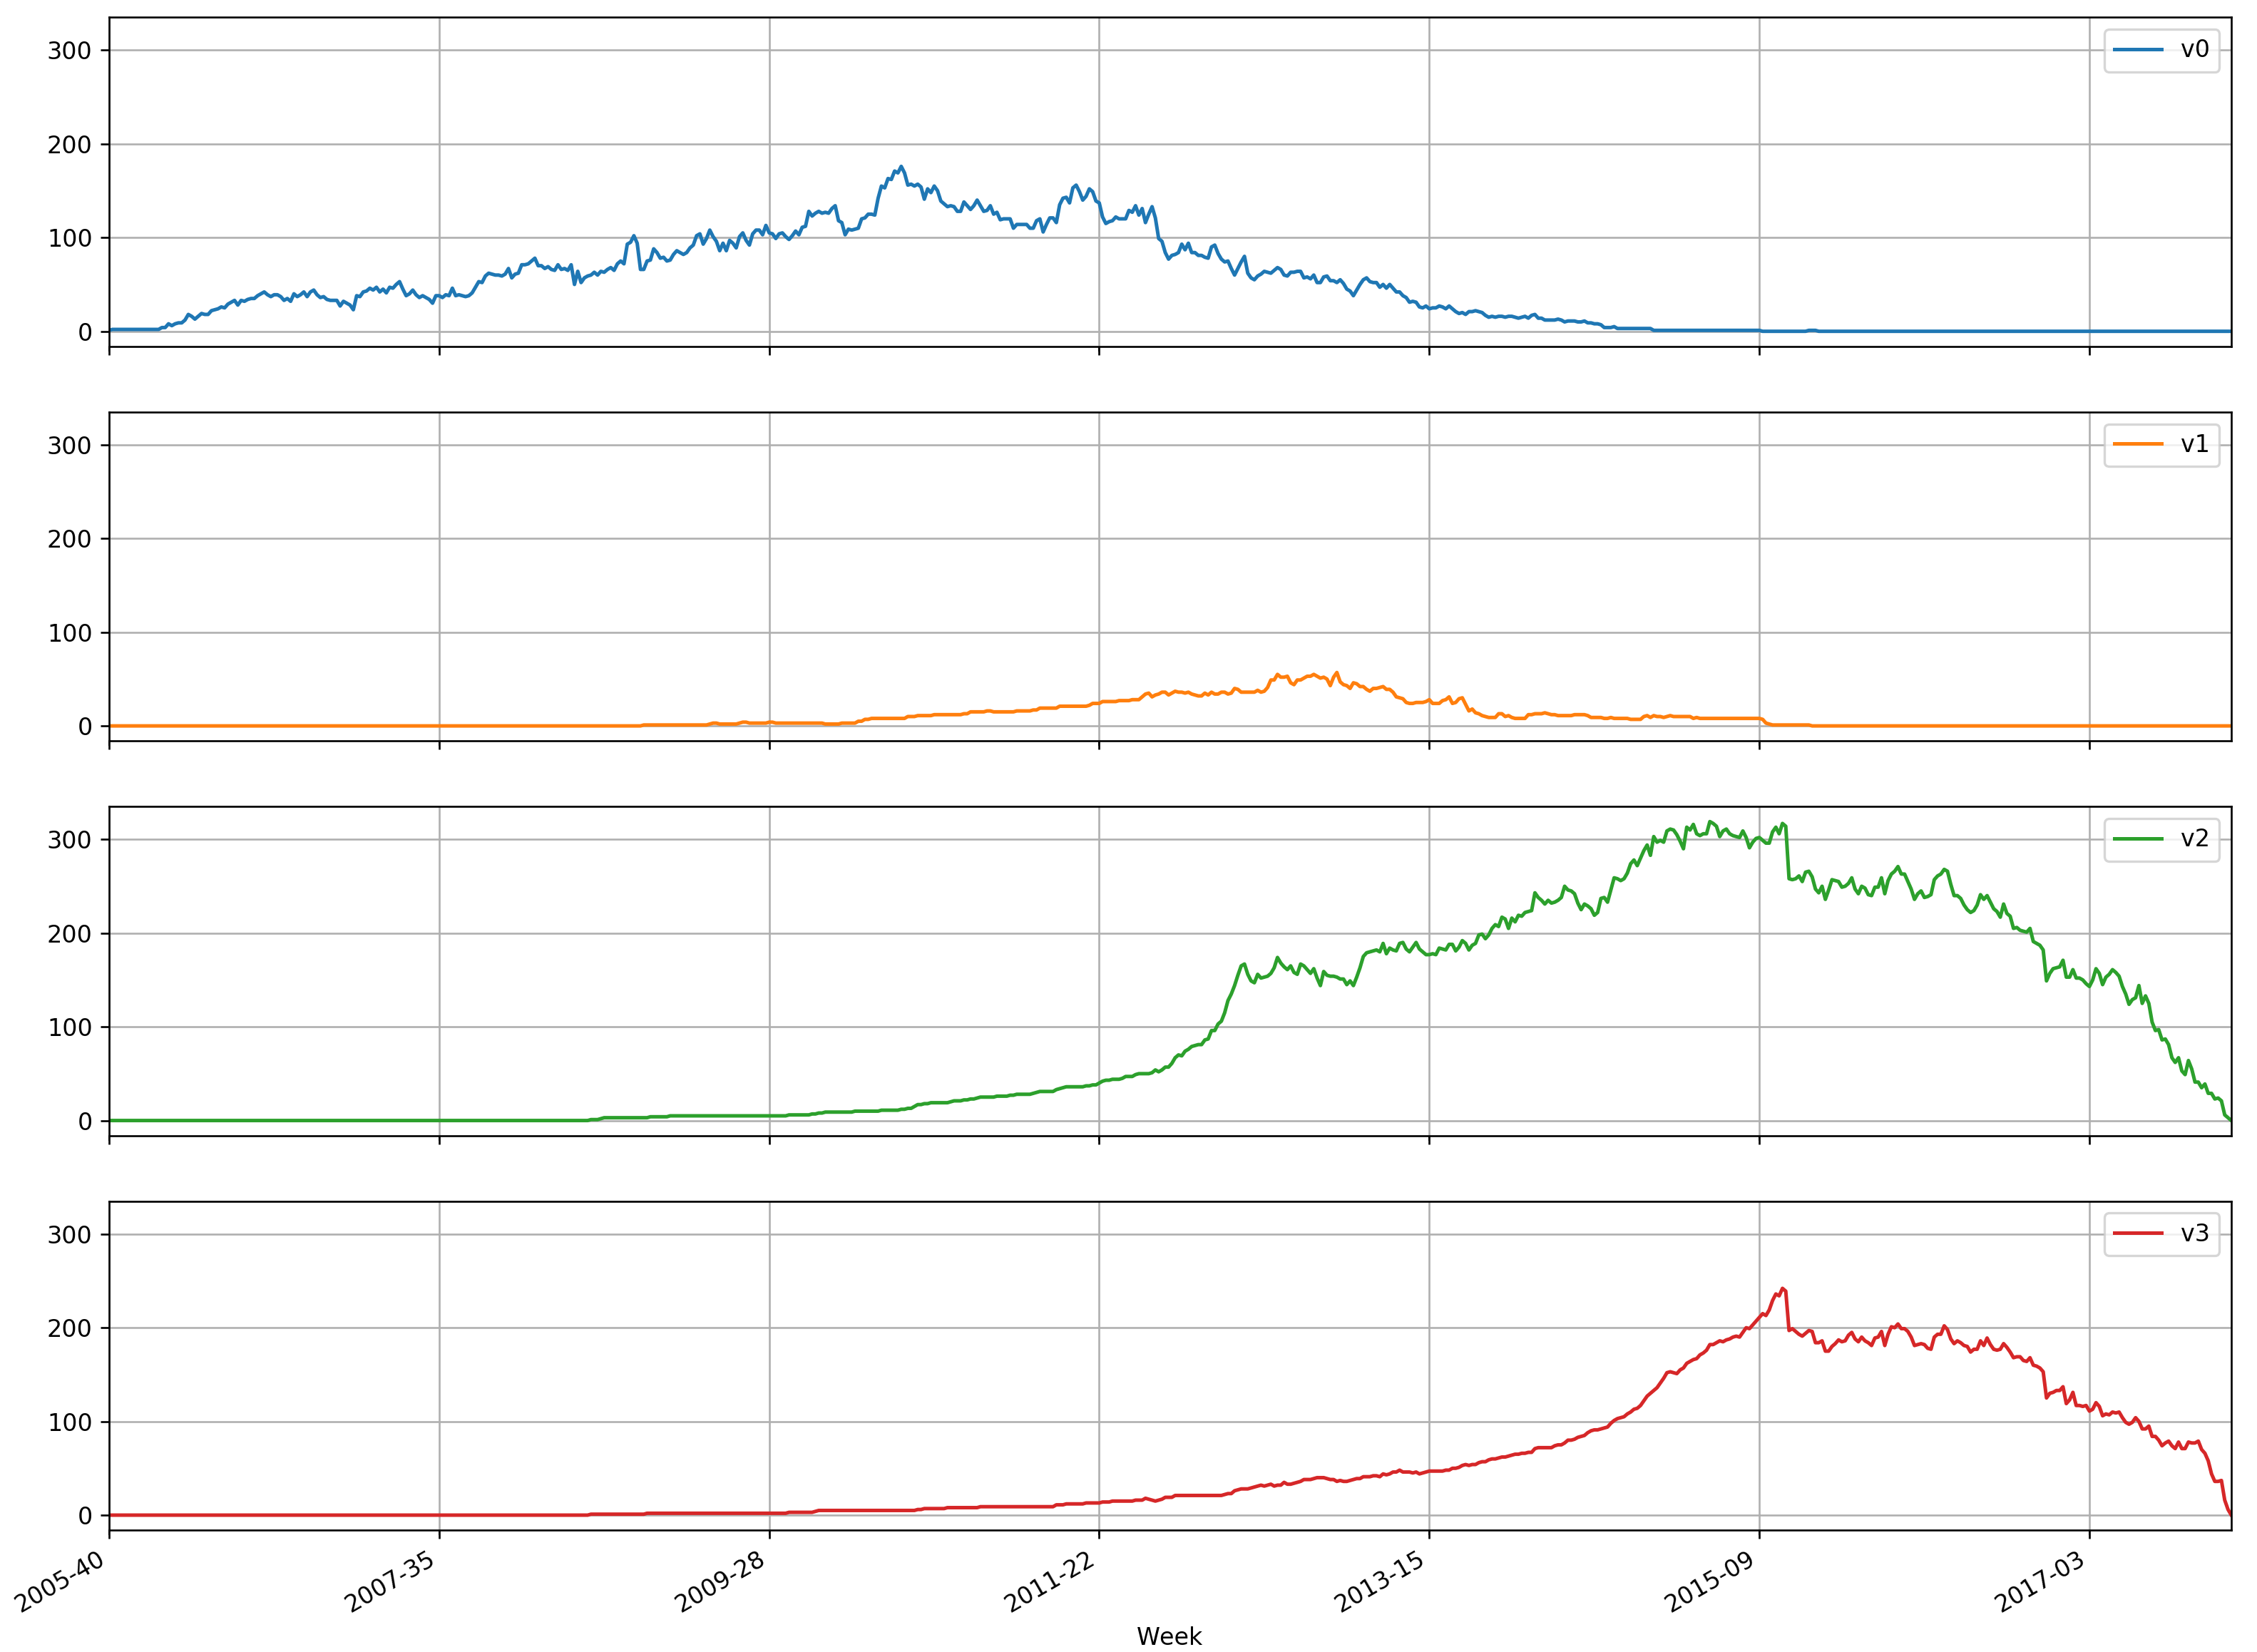
\includegraphics[width=\linewidth]{figure/hadoop_release_split.png}
  \caption{Conteggio del numero di issue attive per ogni versione}
  \label{fig:hadoop_release_split}
\end{figure}
L'ultimo step fondamentale, distribuito in vari punti a livello di processo, è quello riguardante l'aggregazione dei dati. I dati all'interno della base dati non hanno una organizzazione temporale, l'unità centrale di tutto è la singola issue, chiaramente le informazioni temporali sono presenti, sia di apertura che di chiusura. L'utilizzo dei dati in questa forma era inconcludente, senza distribuzione temporale le fasi di rilascio di nuove versioni o di grossi errori introdotti poterebbero a picchi e false informazioni a livello di dati. Dopo attenta analisi riguardanti durata, tipologia e distribuzione si è optato per l'aggregazione settimana-anno, questa opzione è stata scelta in modo da limitare i problemi dell'analisi giornaliera con conseguente aumento dei dati, senza però perdere tutte le informazioni in caso di aggregazione più elevata come quella mensile. Questa aggregazione ha permesso pure di risolvere il problema della settimana lavorativa, così facendo i giorni feriali non generano problematiche. Mantenere, oltre alla settimana, l'anno permette di avere una distribuzione temporalmente sensata, senza la sovrapposizione di dati ed informazioni. Chiaramente i differenti orizzonti di previsione saranno gestiti a livello settimanale.\\

La funzione implementante tutte le scelte descritte in questo paragrafo è la seguente:
\begin{lstlisting}[language=Python, frame=single, basicstyle=\small]
  def version_forecast_file(dataset)
\end{lstlisting}
l'esecuzione di essa permetterà di estrarre file per ogni versione e per ogni finestra temporale definita.

\section{Estrazioni base}
Il primo step di questa procedura utilizza la query più complessa e si occuperà dell'estrazioni di molti parametri, già parzialmente aggregati che verranno utilizzati successivamente per l'estrazioni di informazioni più complesse.\\
La funzione \textit{make\_component\_change\_clean(dataset)} dello script ha il compito, attraverso una serie di query annidate di estrarre alcuni dati utili alla generazione dei file finali. Nello specifico i parametri estratti saranno:
\begin{itemize}
  \item Data di modifica
  \item Componente interessato dalla modifica
  \item Linee variate (differenza tra aggiunte/rimosse/modificate)
  \item Numero di commit
  \item Resolution
  \item Status
  \item Effort
\end{itemize}
Tutti questi parametri verranno successivamente utilizzati per estrarre informazioni più complesse. Il parametro effort invece, calcolato come:
\begin{center}
  \begin{equation}
    \textrm{effort} = \textrm{authors} * 0.8 + \textrm{commit\_count} * 0.15 + |\textrm{line\_change}| * 0.05
  \end{equation}
\end{center}
è stato estratto ma poi successivamente scartato perchè poco esplicativo del lavoro realmente necessario nella risoluzione della problematica emersa. L'eliminazione di grossi file portava ad un enorme sbalzo nel numero di linee modificate.\\

L'estrazione più grande viene effettuata tramite la query:
\begin{lstlisting}[language=SQL, frame=single, basicstyle=\small]
  SELECT * 
  FROM issue, issue_fix_version
  WHERE issue.issue_id = issue_fix_version.issue_id 
          AND fix_version LIKE '{}%' 
\end{lstlisting}
questa estrazione verrà poi filtrata secondo le precedenti disposizioni, verrà inoltre utilizzata come base per la creazione del DataFrame temporale, tramite la sua minore e la sua massima data presente. Nonostante l'elevato numero di informazioni, a seguito del filtraggio del dati, non tutte le settimane presentavano variazioni di problematica attive, per questo motivo è stato necessario effettuare una unione tra il DataFrame contenente tutte le issue ed un ulteriore DataFrame generato partendo dalla prima data e arrivando fino all'ultima data contenuta nel DF issue. Così facendo si è potuto ottenere un set con le informazioni distribuite su un lasso di tempo continuo e senza passaggi mancanti, il codice utilizzato è il seguente:
\begin{lstlisting}[language=Python, frame=single, basicstyle=\small]
  # GET ALL THE WEEK IN THE TIME SLICE
  min_date = issue['open_dt'].min().date()
  max_date = issue['close_dt'].max().date()
  
  all_date = pd.date_range(start=min_date, end=max_date,
                            freq='D')
  all_date = pd.DataFrame(all_date)

  all_date['w'] = all_date[0].dt.strftime('%Y') 
                  + '-' 
                  + all_date[0].dt.strftime('%W')

  all_date = all_date.drop([0], axis=1)
  all_date = all_date.drop_duplicates(keep='last')
\end{lstlisting}

\section{Estrazioni complesse}
Alcune delle informazioni utilizzate dal nostro modello necessitano di un processo di estrazione più complicato, suddiviso sia in una parte a livello DB sia in parte a livello script Python.
\paragraph{Borsa di parole componenti modificati} alla base dell'apertura di una issue vi è una motivazione, il modulo per riportare queste problematiche è solitamente predefinito in modo da guidare più facilmente lo sviluppatore e permettergli di riprodurre la problematica. Una volta trovata la problematica è buona norma segnalare il componente o comunque circoscrivere la problematica ad una zona e non a tutto il progetto. La base dati utilizzata presenta una tabella, direttamente collegata a quella delle issue, con il nome \textit{issue\_component}. Questa tabella correla la issue direttamente ad un componente del progetto. Una delle feature estratte si basa proprio su questa connessione, si è deciso di aggiungere una serie di informazioni legate ai componenti più utilizzati ed il numero di issue facenti riferimento ad esso per ogni settimana. Queste informazioni sono state ottenute sfruttando le borse di parole, bag of words in inglese, una tecnica molto usata nell'elaborazione del linguaggio naturale. La tecnica permette di tenere traccia di parole e la loro frequenza respetto un qualsiasi tipo di aggregazione. Nel nostro caso i file verranno strutturati nel seguente modo, oltre a presentare le varie informazioni, vi saranno al più dieci colonne facenti riferimento ai dieci componenti più utilizzati dove, per ogni riga verrà rappresentato il numero di volte in cui quel componente è stato considerato parte della issue per quella settimana. La tabella \ref{tab:bag_word} esemplifica il concetto esposto.
\begin{center}
  \captionof{table}{Borsa di parole} \label{tab:bag_word}
  \begin{tabular}{ |c|c|c|c|c|c|c| }
     \hline
     \textbf{week} & \textbf{...} & \textbf{security} & \textbf{fs} & \textbf{hdfs} & \textbf{fs-s3} & \textbf{...} \\
     \hline
     \hline
     04-2017 & ... & 1 & 5 & 0 & 0 & ...\\
     \hline
     05-2017 & ... & 0 & 2 & 1 & 1 & ...\\
     \hline
     06-2017 & ... & 3 & 0 & 0 & 8 & ...\\
     \hline
     07-2017 & ... & 2 & 0 & 1 & 6 & ...\\
     \hline
  \end{tabular}
\end{center}
Il processo di estrazione di queste informazioni è stato effettuato utilizzando una funzionalità della libreria di Sci-Kit, CountVectorize, il processo svolto come segue:
\begin{lstlisting}[language=Python, frame=single, basicstyle=\small]
  def word_recognition(df_cols):
    additional = frozenset()
    stop_words = text.ENGLISH_STOP_WORDS.union(additional)
    vect = CountVectorizer(lowercase=True, 
                            preprocessor=None, 
                            analyzer='word', 
                            stop_words=frozenset(stop_words),
                            max_features=max_features)
    X = vect.fit_transform(df_cols)
    return pd.DataFrame(X.todense(), 
                          columns=vect.get_feature_names())
\end{lstlisting}
si occupa di rimuovere, nel caso in cui siano prensenti, tutte le stop word ovvero quelle parole che vogliamo filtrare prima che vengano trattate dal sistema, esisto molti dizionari già presenti, è possibile personalizzarli. Successivamente calcolerà la frequenza di ogni parola e tramite apposite trasformazioni sarà possibile ottenere le colonne come visualizzato in tabella.\\
L'inserimento di tutte queste informazioni tuttavia non ha introdotto grandi vantaggi in termini di risultati addirittura, in alcuni casi, si è rivelata negativa. In qualsiasi caso è stata una opzione interessante da valutare, la sorgente dei problemi poteva proabilmente essere collegata alla difficolta di risoluzione degli stessi, proabilmente in progetti più piccoli questo parametro può rivelarsi più importante.

\paragraph{Seniority} facilmente traducibile come esperienza dello sviluppatore, è una informazione aggregata che ha lo scopo di definire l'esperienza, relativa al progetto, di uno specifico sviluppatore. Per ogni issue risolta corrisponde uno o più commit, ogni commit ovviamente viene eseguito da uno sviluppatore, ogni sviluppatore ha iniziato ad occuparsi del progetto a partire da una specifica data, nel nostro caso si è scelta la data del primo commit. Combinando opportunamente queste informazioni tra di loro è stato possibile definire questo valore nominato seniority. L'idea alla base è che ogni sviluppatore, mano a mano che si occupa del progetto, oltre a maturare una certa esperienza personale, matura anche una esperienza specifica del progetto, conseguentemente dovrebbe essere per lui più semplice individuare e risolvere i problemi. La feature creata correla il momento temporale dello sviluppo con la seniority a quel tempo di quel preciso sviluppatore. Chiaramente questo processo è sensato fintanto che il contributo da parte dello sviluppatore è costante, i contributori del mondo open source vengono quindi facilmente trascurati in questo conteggio.\\
Una volta estratti tutti i dati necessari e calcolata la seniority vera e propria viene aggregata per settimana prima di essere unita al resto delle informazioni già esistenti. La computazione vera e propri è semplice ed, somma in maniera pesata il numero di giorni dal primo commit al numero di commit effettuati.\\
L'aggiunta di questo parametro non ha portato molte variazioni durante la previsione.

\paragraph{Severity} il presente elaborato cerca di sviluppare un modello statistico in grado di prevedere l'andamento di un fenomeno nel tempo. Il fenomeno in esame dovrebbe descrivere l'andamento della difettosità. Occorrere chiararire questo concetto, il termine difettosità, scelto per la sua brevità, non è un semplice valore rappresentante il mero conteggio delle problematiche attive in uno specifico momento dello sviluppo, rappresenta molto di più quasi come se fosse una sorta di sforzo necessario al fine di riuscire correttamente a risolvere la problematica. Per poter meglio comprendere la questione è necessario capire come viene calcolata.\\
Ogni issue è caratterizzata da una etichetta di \textit{priority}, come già accennato nel capito \ref{chap:dataset}, queste cinque etichette: \textit{critical}, \textit{major}, \textit{blocker}, \textit{minor} e \textit{trivial} dovrebbero rappresentare la priorità, assegnata dallo sviluppatore che sta gestendo la richiesta. Inizialmente si era optato per definire questi valori a tavolino senza nessuna valutazione, i valori, ordinati per priorità erano rispettivamente:
\begin{center}
  \captionof{table}{Valori numeri priorità} \label{tab:priority}
  \begin{tabular}{ |c|c|c|c|c| }
     \hline
     \textbf{Critical} & \textbf{Major} & \textbf{Blocker} & \textbf{Minor} & \textbf{Trivial} \\
     \hline
     \hline
     50.0 & 10.0 & 2.00 & 1.00 & 0.50 \\
     \hline
  \end{tabular}
\end{center}
Le performance del modello erano comunque elevate. La ricerca a livello di letteratura non ha avuto grande riscontro, queste etichette, se ben molto comuni non sono standard quindi non sempre vengono utilizzate in questo modo. Oltretutto questa base dati non presenta nessuna ricerca correlata, ad oggi, quindi non vi sono nemmeno valori di confronto.\\
Una più attenta, seppur semplice, valutazione ha permesso di notare come non vi fosse una grandissima correlazione tra tempo di risoluzione e priorità della issue, si è deciso quindi di optare per una differente traduzione della etichetta. Si è deciso di scegliere il valore dinamicamente per ogni progetto, usando il valore medio della distribuzione, per ogni etichetta, del tempo di risoluzione della issue. Prendendo in esame il progetto \textit{hadoop}, le distribuzioni di ciascuna etichetta sono visualizzate in figura \ref{fig:duration_distr}, nel titolo viene anche visualizzato il valor medio della distribuzione.
\begin{figure}[!ht]
  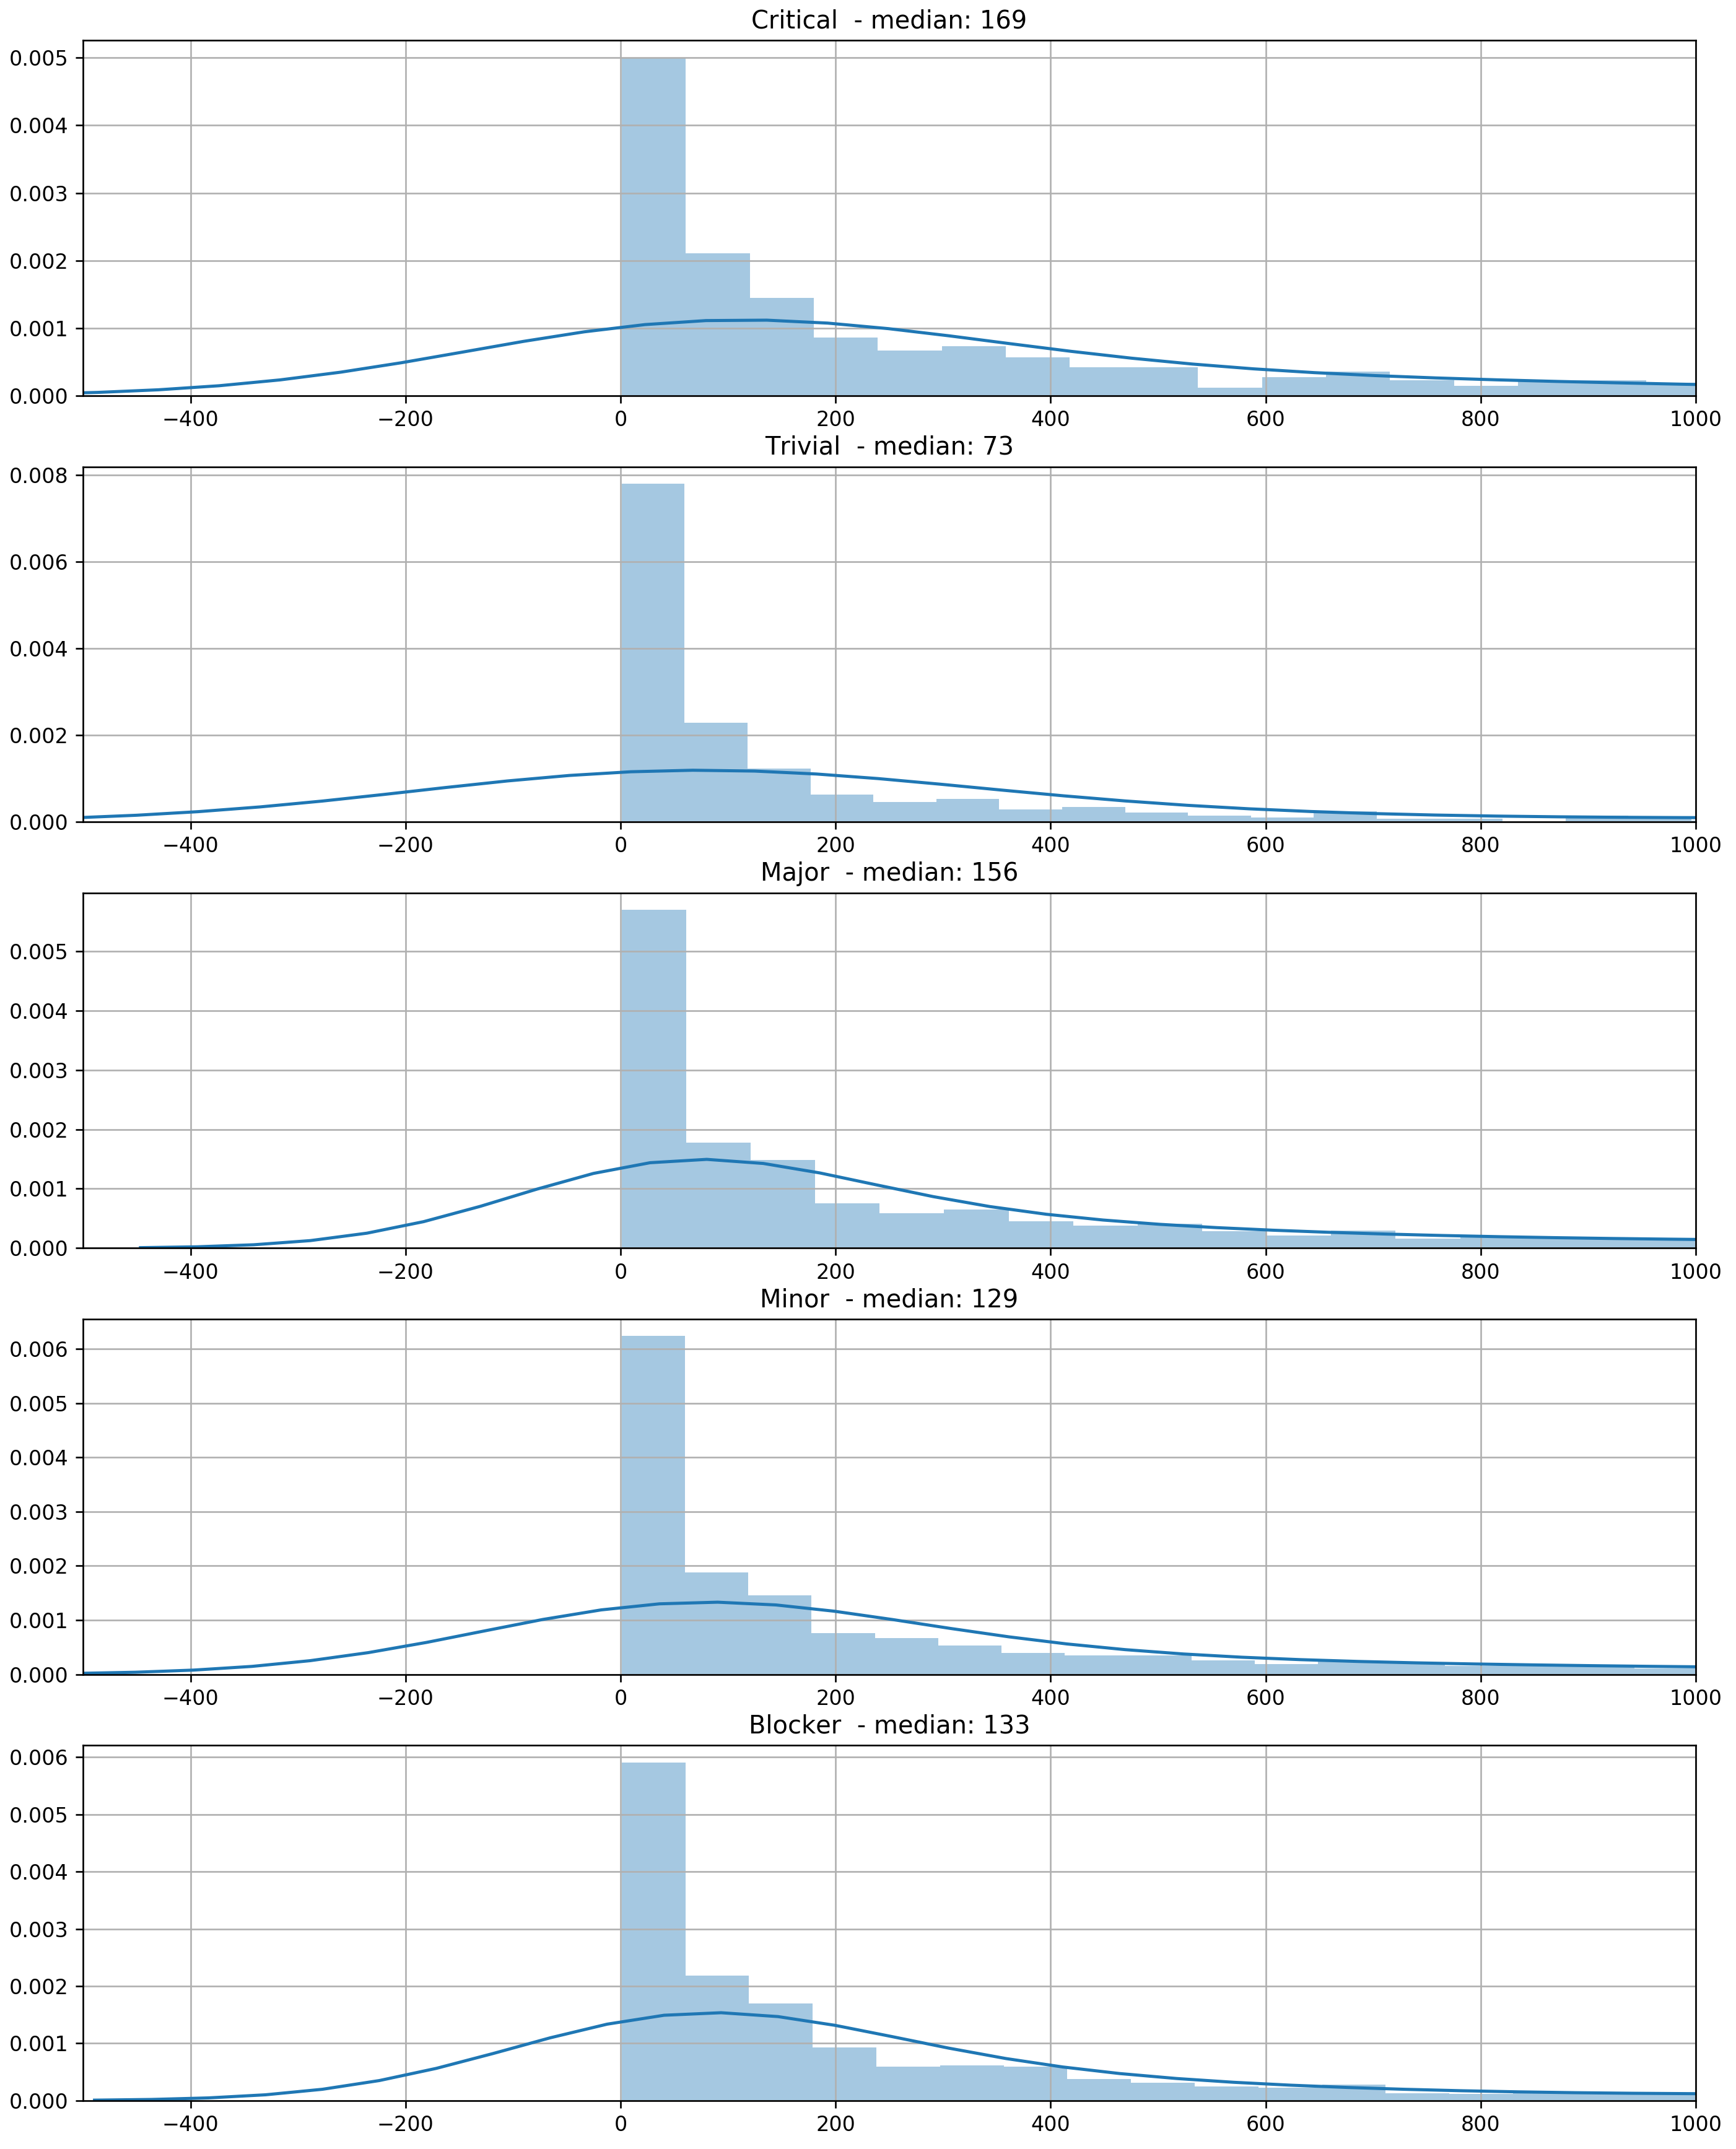
\includegraphics[width=\linewidth]{figure/duration_distr.png}
  \caption{Distribuzione durata per etichetta di priorità}
  \label{fig:duration_distr}
\end{figure}
Normalizzando il valore medio di ciascuna etichetta rispetto a tutte le altre è possibile ottenere il rapporto reciproco, questo valore verrà poi applicato per tradurre le etichette testuali. Utilizzando questo valore si ottiene una sorta di sforzo medio necessario alla risoluzione di problematiche di quella priorità. La distribuzione è stata calcolata su un dataset leggermente ristretto, sono state filtrate tutte le issue con un tempo di risoluzione inferiore ai 60 minuti (1h) o con un tempo maggiore di 6 mesi (4320h).
Con la nuova formulazione i valori di traduzione diventerebbero:
\begin{center}
  \captionof{table}{Valori numeri priorità con distribuzione} \label{tab:priority_distr}
  \begin{tabular}{ |c|c|c|c|c| }
     \hline
     \textbf{Critical} & \textbf{Major} & \textbf{Blocker} & \textbf{Minor} & \textbf{Trivial} \\
     \hline
     \hline
     26.0 & 24.0 & 20.0 & 20.0 & 11.0 \\
     \hline
  \end{tabular}
\end{center}
Ovviamente ogni progetto avrà valori differenti. La sostituzione delle etichette non ha richiesto particolari implementazioni ed è stata svolta a livello di script Python. L'utilizzo di questa modalità di traduzione ha portato ad un miglioramento nelle prestazioni del modello.\\
Questo parametro appena calcolato svolgerà la funzione di target, il valore quindi da predirre, rispetto ai file generati. Volendo valutare la predizione su differenti orizzonti temporali, nello specifico: 1, 2, 4, 6, 8, 10, 12, 16, 20, 30, 40 e 52 settimane. Per ogni settimana verrà calcolato la severity delle nuove issue aperte, moltiplicando il numero di issue per ogni categoria di priorità, per il valore definito dall'analisi, stesso calcolo viene fatto per le issue in chiusura, calcolando quindi la differenza tra questi due valori verrà definita la severity delle issue attive in quella settimana. Questo parametro diventerà il valore oggetto della predizione. Per generare i diversi lassi temporali verrà semplicemente applicato uno scambio di riga uguale al numero di settimane su cui sviluppare la predizione.\\
In concomitanza di questa informazione verrà aggiunta quella del conteggio di issue attive.


\paragraph{Trend matematici} una qualiasi previsione è fortemente dipendente dal comportamento del fenomeno nei momenti antecedenti alla valutazione. Esistono innumerevoli formulazioni matematiche per descrivere l'andamento di una curva. Nel nostro caso sono stati estratti alcuni parametri per informare la rete riguardo all'andamento tenuto. Chiaramente questi valori sono direttamente correlati al target ovvero il valore che intendiamo prevedere nel nostro sistema, la severity, e si riferisco ad essa:
\begin{itemize}
  \item \textit{exp\_avg}: media di tutti i valori precedenti a quel momento
  \item \textit{mov\_avg2}: media delle due settimane antecedenti a quella in esame
  \item \textit{mov\_avg4}: media delle quattro settimane antecedenti a quella in esame
  \item \textit{1before:} valore della settimana precedente
  \item \textit{2before:} valore di due settimane prima
  \item \textit{4before:} valore di quattro settimane prima
\end{itemize}
Il calcolo di questi valori è stato effettuato sfruttando le funzionalità contenute in Pandas, sfruttando principalmente i metodi: \textit{df.expanding()}, \textit{df.rolling()} e \textit{df.shift()}
Introduzione di questi parametri si è rivelata fondamentale nell'aiuto del modello, la relazione logica è facilmente comprensibile, la rimozione di questi parametri porta al crollo quasi totale del modello.


% #######################################
% #             Forecasting             #
% #######################################

\chapter{Previsione}
\label{chap:forecasting}
\section{Introduzione}
La previsione è il processo di effettuare predizione sul futuro basandosi su dati del passato e del prensente analizzando gli andamenti. La previsione è una delle funzionalità più desiderate tra gli algoritmi di apprendimento automatico, può facilmente migliorare qualsiasi processo, da quelli finanziari a quelli industriali. Ovviamente non è un obbiettivo semplice, effettuare ottime predizioni richiesta grande analisi, conoscenza e studio del fenomeno.\\
L'idea della previsione in questo ambito è quella di poter migliora e meglio allocare le risorse umane disponibili per lo sviluppo dei progetti. Assegnare troppe persone ad un task o troppi task ad una persona porterebbe ad una sicura riduzione dell'efficenza nello sviluppo.\\
Tutta questa fase di predizione fa riferimento al sotto progetto:
\begin{lstlisting}[language=Python, frame=single, basicstyle=\small]
  thesisProjectJN/ForecastAnalysis/
\end{lstlisting}
il file \textit{main.py} ha lo scopo di gestire l'avvio, nel file \textit{forecast.py} sono invece contenute le parti di codice relative agli specifici scenari.

\section{Modelli}
Nel capitolo \ref{chap:ml} sono stati trattati dal punto di vista tecnico matematico i modelli utilizzati nello svolgimento di questo progetto, ogungo di essi prensenta però parametri ed opzioni specifiche per il fenomeno che andranno a descrivere.\\
Il primo modello in esame è la foresta casuale, come valutato da \cite{santosh_se} \cite{Chen} \cite{super_unsuper} questo algoritmo si presta bene al fenomeno in questione. Il modello specifico è quello definito dalla libreria di SciKit, gli unici parametri personalizzati sono: il numero di alberi decisionali da implmentare, nel nostro caso, dopo alcuni tentativi di è deciso di scegliere 600 ed il numero di jobs, uno dei vantaggi degli algoritmi d'insieme è la possibilità di effettuare la fase di allenamento parallelizzandola, così facendo il tempo richiesto per tale fase si riduce enormemente.
\begin{lstlisting}[language=Python, frame=single, basicstyle=\small]
  from sklearn.ensemble import RandomForestRegressor
  ...
  ########### MODEL DEFINITIONS ###########
  predictor = 600
  n_jobs = 8
  model = RandomForestRegressor(n_estimators=predictor, 
                                  random_state=random, 
                                  verbose=verbose, 
                                  n_jobs=n_jobs)
\end{lstlisting}

Anche il modello ad aumento di gradiente è predefinito dalla libreria di SciKit:
\begin{lstlisting}[language=Python, frame=single, basicstyle=\small]
  from sklearn.ensemble import GradientBoostingRegressor
  ...
  ########### MODEL DEFINITIONS ###########
  predictor = 600
  model = GradientBoostingRegressor(n_estimators=predictor,
                                    random_state=random, 
                                    verbose=0)
\end{lstlisting}
il numero di stimatori è il medesimo di quello a foresta casuale. Nonostante sia un algoritmo d'insieme GBR non può applicare parallelizzazione, ogni step è sequenziale, la motivazione è meglio illustrata nel capitolo \ref{chap:ml}.\\
La rete neurale è molto più complessa, esistono molti modelli già definiti per l'analisi di fenomeni specifici, riconoscimento immagini, analisi sentimentale, ecc... Nell'esame della nostra problematica non è emersa letteratura riguardo l'applicazione di reti neurali, per questa motivazione è stata definita una rete abbastanza superificale, composta da 4 livelli sequenziali densi. Nello specifico è stata definita come segue:
\begin{lstlisting}[language=Python, frame=single, basicstyle=\small]
  def personal_model(shape):
    model = Sequential()
    model.add(Dense(shape, input_dim=shape, 
                    kernel_initializer='normal', 
                    activation='relu'))
    model.add(Dense(int(shape/2), activation='linear'))
    model.add(Dense(int(shape/4), activation='linear'))
    model.add(Dense(1, activation='linear'))
    model.compile(loss='mae', optimizer='adam', 
                    metrics=['msle'])

    return model
\end{lstlisting}
è stato valutando l'inserimento di diversi livelli, è stato per esempio valuto il dropout, ovvero un livello che casualmente spegnesse alcuni neuroni al fine di aumentare la randomicità del sistema ma, vista la contenuta quantità di dati, non ha portato alcun vantaggio al sistema.\\
Parlando di predizione temporale verrebbe chiaramente in mente di valutare l'opzione LSTM, nel nostro caso invece l'applicazione di tale struttura non porta vantaggi. L'obbiettivo infatti non è quello di dare una previsione per tempistiche indefinite effettuando quindi una previsione e applicando la successiva sul valore di uscita della precedente, ma la nostra previsione è puntuale, definito un istante $t_0$ andremo ad efettuare la nostra previsione a $t_0 + \textrm{weekly\_horizon}$, la previsione successiva avrà l'aggiornamento della situazione e non dovrà basarsi sui dati precedentemente predetti ma lo fara sui dati attuali di un preciso momento. Per questo motivo appena illustrato l'utilizzo di LSTM si è rivelato inconcludente e con pessimi risultati, il sistema in esame infatti ottime ottimi risultati quando la finestra di previsione varia.


\section{Metodologia}
L'applicazione di modelli statistici di apprendimento automatico si articola in due fasi principali: allenamento e predizione.\\
La prima fase di formazione prevede che il modello venga allenato utilizzando grandi quantità di dati in modo da renderlo indipendente e preparato per la successiva fase nella quale verrà impegnato per la predizione.\\
La procedura di allenamento non è assolutamente banale, il modello non è in grado di capire a priori quali siano i punti cardine del nostro fenomeno, per questo motivo è importante offrirgli dei dati puliti, controllati e valutati. Una cattiva impronta nella fasi iniziali potrebbe facilemente portare a pessime prestazioni nella fase di predizione.\\
Sono state scelte tre differenti modalità di allenamento, prendendo esempio da \cite{Chen} e \cite{super_unsuper}: singolo scenario, cross-version e cross-project. È importante considerare come le previsioni effettuate con i modelli a foresta e ad aumento di gradiente mantengono risultati quasi identici tra le differenti esecuzioni, è infatti sufficiente definire un valore casuale per l'avvio della fase di allenamento. Nel caso invece della rete neurale non è possibile congelare l'inilizzializzazione dei pesi del sistema, per questo motivo sono stati riportati i migliori valori attenuti da ripetute esecuzioni dello stesso ambiente.

\paragraph{Singolo scenario} è l'applicazione rispetto, al nostro fenomeno, della classica procedura di training-predict ovvero che un singolo file o blocco di dati viene dato alla rete per effettuare sia la fase di allenamento, sia la fase di test. Solitamente i dati vengono divisi in due blocchi, appunto allenamento e test, con percentuali 70\% e 30\%, o 75\% e 25\%. La divisione può avvenire in diversi modi, sia casuale quindi scambio i dati a livello temporale, sia a blocco mantenendo quindi l'ordine originale. Essendovi un reale vincolo logico tra questi dati non è stato possibile applicare la prima modalità, rompere il flusso naturale del fenomeno avrebbe chiaramente forviato l'apprendimento.\\
In questo specifico caso la divisione applicata è stata 75\% e 25\%. Il procedimento di divisione è stato affidato a SciKit, una volta letto il file in ingresso e separata la colonna del valore da predirre è stato sufficiente applicare quanto segue:
% \vspace{10em}
\begin{lstlisting}[language=Python, frame=single, basicstyle=\small]
  
  labels = np.array(features['n'])
  mean = np.mean(labels)
  features = features.drop('n', axis=1) 
  
  feature_list = list(features.columns) 
  features = np.array(features)
  
  train_features, test_features, train_labels, test_labels = \
      train_test_split(features, labels, 
                        test_size=test_size, 
                        random_state=random, 
                        shuffle=False)
\end{lstlisting}
Un volta effettuata la divisione nei due set è possibile procedere con la definizione del modello di apprendimento automatico da utilizzare, con il modello pronto è possibile procedere alla fase di allenamento vera e propria, questa fase viene gestita tutta dalla libreria di Keras. Questa fase può avere una durata anche notevole, nel nostro caso la quantità di informazioni non è esagerata quindi il processo di formazione dura qualche minuto. Una volta terminata questa fase il modello è allenato e pronto ad essere utilizzato per la previsione. In questo caso la predizione verrà fatta sulla porzione di dati non utilizzata nella fase di allenamento, il 30\%. Verranno presi in esame due casi: il file con la versione 2 di hadoop ed il file con la versione 2 di hbase.\\
L'applicazione dei tre modelli ha portato a questi risultati lungo le le diverse settimane:
\begin{center}
  \captionof{table}{Esecuzione singolo scenario: hadoop} \label{tab:single_scen_hadoop}
  \begin{tabular}{ |c|c|c|c|c|c|c|c|c|c|c| }
     \hline
     \textbf{Model} & \textbf{Metric} & \textbf{1w} & \textbf{2w} & \textbf{4w} & \textbf{8w} & \textbf{12w} & \textbf{16w} & \textbf{20w} & \textbf{30w}  & \textbf{52w} \\
     \hline
     \hline
     RF & R2 & 0.798 & 0.603 & 0.319 & - & - & - & - & - & -\\
     \hline
     RF & P & 55.0\% & 41.2\% & 23.4\% & - & - & - & - & - & -\\
     \hline
     \hline
     GB & R2 & 0.805 & 0.515 & 0.08 & - & - & - & - & - & -\\
     \hline
     GB & P & 52.4\% & 33.4\% & 0.0\% & - & - & - & - & - & -\\
     \hline
     \hline
     NN & R2 & 0.980 & 0.96 & 0.916 & 0.660 & 0.111 & - & - & - & -\\
     \hline
     NN & P & 87.4\% & 79.1\% & 69.0\% & 32.9\% & 0.0\% & - & - & - & -\\
     \hline
  \end{tabular}
\end{center}
Il grafico in figura \ref{fig:single_scenario_error} visualizza la tabella precedente.
\begin{figure}[!ht]
  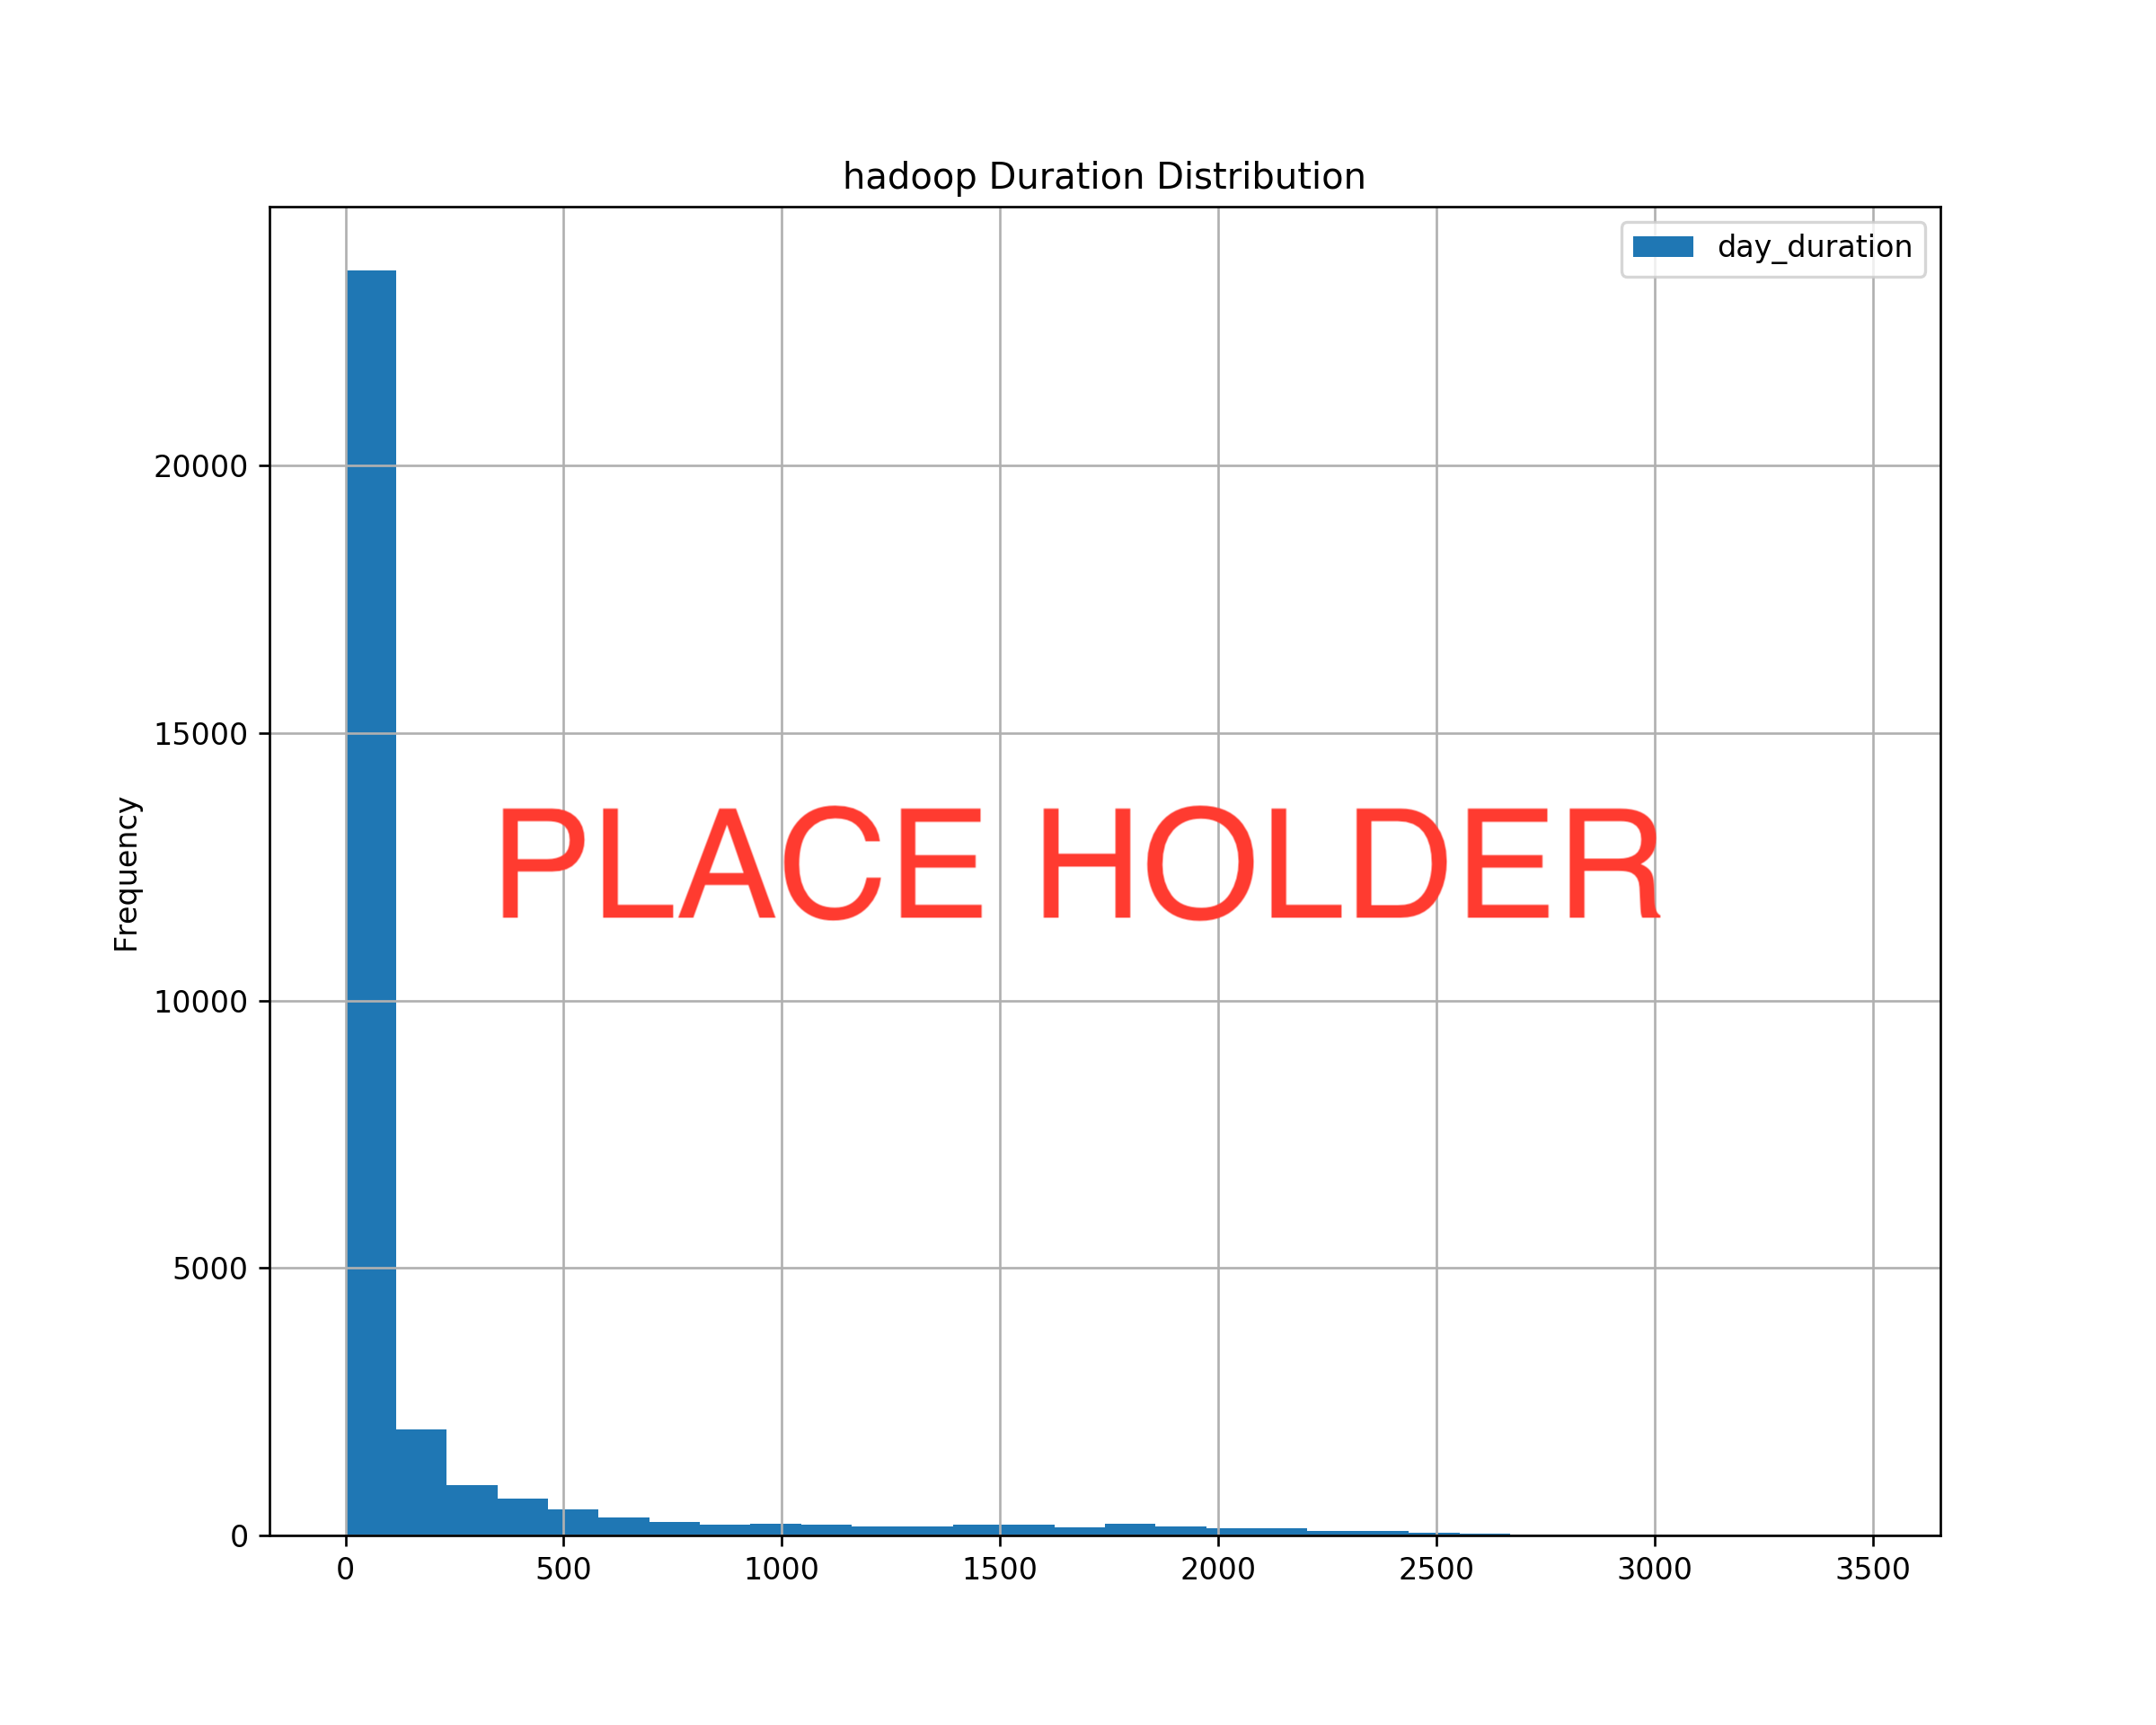
\includegraphics[width=\linewidth]{figure/place_holder.png}
  \caption{Andamento errori singolo scenario}
  \label{fig:single_scenario_error}
\end{figure}
\begin{figure}[!ht]
  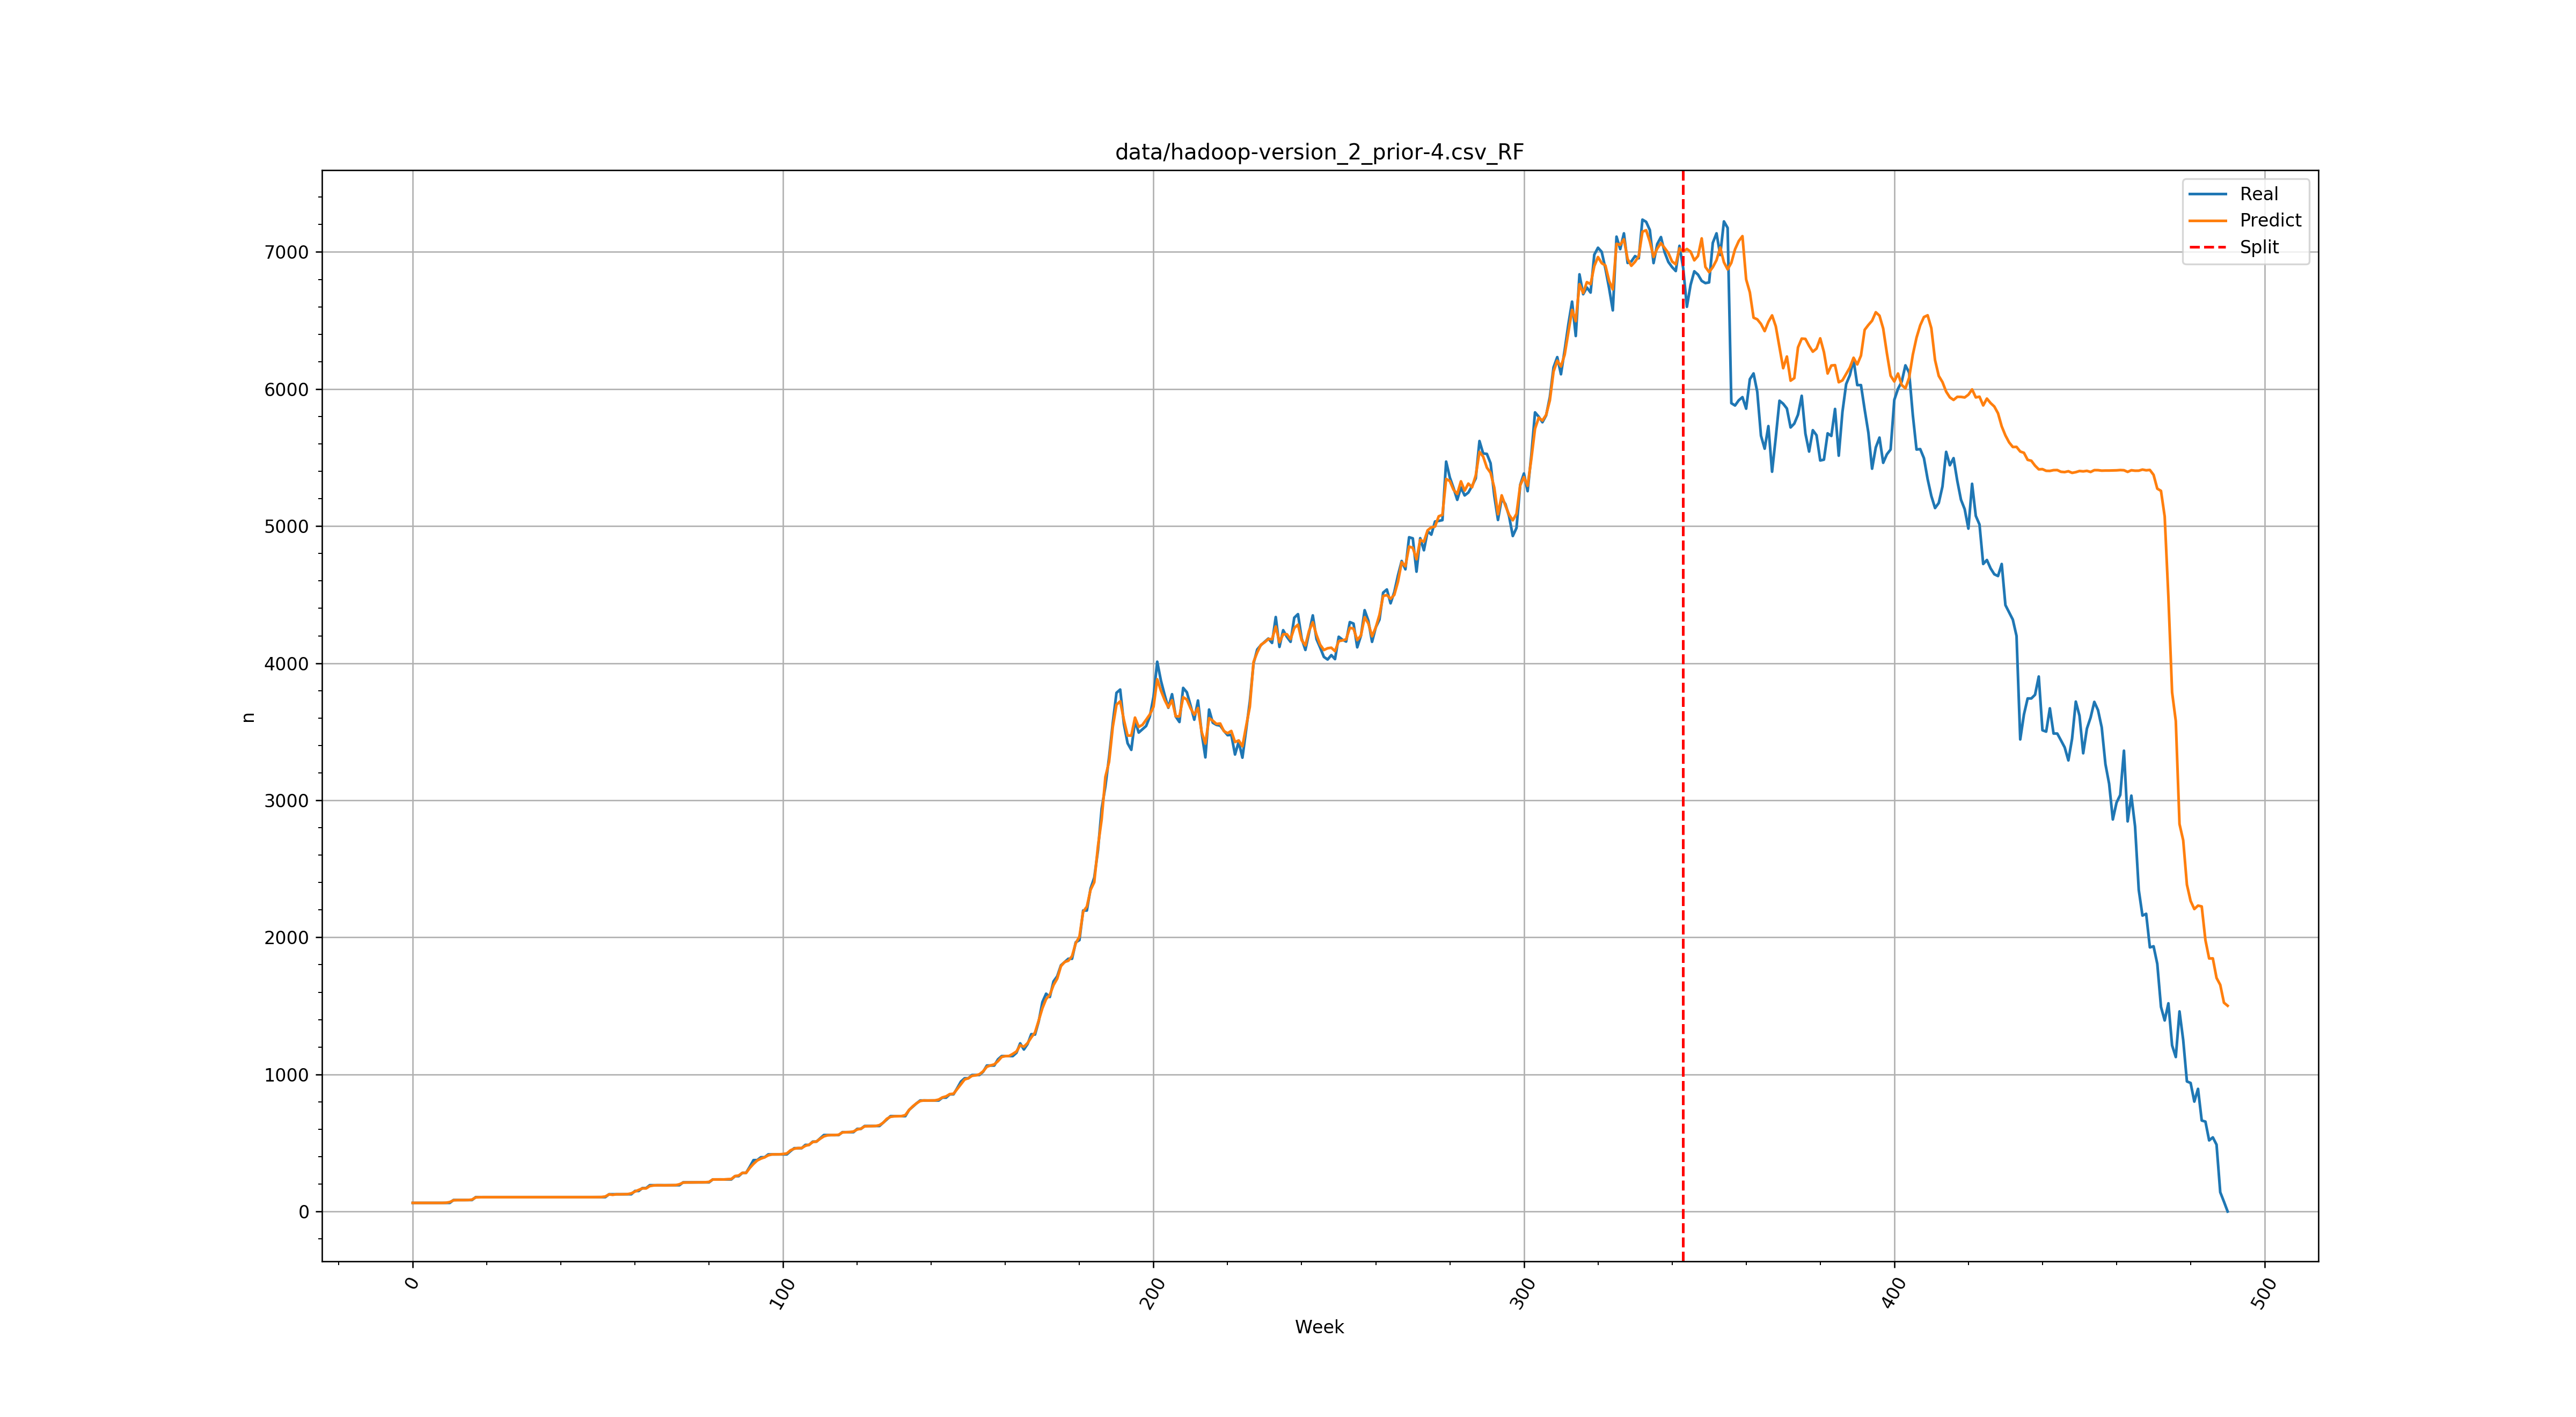
\includegraphics[width=\linewidth]{figure/hadoop_rf_4w.png}
  \caption{hadoop RF a 4 settimane}
  \label{fig:hadoop_rf_4w}
\end{figure}

L'applicazione di questa metodologia non porta a grandissimi risultati, per nessun tipo di modello in esame. La motivazione di ciò è facilmente ricorducibile alla modalità di applicazione della metodologia stessa. Come si può notare dal grafico in figura \ref{fig:hadoop_rf_4w}, l'allenamento viene effettuato solamente sulla parte crescente della curva, di conseguenza nessuno dei modelli viene allenato a prevedere una discesa del fenomeno.\\
I risultati non sono differenti se applicati un differente progetto, infatti:
\begin{center}
  \captionof{table}{Esecuzione singolo scenario: hbase} \label{tab:single_scen_hbase}
  \begin{tabular}{ |c|c|c|c|c|c|c|c|c|c|c| }
    \hline
    \textbf{Model} & \textbf{Metric} & \textbf{1w} & \textbf{2w} & \textbf{4w} & \textbf{8w} & \textbf{12w} & \textbf{16w} & \textbf{20w} & \textbf{30w}  & \textbf{52w} \\
    \hline
    \hline
    RF & R2 & 0.701 & 0.554 & 0.027 & - & - & - & - & - & -\\
    \hline
    RF & P & 52.5\% & 48.0\% & 28.9\% & - & - & - & - & - & -\\
    \hline
    \hline
    GB & R2 & 0.540 & 0.035 & - & - & - & - & - & - & -\\
    \hline
    GB & P & 39.8\% & 20.0\% & - & - & - & - & - & - & -\\
    \hline
    \hline
    NN & R2 & 0.925 & 0.811 & 0.597 & - & - & - & - & - & -\\
    \hline
    NN & P & 76.4\% & 65.7\% & 50.9\% & - & - & - & - & - & -\\
    \hline
  \end{tabular}
\end{center}
Il grafico riporta un previsione della rete neurale applicata ad hbase con previsione di 4 settimane.
\begin{figure}[!ht]
  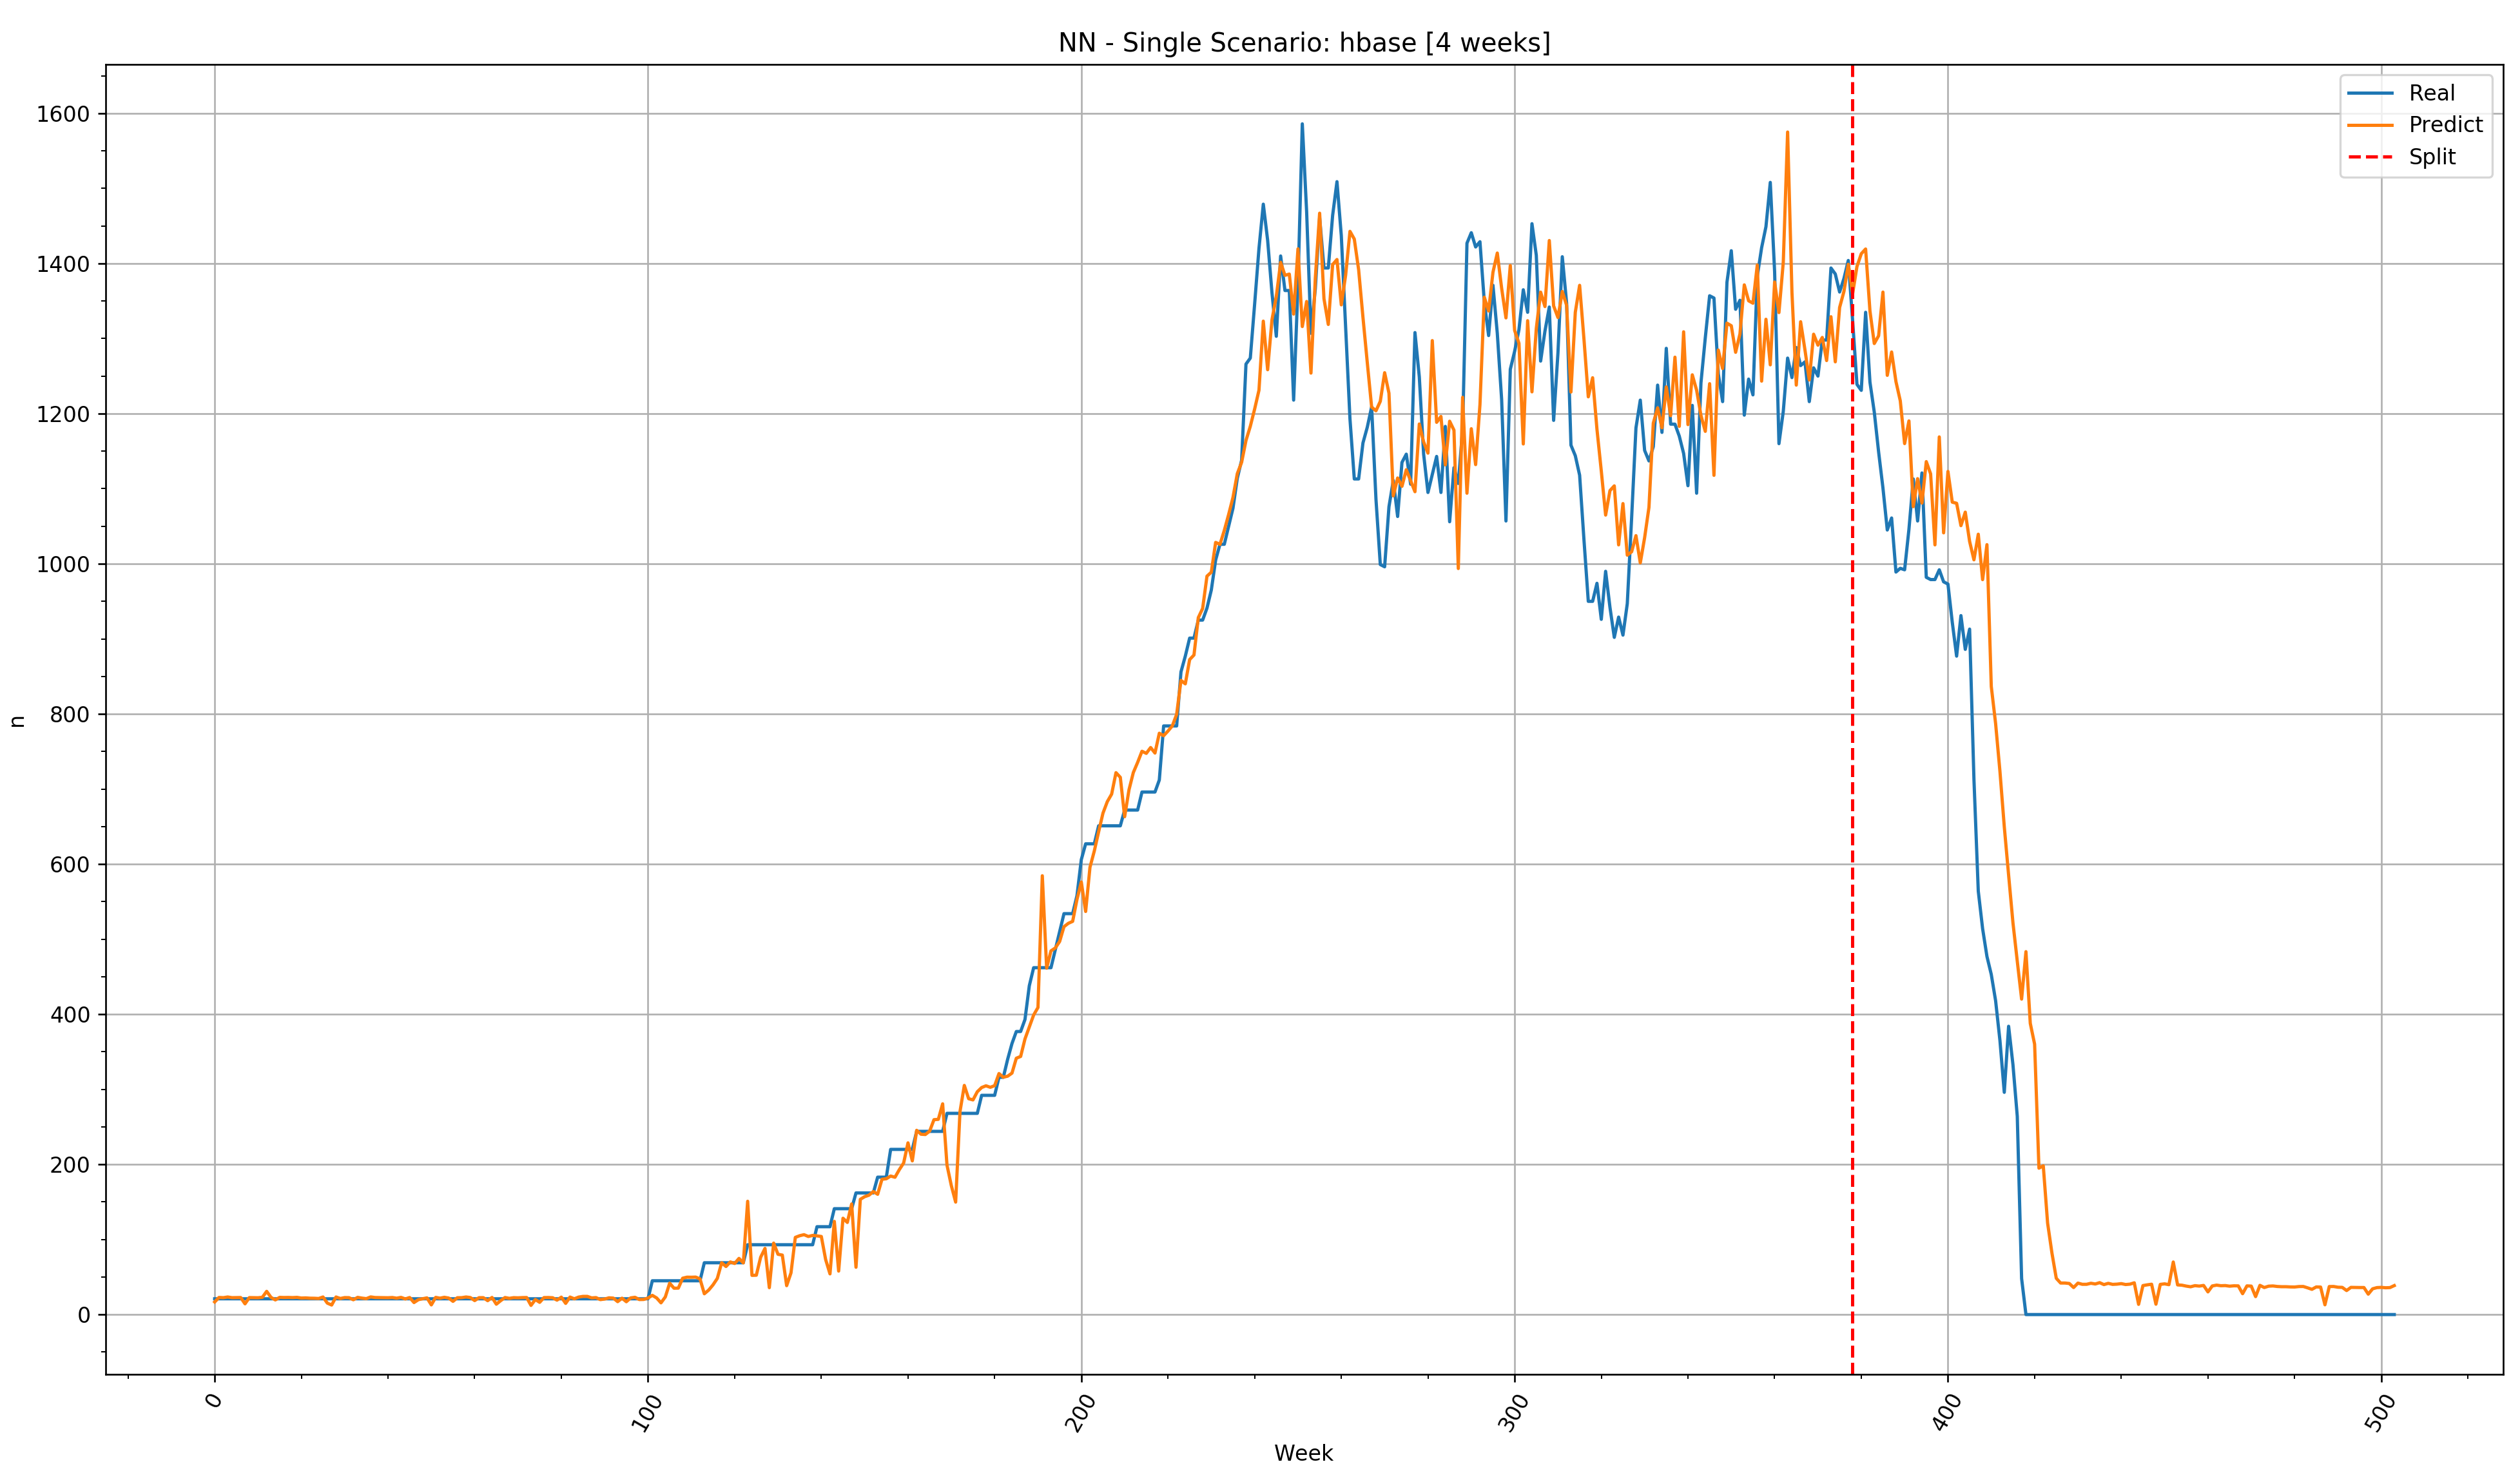
\includegraphics[width=\linewidth]{figure/hbase_nn_4w.png}
  \caption{hbase NN a 4 settimane}
  \label{fig:hbase_nn_4w}
\end{figure}
Alcuni dati sono stati omessi, sostituiti con il trattino, per la mancanza di rilevanza, l'errore generato era esageramente elevato e conseguentemente non significativo.
Utilizzando l'esempio di hbase, il quale presenta una serie di discese importanti, è possibile notare come, aggiungendo delle fasi descrescenti nei dati utilizzati durante la fase di allenamento, il sistema riesce a migliorare enormemente la sua capacità di previsione nella fase di chiusura, addattandosi quindi meglio ai dati da seguire con un conseguente miglioramento dei risultati.

\paragraph{Cross-version} L'applicazione della strategia precedente presenta un errore logico intrinseco, il modello difficilmente veniva allenato su fasi discendenti di severity, di conseguenza non poteva apprenderne il comportamento, motivo della pessima qualità dei risultati. L'idea della modalità cross-version mira proprio a risolvere questa problematica. La possibilità di allenare la rete su diverse versioni di sviluppo dello stesso progetto permette di imparare sia il comportamente generico della comunità ad esso legata, sia le diverse fasi di avvio e conclusione di un rilascio.\\
Ogni progetto in esame ha una differente storia di sviluppo, di conseguenza un numero diverso di issue e settimane di sviluppo, per questo motivo si è deciso di sviluppare un sistema flessibile che permettesse all'utilizzatore di effettuare il training su un numero non specificato di versioni differenti. Oltre il differente numero di rilasci, un ipotetico utilizzatore, potrebbe voler trascurare una versione nel training di questo modello; solitamente le prime versioni di un progetto, nel caso di quelli open source, sono molto scarne, poco seguite e non molto strutturate, via via che il progetto guadagna interesse la comunità si espande, portando così ad una crescita di tutte le componenti ad esso legate. Una visualizzazione di questa situazioni si ha in figura \ref{fig:cassandra_vers}, dove la prima versione è notevolmente meno strutturata delle successive.
\begin{figure}[!ht]
  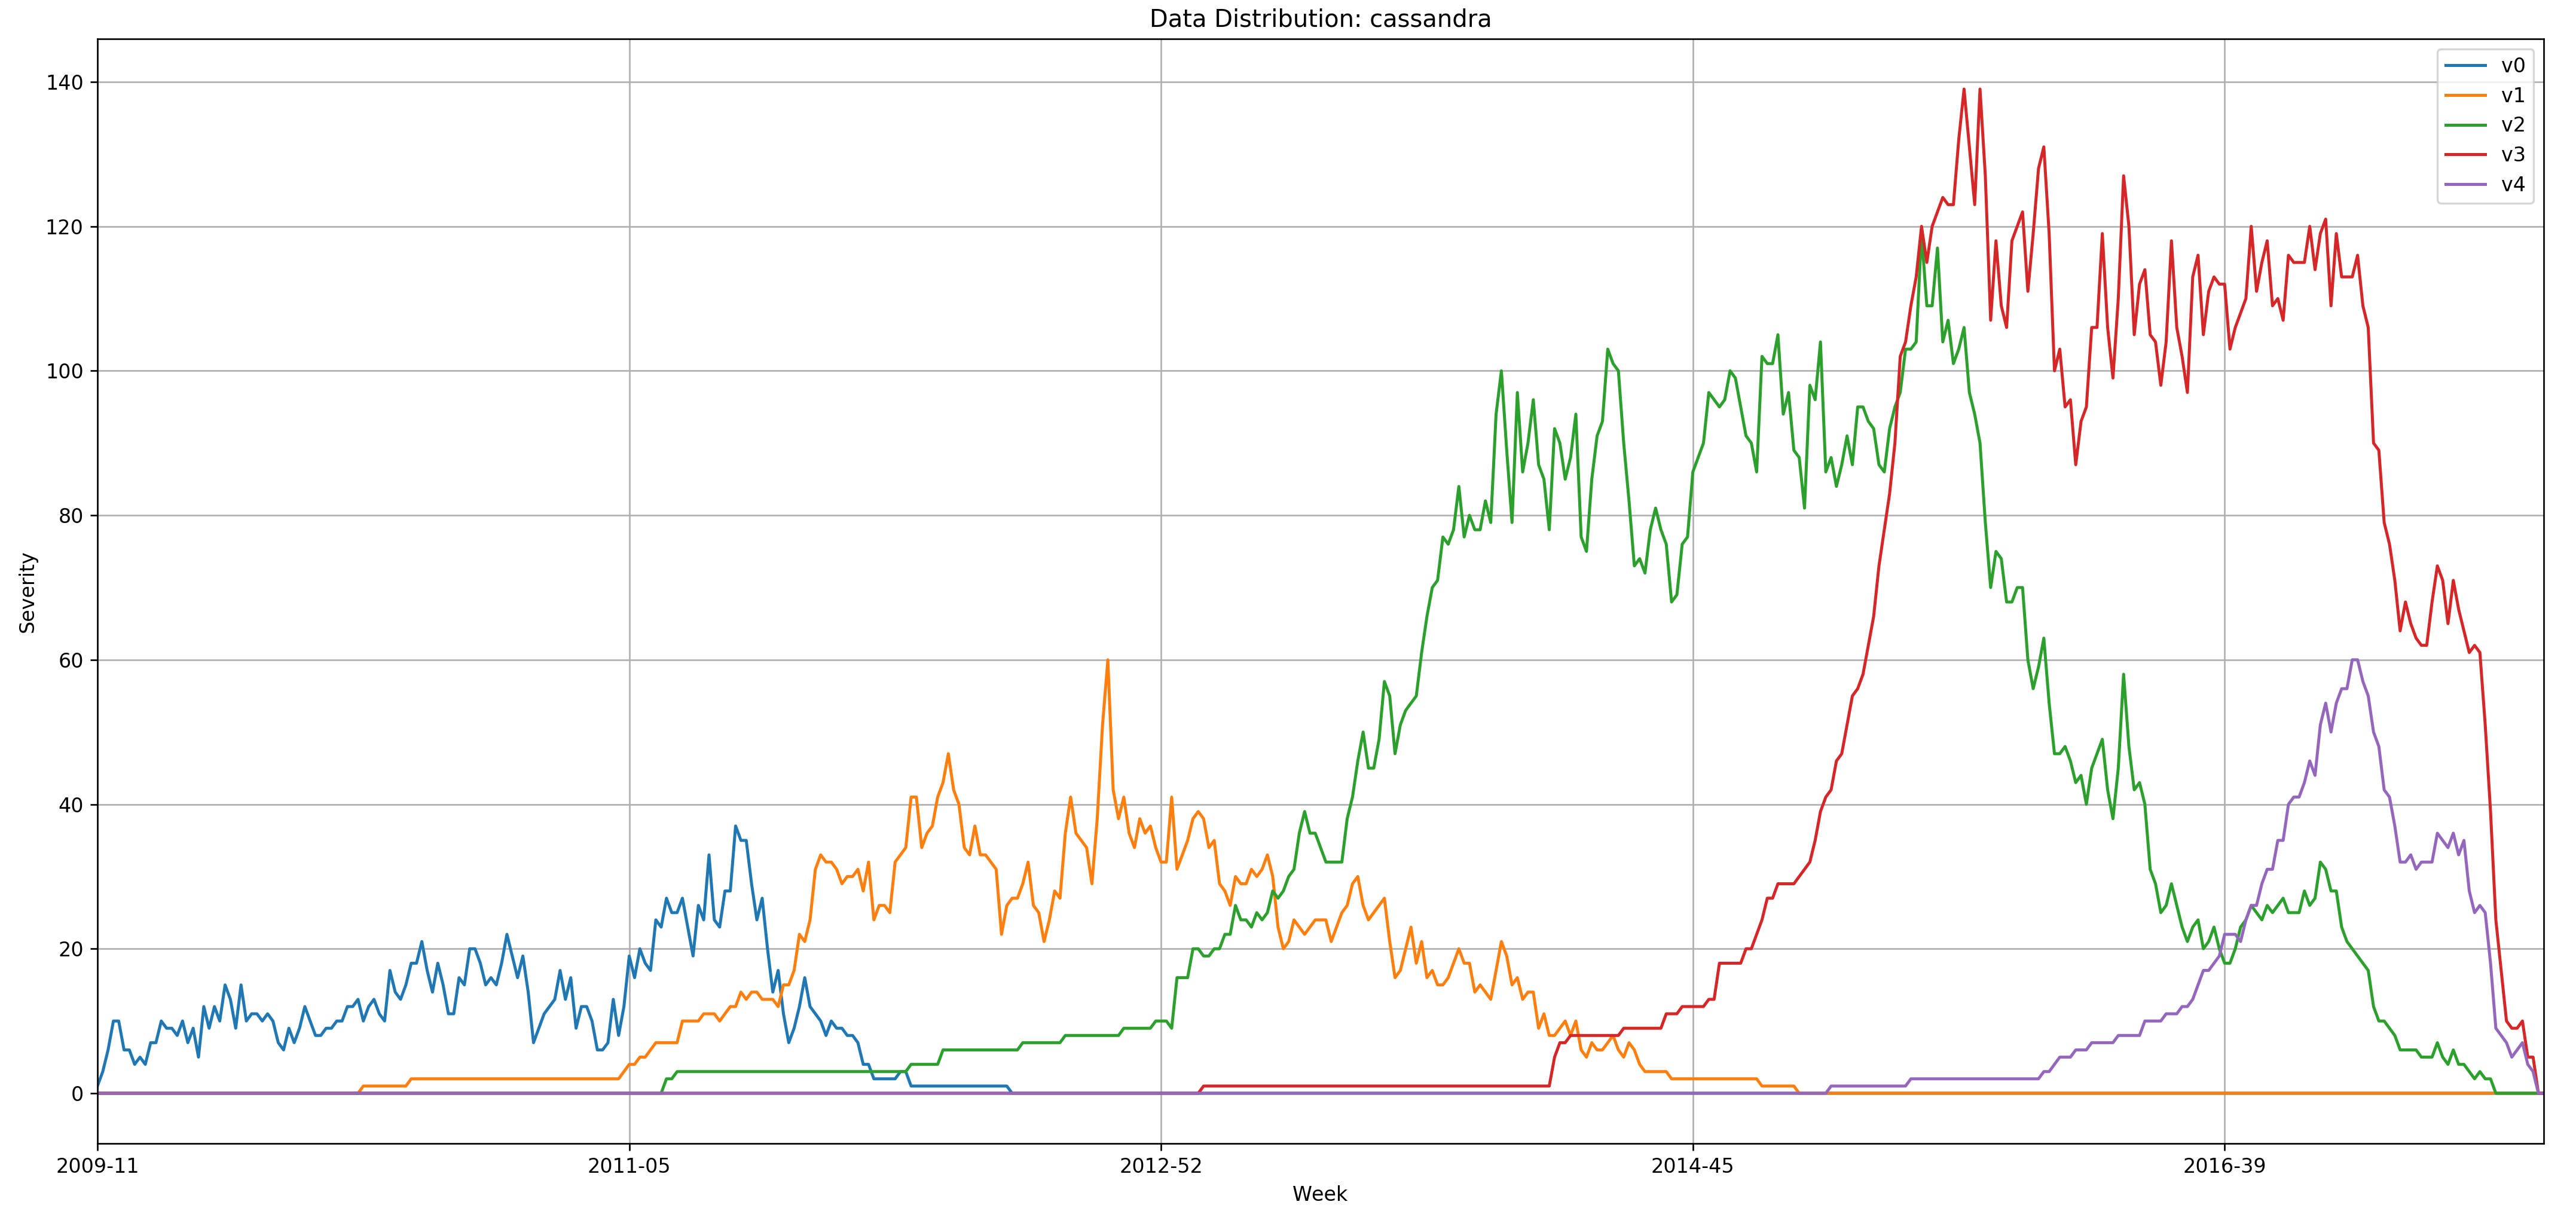
\includegraphics[width=\linewidth]{figure/cassandra_vers.png}
  \caption{Distribuzione issue per versione in Cassandra}
  \label{fig:cassandra_vers}
\end{figure}
Applicando quindi la fase di formazione, per esempio, alle prime tre versioni permetterà al modello di conoscere bene l'andamento del fenomeno per la quarta versione.\\
La successiva tabella visualizza i punteggi, lungo le differenti finestre temporali, rispetto ai 3 differenti modelli, applicando il training sulle versione v0, v1, v2 e prevedendo la versione v3 del progetto Cassandra:
\begin{center}
  \captionof{table}{Esecuzione cross-version: Cassandra} \label{tab:cross_version_cassandra}
  \begin{tabular}{ |c|c|c|c|c|c|c|c|c|c|c| }
    \hline
    \textbf{Model} & \textbf{Metric} & \textbf{1w} & \textbf{2w} & \textbf{4w} & \textbf{8w} & \textbf{12w} & \textbf{16w} & \textbf{20w} & \textbf{30w}  & \textbf{52w} \\
    \hline
    \hline
    RF & R2 & 0.964 & 0.945 & 0.846 & 0.743 & - & - & - & - & -\\
    \hline
    RF & P & 69.7\% & 73.7\% & 66.8\% & 34.3\% & - & - & - & - & -\\
    \hline
    \hline
    GB & R2 & 0.961 & 0.924 & 0.842 & 0.716 & - & - & - & - & -\\
    \hline
    GB & P & 46.8\% & 83.4\% & 46.2\% & 9.0\% & - & - & - & - & -\\
    \hline
    \hline
    NN & R2 & 0.988 & 0.975 & 0.961 & 0.591 & 0.875 & 0.620 & 0.423 & 0.648 & -\\
    \hline
    NN & P & 88.8\% & 77.6\% & 74.6\% & 33.7\% & 59.0\% & 48.1\% & 21.5\% & 24.9\% & -\\
    \hline
  \end{tabular}
\end{center}
Per mantenere un filo comune alle tre modalità anche qui valuteremo la metodologia sul caso hadoop. Essendo il progetto ancora più grosso ed effettuando l'allenamento sulle versioni v0, v1 e v2, predicendo la v3 i risultati sono i seguenti:
\begin{center}
  \captionof{table}{Esecuzione cross-version: hadoop} \label{tab:cross_version_hadoop}
  \resizebox{\textwidth}{!}{
  \begin{tabular}{ |c|c|c|c|c|c|c|c|c|c|c| }
    \hline
    \textbf{Model} & \textbf{Metric} & \textbf{1w} & \textbf{2w} & \textbf{4w} & \textbf{8w} & \textbf{12w} & \textbf{16w} & \textbf{20w} & \textbf{30w}  & \textbf{52w} \\
    \hline
    \hline
    RF & R2 & 0.995 & 0.992 & 0.984 & 0.957 & 0.918 & 0.858 & 0.805 & 0.607 & -\\
    \hline
    RF & P & 87.9\% & 86.9\% & 82.5\% & 79.5\% & 73.4\% & 65.4\% & 61.2\% & 46.9\% & -\\
    \hline
    \hline
    GB & R2 & 0.995 & 0.992 & 0.984 & 0.951 & 0.926 & 0.873 & 0.791 & 0.497 & -\\
    \hline
    GB & P & 88.2\% & 88.3\% & 80.8\% & 77.5\% & 74.8\% & 68.8\% & 60.1\% & 42.7\% & -\\
    \hline
    \hline
    NN & R2 & 0.981 & 0.993 & 0.988 & 0.961 & 0.955 & 0.905 & 0.846 & 0.771 & 0.096\\
    \hline
    NN & P & 86.4\% & 88.9\% & 89.2\% & 80.4\% & 72.9\% & 60.3\% & 51.3\% & 47.1\% & 20.9\%\\
    \hline
  \end{tabular}
  }
\end{center}
I vantaggi dell'applicazione di questa strategia di allenamento sono visibili, nella precedente strategia le predizioni si presentavano insignificanti anche dopo poche settimane. Permettere al modello di valutare anche le fasi discendenti dello sviluppo consente un notevole miglioramento della qualità delle previsioni, entro le 4 settimane i risultati superano quasi sempre il valore di 85\%. I risultati rimangono inoltre abbastanza elevati lungo tutte le settimane e la caduta di precisione è nettamente inferiore rispetto a quella del modello a scenario singolo. Nello spefico si può notare come la rete neurale abbia risultati migliori rispetto agli altri due algortimi testati.

\paragraph{Cross-project} l'ultima metodologia valutata è quella tra progetti. Potrebbe sembrare insensato mettere a confronto diversi progetti e la loro storia di sviluppo, ogni comunità ha le proprie modalità di rapporto, sviluppo e tanto altro, difficilmente queste differenti situazioni potrebbero mantenere andamenti similari. In realtà, come si dimostrerà successivamente, questa soluzione sarà quella con i migliori risultati, la possbilità di visualizzare situazioni differenti lo rende più flessibile ed adattabile ai vari contesti, inoltre, la sorgente dei dati, SEOSS33, aveva proprio lo scopo di riuscire a generalizzare il più possibile diversi progetti open, in modo da rendere confrontabili i risultati.\\
L'utilizzo di questa metologia è molto particolare e la sua applicazione nella realtà diventa molto complessa, l'ottenimento di questi ottimi risultati è direttamente correlato alla antecedente valutazione dei dati scelti per la fase di allenamento, si è infatti deciso di selezionare andamenti in modo oculato, che presentassero differenti casistiche, rapide salite e discese, valori proporzionati e altri fattori. In molti casi il modello cross-project potrebbe portare a risultati peggiori rispetto a quello cross-version.\\
La prima esecuzione riguarda il progetto di hadoop, ambiente comune a tutte e tre le metodologie. I dati utilizzati per questa esecuzione sono:
\begin{itemize}
  \item hadoop v2
  \item cassandra v2
  \item hbase v1
\end{itemize}
mentre hadoop v3 sarà la versione sulla quale verranno effettuate le previsioni. In questo caso si è deciso di mantenere un blocco di dati dello stesso progetto e due di progetti differenti, la motivazione risiede in hadoop stesso, essendo un progetto con numeri decisamente più grandi degli altri, senza poter visualizzare situazioni con numeri simili, i modelli allenati non erano in grado di avvicinarsi ai dati della versione 3. L'esecuzione ha portato i risultati visualizzati in tabella \ref{tab:cross_project_hadoop}.
\begin{center}
  \captionof{table}{Esecuzione cross-project: hadoop} \label{tab:cross_project_hadoop}
  \resizebox{\textwidth}{!}{
  \begin{tabular}{ |c|c|c|c|c|c|c|c|c|c|c| }
    \hline
    \textbf{Model} & \textbf{Metric} & \textbf{1w} & \textbf{2w} & \textbf{4w} & \textbf{8w} & \textbf{12w} & \textbf{16w} & \textbf{20w} & \textbf{30w}  & \textbf{52w} \\
    \hline
    \hline
    RF & R2 & 0. & 0. & 0. & 0. & 0. & 0. & 0. & 0. & -\\
    \hline
    RF & P & \% & \% & \% & \% & \% & \% & \% & \% & -\\
    \hline
    \hline
    GB & R2 & 0. & 0. & 0. & 0. & 0. & 0. & 0. & 0. & -\\
    \hline
    GB & P & \% & \% & \% & \% & \% & \% & \% & \% & -\\
    \hline
    \hline
    NN & R2 & 0. & 0. & 0. & 0. & 0. & 0. & 0. & 0. & 0.\\
    \hline
    NN & P & \% & \% & \% & \% & \% & \% & \% & \% & \%\\
    \hline
  \end{tabular}
  }
\end{center}
L'andamento è abbastanza stabile lungo tutte le esecuzioni, i risultati leggermente migliori, ma molto simili a quelli con la metodologia cross-version, questo perchè effettivamente l'unica differenza in gioco è il dato di ingresso. In figura \ref{fig:hadoop_cp_nn_4w} viene riportata una delle previsioni effettuate.
\begin{figure}[!ht]
  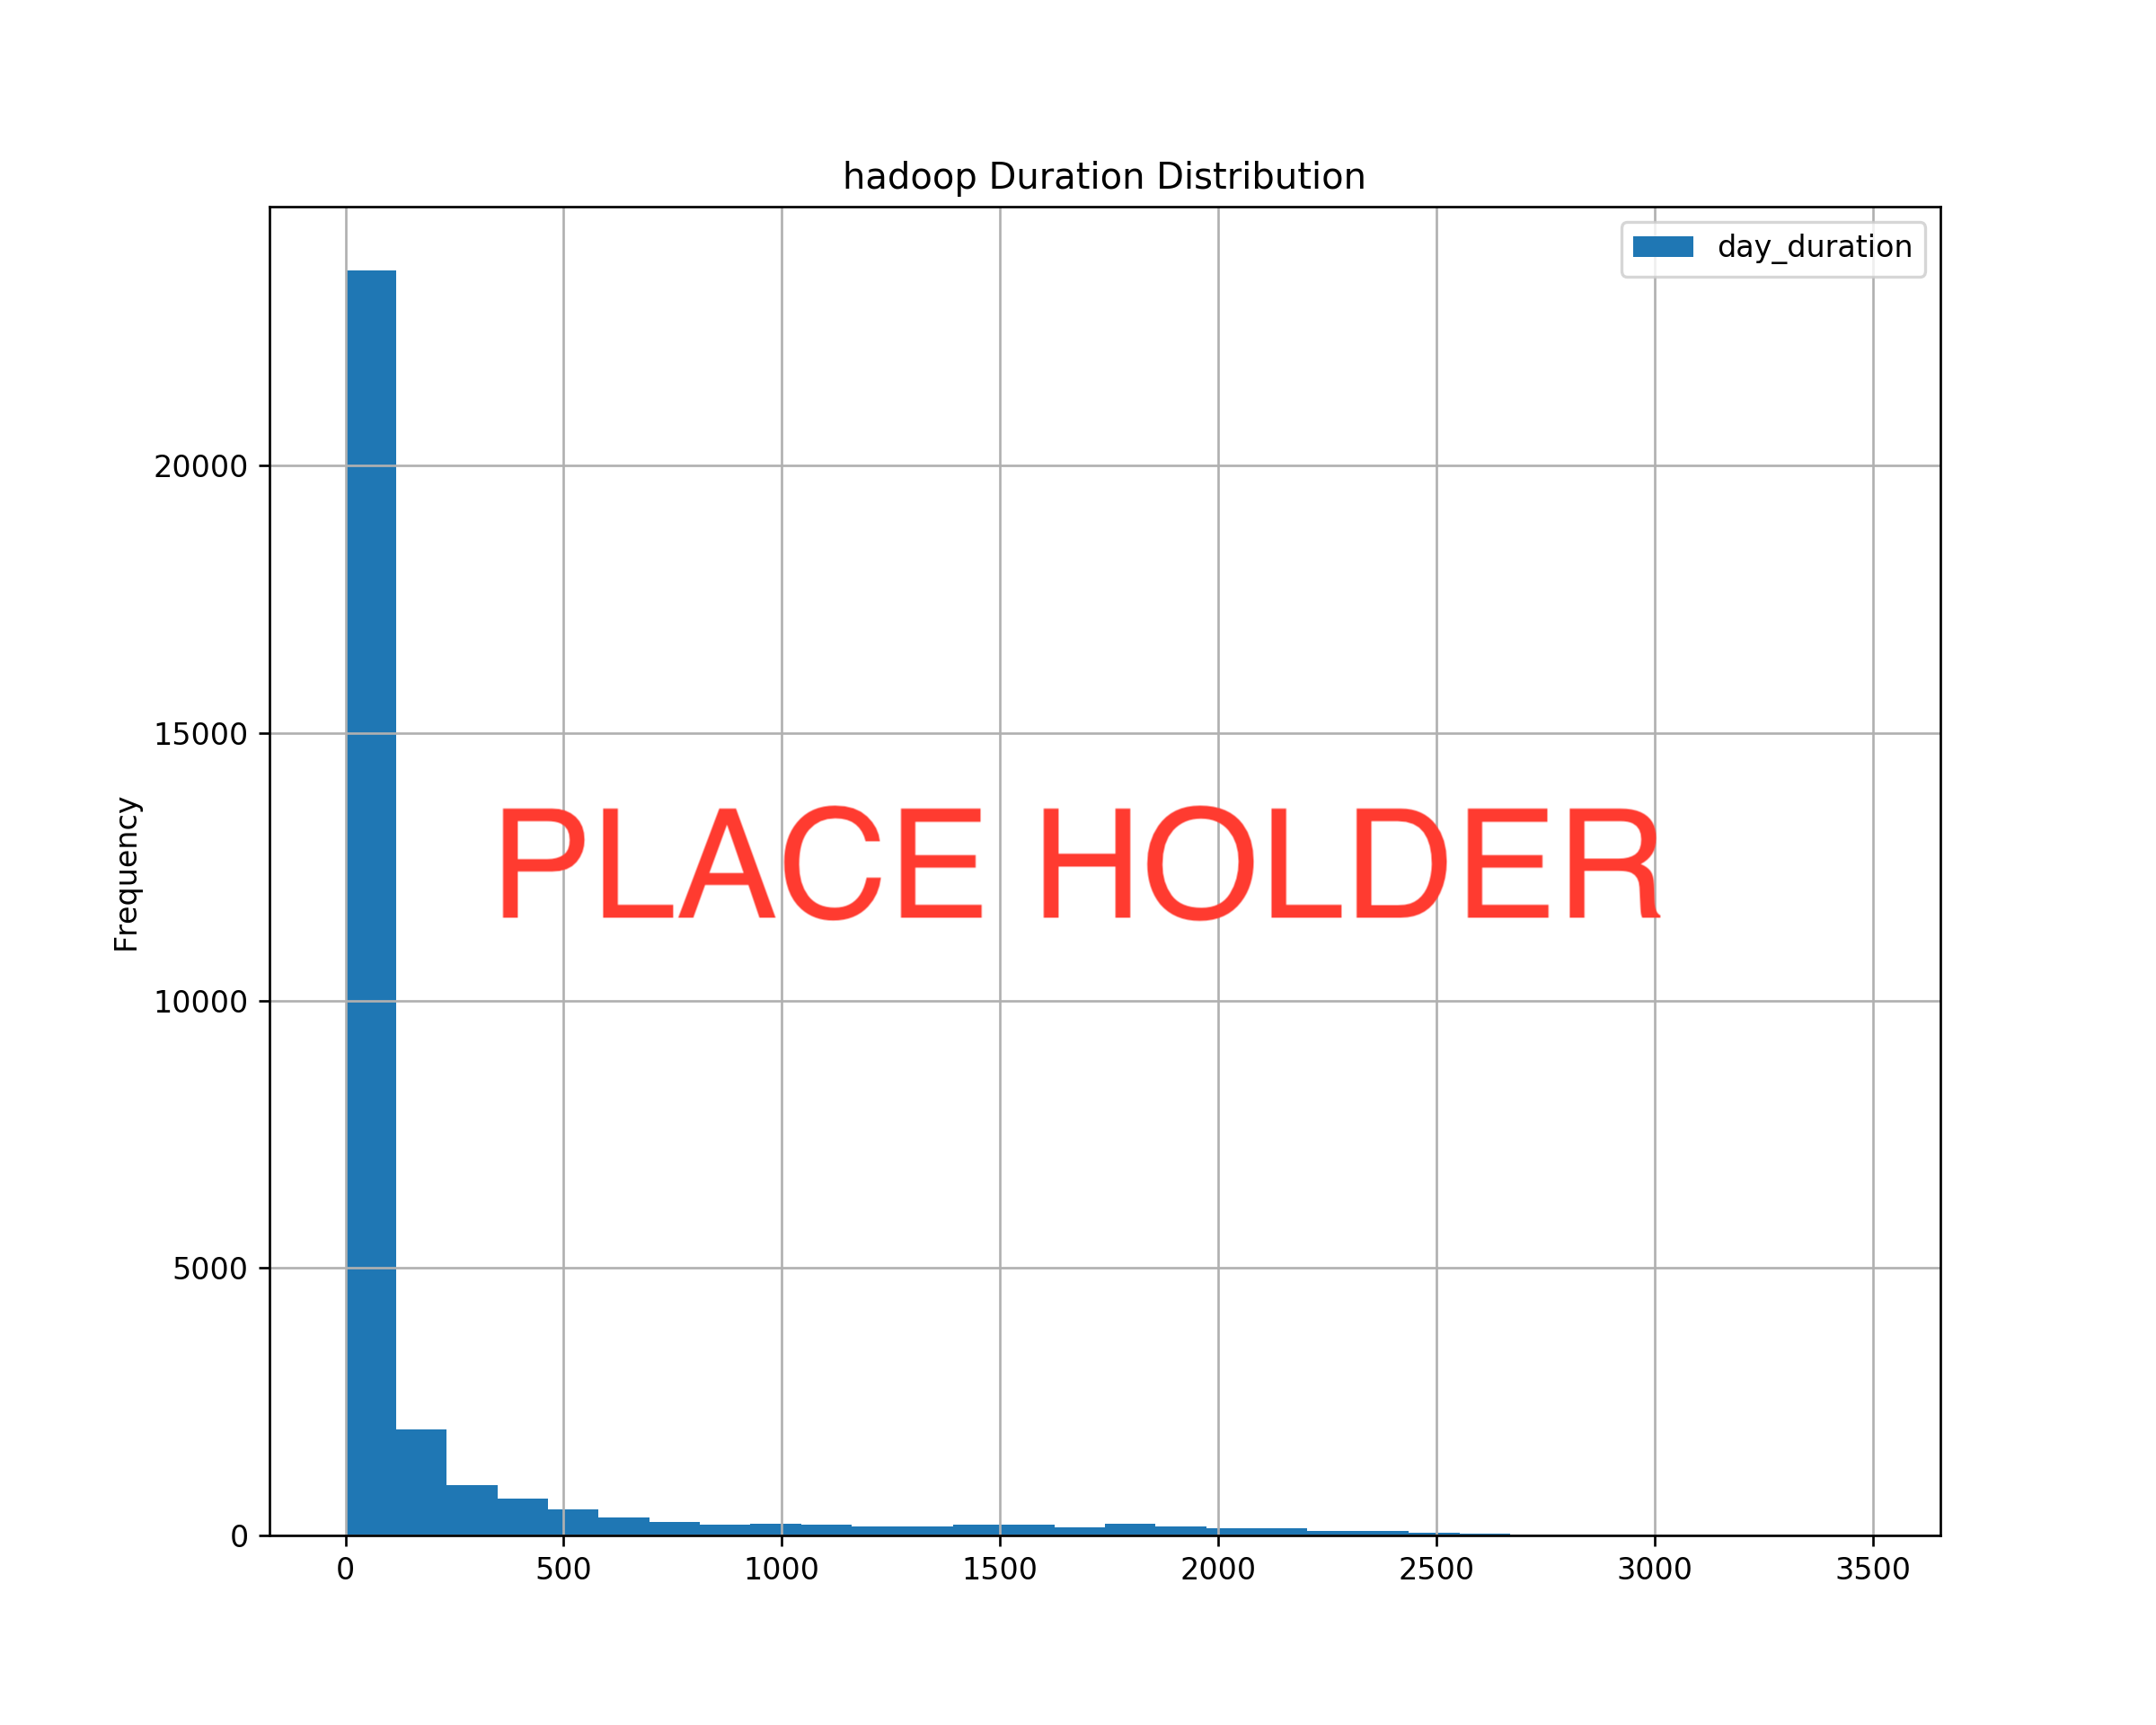
\includegraphics[width=\linewidth]{figure/place_holder.png}
  \caption{Previsione a 4 settimane cross-project per hadoop v3}
  \label{fig:hadoop_cp_nn_4w}
\end{figure}

La seconda esecuzione, quella con i risultati migliori di tutti è applicata sul progetto cassandra, i dati utilizzati per la fase di allenamento del modello sono:
\begin{itemize}
  \item hadoop v0
  \item hbase v1
  \item hive v2
\end{itemize}
i migliori risultati delle varie esecuzioni sono i riportati in tabella \ref{tab:cross_project_hadoop}.
\begin{center}
  \captionof{table}{Esecuzione cross-project: hadoop} \label{tab:cross_project_hadoop}
  \resizebox{\textwidth}{!}{
  \begin{tabular}{ |c|c|c|c|c|c|c|c|c|c|c| }
    \hline
    \textbf{Model} & \textbf{Metric} & \textbf{1w} & \textbf{2w} & \textbf{4w} & \textbf{8w} & \textbf{12w} & \textbf{16w} & \textbf{20w} & \textbf{30w}  & \textbf{52w} \\
    \hline
    \hline
    RF & R2 & 0. & 0. & 0. & 0. & 0. & 0. & 0. & 0. & -\\
    \hline
    RF & P & \% & \% & \% & \% & \% & \% & \% & \% & -\\
    \hline
    \hline
    GB & R2 & 0. & 0. & 0. & 0. & 0. & 0. & 0. & 0. & -\\
    \hline
    GB & P & \% & \% & \% & \% & \% & \% & \% & \% & -\\
    \hline
    \hline
    NN & R2 & 0. & 0. & 0. & 0. & 0. & 0. & 0. & 0. & 0.\\
    \hline
    NN & P & \% & \% & \% & \% & \% & \% & \% & \% & \%\\
    \hline
  \end{tabular}
  }
\end{center}
L'immagine \ref{fig:cassandra_cp_nn_4w} visualizza la previsione effettuata su questa versione.
\begin{figure}[!ht]
  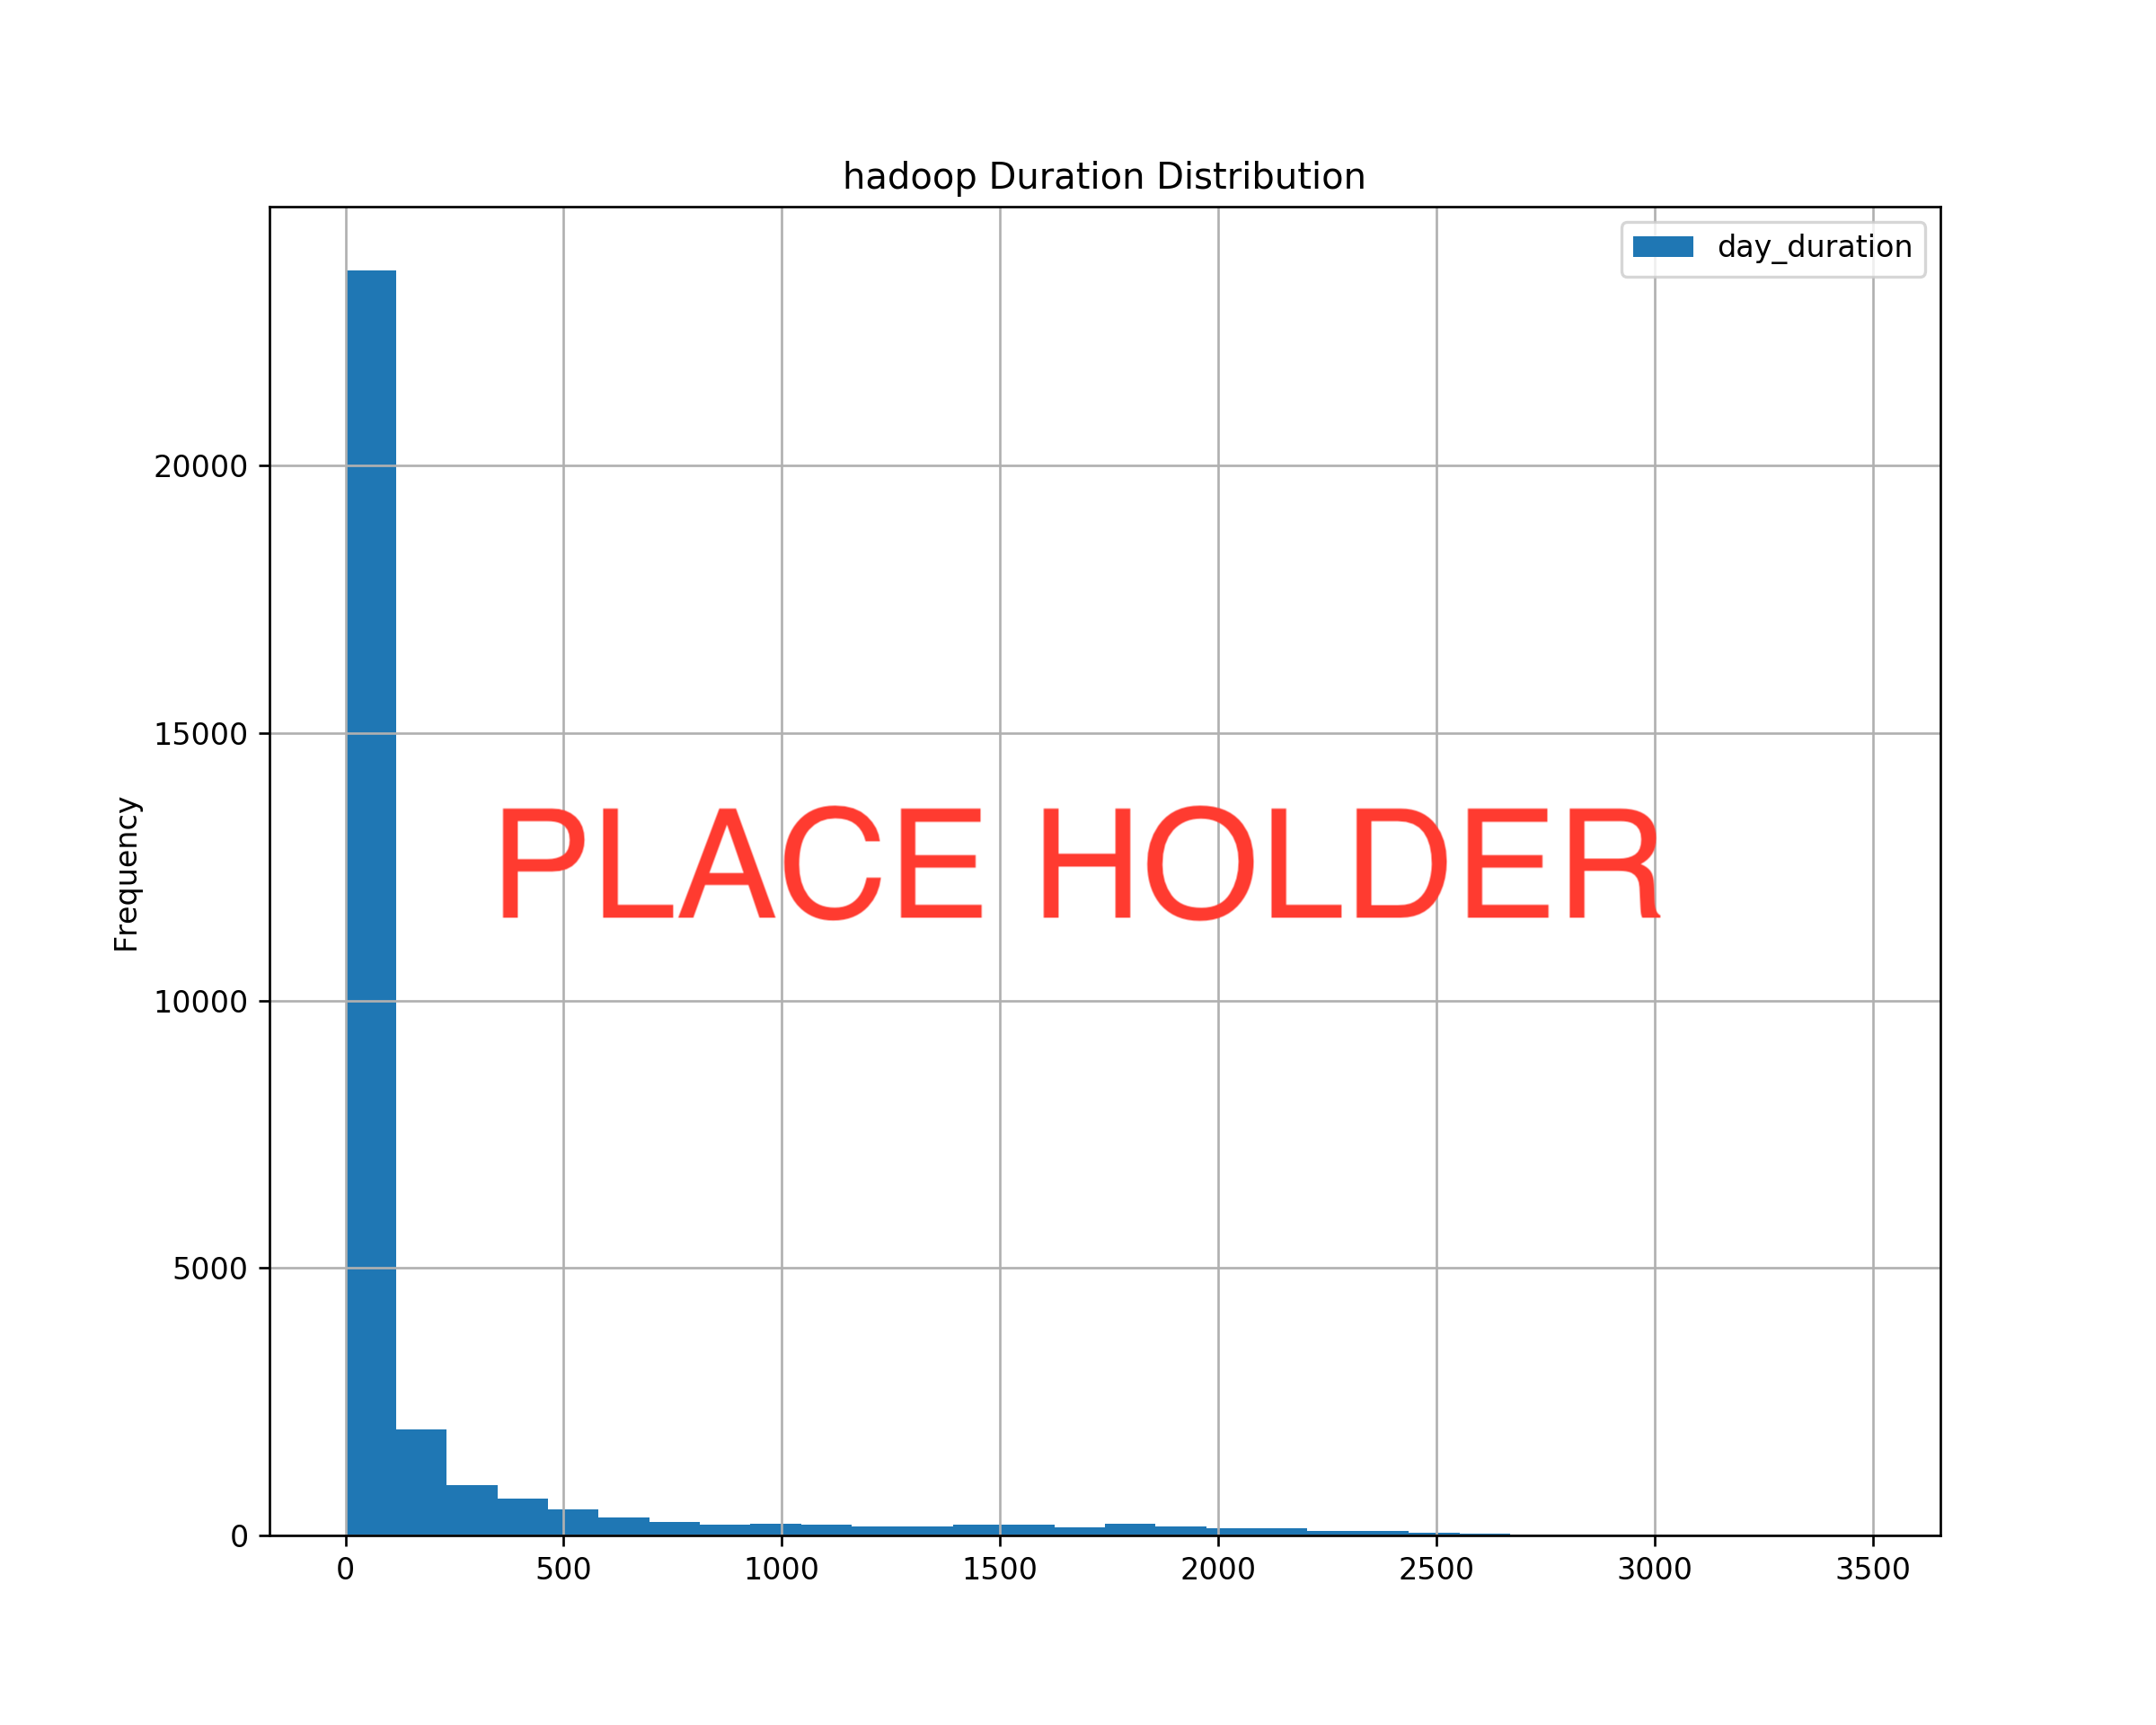
\includegraphics[width=\linewidth]{figure/place_holder.png}
  \caption{Previsione a 4 settimane cross-project per cassandra v2}
  \label{fig:cassandra_cp_nn_4w}
\end{figure}


% #######################################
% #             Conclusion              #
% #######################################

\chapter{Conclusioni}
Il progetto trattato in questo elaborato prendere in considerazione la previsione di un fenomeno per poter meglio allocare le risorse necessarie allo sviluppo dello stesso, la metodologia utilizzata si basa su algoritmi di intelligenza artificiale e calcolo statistico.\\


% #######################################
% #            BIBLIOGRAPHY             #
% #######################################
\bibliography{biblio}
\bibliographystyle{QUICKtran}


\end{document}
